% =====================================================================
%  Exponential ergodicity and the space-time Gibbs states of
%  one-dimensional probabilistic cellular automata
%  Seth Douglas and Nidhal Mghirbi
%  Version 1.2.0, November 2026
%
%  Build: python -B build.py (three pdflatex passes; see README.txt)
%  The numbers in Section 11.3 are produced by verification/code/majority_certificates.py;
%  its recorded output is verification/code/majority_certificates_output.txt.
%  The checks of Sections 11.6 and 13 added in version 1.2.0 are in verification/v1.2/.
% =====================================================================
\documentclass[11pt]{article}
\usepackage[a4paper,margin=27mm,top=28mm,bottom=30mm]{geometry}
\usepackage[T1]{fontenc}
\usepackage[utf8]{inputenc}
\usepackage{mathpazo}
\usepackage[scaled=0.92]{helvet}
\usepackage{microtype}
\usepackage{amsmath,amssymb,amsthm,mathtools}
\usepackage{booktabs,array,tabularx}
\usepackage{enumitem}
\usepackage{tikz}
\usetikzlibrary{calc,patterns,decorations.pathreplacing}
\usepackage[colorlinks=true,linkcolor=black!70!blue,citecolor=black!60!blue,urlcolor=black!60!blue]{hyperref}
\usepackage[capitalise,noabbrev]{cleveref}
\usepackage{caption}
\captionsetup{font=small,labelfont=bf,width=0.92\textwidth}

\setlist{itemsep=2pt,topsep=3pt}
\linespread{1.04}

\theoremstyle{plain}
\newtheorem{theorem}{Theorem}[section]
\newtheorem{proposition}[theorem]{Proposition}
\newtheorem{lemma}[theorem]{Lemma}
\newtheorem{corollary}[theorem]{Corollary}
\theoremstyle{definition}
\newtheorem{definition}[theorem]{Definition}
\newtheorem{example}[theorem]{Example}
\newtheorem{problem}[theorem]{Open problem}
\theoremstyle{remark}
\newtheorem{remark}[theorem]{Remark}
\newtheorem*{mainA}{Theorem A}
\newtheorem*{mainB}{Theorem B}
\newtheorem*{mainC}{Theorem C}
\newtheorem*{mainD}{Theorem D}
\newtheorem*{mainE}{Theorem E}
\newtheorem*{mainF}{Theorem F}
\newtheorem*{mainG}{Theorem G}

\newcommand{\A}{\mathcal{A}}
\newcommand{\Z}{\mathbb{Z}}
\newcommand{\N}{\mathbb{N}}
\newcommand{\R}{\mathbb{R}}
\newcommand{\Q}{\mathbb{Q}}
\newcommand{\E}{\mathbb{E}}
\newcommand{\Prob}{\mathbb{P}}
\newcommand{\dtv}{d_{\mathrm{TV}}}
\newcommand{\dH}{d_{\mathrm{H}}}
\newcommand{\Lam}{\Lambda}
\newcommand{\eps}{\varepsilon}
\newcommand{\ba}{\bar{\mu}}
\newcommand{\cl}{\operatorname{cl}}
\newcommand{\dist}{\operatorname{dist}}
\newcommand{\Cov}{\operatorname{Cov}}
\newcommand{\Var}{\operatorname{Var}}
\newcommand{\osc}{\operatorname{osc}}
\newcommand{\sgn}{\operatorname{sgn}}
\newcommand{\tsup}{\operatorname{supp}}
\newcommand{\Ue}{\mathrm{U}}
\newcommand{\hatD}{\widehat{\Delta}}
\newcommand{\Sd}{S_{\mathrm{d}}}
\newcommand{\Tf}{\mathcal{T}}
% Depth-7 row of Table 2; the numbers are from verification/code/majority_certificates_output.txt.
\newcommand{\MAJSEVEN}{7 & $97/200$ & $0.9930$ & $\MAJSEVENA$ & $\MAJSEVENB$\\}
\newcommand{\MAJSEVENA}{0.2091}
\newcommand{\MAJSEVENB}{0.8333}

\hypersetup{pdftitle={Exponential ergodicity and the space-time Gibbs states of one-dimensional probabilistic cellular automata},pdfauthor={Seth Douglas and Nidhal Mghirbi}}
\title{\vspace{-1.2cm}\LARGE Exponential ergodicity and the space--time Gibbs states\\ of one-dimensional probabilistic cellular automata}
\author{Seth Douglas \and Nidhal Mghirbi}
\date{\small Version 1.2.0, November 2026}

\begin{document}
\maketitle

\begin{abstract}
\noindent
A positive-rate probabilistic cellular automaton (PCA) defines a Gibbs specification in one more dimension, its space--time interaction, in which the future is a boundary like the past and the sides. For finite-alphabet, finite-radius, strictly positive PCA on~$\Z$ we prove that uniform exponential ergodicity of the dynamics is equivalent to exponential weak spatial mixing of this specification in arbitrary finite volumes of~$\Z^2$ under arbitrary exterior conditions, so that the specification has exactly one DLR state, the stationary trajectory law, with exponentially decaying correlations. This answers in one dimension, under exponential ergodicity, the question of Lebowitz, Maes and Speer whether every Gibbs measure of the space--time interaction is a trajectory law of the PCA, previously known for periodic measures. The forward proof removes the far future boundary from B\'erard's coupling from the past at an entropy cost that only one-dimensional geometry absorbs. In every dimension, cutting the cluster of coupling failures at a late level, where its accumulated size dominates its width, removes the future boundary whenever the dynamics has a coalescing local flow satisfying the quantitative small-badness hypothesis of the prefix-cap theorem. In particular, if some basic i.i.d.\ random-map representation coalesces exponentially for all inputs at once, the specification has exactly one DLR state and exponential weak mixing in arbitrary volumes, and for attractive binary PCA in every dimension uniform exponential ergodicity is equivalent to exponential weak mixing. In every dimension and with no rate, the relative-entropy defect of any Gibbs measure from the dynamics is a surface term; hence for an ergodic PCA the stationary trajectory is the only uniformly recurrent Gibbs measure, the translation action on the Gibbs simplex is uniquely ergodic, and all-DLR uniqueness holds exactly when every Gibbs measure is uniformly recurrent. Finite certificates for the hypothesis are exactly computable; for the noisy majority rule they give a unique space--time Gibbs state down to noise $0.485$, including noise one half, and Marsan, Sablik and T\"orm\"a's fixed radius-one automaton has one space--time Gibbs state at small noise (granting structural estimates from their low-noise proof) and at large noise, and several in between. Finally, as an explicit witness of a classical phenomenon, the synchronous heat-bath dynamics of the anisotropic Ising model at critical couplings is a positive PCA on $\Z^2$ with a rational table that is uniformly ergodic but not exponentially ergodic: granting two classical exact formulas for the Ising model, the largest distance between the laws of one site at time $t$ from two initial rows is at least $\frac14(t+1)^{-1/8}$.
\end{abstract}
\begin{center}\small AI systems assisted with this work. The authors take responsibility for its claims; see ``How this work was done.'' This preprint has not been peer reviewed.\end{center}
\begin{center}\small Programs and finite checks: \url{https://github.com/Apsiape/exponential-ergodicity-space-time-gibbs}.\end{center}

\tableofcontents

% =====================================================================
\section{Introduction}
% =====================================================================

\subsection{A dynamics is an equilibrium system in one more dimension}
\label{sec:intro}

A probabilistic cellular automaton on $\Z^d$ updates every site of a row independently, each site reading a finite neighbourhood of the preceding row through one fixed transition table $p(a\mid u)$. Run it forever and record every row: the result is a random configuration on $\Z^d\times\Z$. Multiply the transition probabilities of the sites in a finite space--time volume: the product is a Boltzmann weight for the interaction
\[
\Phi(\sigma)\;=\;-\log p\bigl(\sigma_{x,t}\,\big|\,\sigma_{x+[-r,r],\,t-1}\bigr),
\]
translated over the lattice. When every entry of the table is positive this is a finite-range, translation-invariant interaction on $\Z^{d+1}$ in the usual sense, and it comes with the usual specification: the conditional law of a finite volume given its exterior is the normalized product of every translated factor that meets the volume. This specification does not know that time runs upward. It conditions on the future rows above the volume exactly as it conditions on the past rows below it and on the sides.

The correspondence between the dynamics and this equilibrium system is classical in the translation-invariant setting. Goldstein, Kuik, Lebowitz and Maes \cite{GKLM89} identify the stationary laws of the PCA that are invariant under spatial translations with the Gibbs measures of $\Phi$ that are invariant under every space--time translation; Lebowitz, Maes and Speer \cite{LMS90} develop the statistical mechanics of PCA on this basis. Their identification says nothing about Gibbs measures that are not translation invariant, and in particular nothing about the finite-volume conditional laws with an arbitrary future boundary, which are the objects one must control to prove that a specification has only one Gibbs state.

This paper proves that in one spatial dimension the dynamics controls every boundary, that in every dimension it does so whenever it admits a coalescing local flow satisfying \cref{def:flow} and the smallness condition \eqref{eq:taud}, and that in every dimension it bounds how far any Gibbs measure can be from the dynamics.

\paragraph{What is settled.} Two of the open problems listed by Lebowitz, Maes and Speer \cite[Section~6.6]{LMS90} concern the questions treated here, and a third question was raised by Marcovici, Sablik and Taati \cite[Section~2.2]{MSTaati19}.
\begin{itemize}
\item \emph{Is every Gibbs measure of the space--time interaction a Markov chain measure of the PCA?} (LMS, Problem~2; known for translation-invariant and periodic measures \cite{GKLM89}.) Yes in one dimension under uniform exponential ergodicity, for every Gibbs measure and every boundary (\cref{thm:main}); yes in every dimension when the PCA admits a coalescing local flow satisfying \cref{def:flow} and \eqref{eq:taud} (\cref{thm:prefix}), in particular when some basic random-map representation coalesces exponentially for all inputs at once (\cref{cor:basic}), which holds for every attractive binary PCA that is uniformly exponentially ergodic (\cref{cor:attractive}); and yes in every dimension for every uniformly recurrent Gibbs measure (\cref{thm:recurrent}). What remains open is a Gibbs measure that is not uniformly recurrent: for an exponentially ergodic PCA in $d\ge2$ without such a flow, if one exists (\cref{cor:allDLR}, \cref{prob:higher}); for an ergodic PCA without an exponential rate, which exists on $\Z^2$ (\cref{thm:critical}) and is not known to exist on $\Z$ (\cref{rem:notexcluded}, \cref{prob:rate}); and for a non-ergodic PCA in any dimension.
\item \emph{Is there a family of finite-volume conditions, like the Dobrushin--Shlosman conditions $C_V$ but involving only the dependence on spins in the past of~$V$, that characterizes the uniqueness region completely?} (LMS, Problem~4.) On the dynamical side Maes and Shlosman \cite{MS91} introduced the conditions $C_{N,R}$ on finite space--time trapezoids and proved that they imply exponential ergodicity. For positive PCA in one dimension these conditions are also necessary under \eqref{eq:uee}, by \cref{prop:past-certificate}, which uses B\'erard's uniform triangular coupling \cite[Lemma~8]{Berard23}; B\'erard's finite-size criterion \cite[eq.~(5)]{Berard23} is another characterization. What this paper adds is the equilibrium side: in one dimension the region of all-DLR uniqueness with exponential mixing is exactly the region of exponential ergodicity of the dynamics (\cref{thm:main}), so these dynamical conditions characterize it (\cref{cor:ds-ms}); it contains an open set of positive weights on the fixed supports (\cref{thm:equilibrium}), and \cref{sec:certificates} gives elementary sufficient conditions that are exactly computable. In $d=1$ the question left is whether uniqueness can hold with sub-exponential ergodicity (\cref{prob:rate}); in $d\ge2$ all-DLR uniqueness is proved under a coalescing local flow satisfying \eqref{eq:taud}, with exponential weak mixing under all-input coalescence of a basic representation (\cref{sec:higher}); the forward implication is open in general (\cref{prob:higher}), and necessity of $C_{N,R}$ is not established here.
\item \emph{Is every ergodic PCA uniformly ergodic?} (Marcovici, Sablik and Taati's conjecture \cite[Section~2.2]{MSTaati19}.) For positive rates, yes, by Halawi's Baire-category argument \cite{Halawi22}, which is not ours; we reproduce it (\cref{prop:halawi}) because it is what lets the dimension-free results rest on bare ergodicity.
\end{itemize}

\paragraph{What else is proved here.} The equivalence of exponential ergodicity with exponential weak mixing under arbitrary future boundaries, in one dimension (\cref{thm:main}); the prefix-cap theorem, which removes an arbitrary future boundary in every dimension given a coalescing local flow satisfying \cref{def:flow} and the smallness condition \eqref{eq:taud} (\cref{thm:prefix}), with all-DLR uniqueness and exponential weak mixing under all-input coalescence of a basic representation (\cref{cor:basic}) and, for attractive binary PCA, the equivalence of \cref{thm:main} in every dimension (\cref{cor:attractive}); an explicit rational positive PCA on $\Z^2$ that is uniformly ergodic but not exponentially ergodic, with an explicit lower bound (\cref{thm:critical}), an explicit witness of a classical phenomenon that rests on two classical exact formulas for the Ising model; the surface bound on the relative-entropy defect of any Gibbs measure (\cref{thm:defect}); unique ergodicity of the translation action on the Gibbs simplex of an ergodic PCA, with the stationary trajectory as its only uniformly recurrent point (\cref{thm:simplex}); the characterization of all-DLR uniqueness as ergodicity plus uniform recurrence of every Gibbs measure (\cref{cor:allDLR}); the placement of ergodicity of rational positive PCA at $\Pi^0_2$ (\cref{rem:pi2}); the exact certificates for the noisy majority rule at and below noise one half (\cref{sec:majority}); and the reentrant fixed family (\cref{sec:mst}), conditional on the structural inputs of \cite{MST26}. We also show that in one dimension the Dobrushin--Shlosman block conditions for the space--time specification and the past-only conditions $C_{N,R}$ of Maes and Shlosman hold in the same region of positive PCA tables (\cref{cor:ds-ms}); the direction from the block conditions to $C_{N,R}$ rests on \cref{prop:past-certificate}, which derives $C_{N,R}$ from uniform exponential ergodicity using B\'erard's triangular coupling \cite[Lemma~8]{Berard23}.

\subsection{Results}

Throughout, a PCA has a finite alphabet $\A$, a finite radius $r$, and a strictly positive table $p(a\mid u)>0$. The precise definitions are in \cref{sec:setting}; the two properties compared are the following.

\begin{itemize}
\item \emph{Uniform exponential ergodicity}: there are a stationary row law $\mu$ and constants $C,c>0$ such that, for every finite $I\subset\Z^d$, every time $t$ and every initial row $\eta$,
$\dtv\bigl((P^t\eta)_I,\mu_I\bigr)\le C|I|e^{-ct}$.
\item \emph{Exponential weak spatial mixing} of the space--time specification: there are $C,c>0$ such that, for every finite volume $\Lam\subset\Z^{d+1}$, every $E\subset\Lam$ and all exterior configurations $\tau,\tau'$,
$\dtv\bigl((\gamma^\tau_\Lam)_E,(\gamma^{\tau'}_\Lam)_E\bigr)\le C\sum_{v\in E}e^{-c\,\dist(v,\Lam^c)}$.
\end{itemize}

\begin{mainA}[\cref{thm:main}]
For a finite-alphabet, finite-radius, strictly positive PCA on $\Z$, uniform exponential ergodicity is equivalent to exponential weak spatial mixing of its space--time specification. Under either condition the specification has exactly one DLR state, namely the two-sided stationary trajectory law $\ba$; the finite-volume laws converge to $\ba$ exponentially fast in the distance to the boundary, uniformly in the exterior condition; and bounded local observables have exponentially decaying covariances under $\ba$.
\end{mainA}

\begin{mainB}[\cref{prop:wsm-to-erg,thm:qualitative,thm:defect,thm:simplex,cor:allDLR}]
In every spatial dimension $d\ge1$, exponential weak spatial mixing of the space--time specification implies uniform exponential ergodicity, and uniqueness of the DLR state alone implies uniform local convergence of the dynamics to its stationary law, without a rate. Moreover, for every DLR state the relative-entropy defect from the forward dynamics, summed over a finite volume, is at most $\log(1/p_-)$ times the number of exterior children of the volume, where $p_-$ is the least table entry. Consequently, if the PCA is ergodic, its stationary trajectory law is the only uniformly recurrent DLR state and the only periodic one, it is extremal, the translation action on the simplex of DLR states is uniquely ergodic, and the specification has a unique DLR state exactly when every DLR state is uniformly recurrent.
\end{mainB}

\begin{mainC}[\cref{prop:fixed-pair,prop:common-map,prop:computable,prop:monotone}]
Uniform exponential ergodicity follows from a finite certificate in a common random-map representation: either the fixed-pair inequality $(2rL+1)\theta_L<1$ or the common-map inequality $(2rL+1)q_L<1$ at some depth $L$. Both coefficients are polynomials in the table entries of the representation, exactly computable in rational arithmetic, and the two coincide on a binary alphabet when every map of the representation is monotone.
\end{mainC}

\begin{mainD}[\cref{sec:examples}]
Every radius-$r$ rule perturbed by uniform noise $\eps>1-1/(2r+1)$ has a unique space--time Gibbs state with exponential mixing. The noisy shift has one at every positive noise. For the noisy majority rule on three cells, exact certificates give the conclusion at noise $0.667$, $0.627$, $0.587$, $0.554$, $0.527$, $0.504$ and $0.485$, at depths one to seven, and in particular at noise $1/2$. Combined with Theorems~A and~C, the high-noise bound of Lebowitz, Maes and Speer \cite[(4.1), (4.13)]{LMS90} gives the same conclusion at every noise above $1/2$, the range in which they note ergodicity \cite[Example~1.1]{LMS90}; the depth-seven certificates at $1/2$ and $0.485$ go beyond that range.
\end{mainD}

\begin{mainE}[\cref{sec:mst}]
Let $T$ be the fixed radius-one automaton of Marsan, Sablik and T\"orm\"a \cite{MST26}, and $p_\eps$ its perturbation by uniform noise $\eps$. Under the structural estimates of their low-noise proof, stated in \cref{sec:mst}, there is $\eps_0>0$ such that for every $0<\eps<\eps_0$ and every $2/3<\eps\le1$ the space--time specification of $p_\eps$ has a unique DLR state with exponential weak mixing, while at some intermediate noise it has several DLR states. The alphabet and the four-site interaction support are the same throughout.
\end{mainE}

\begin{mainF}[\cref{thm:prefix,cor:basic,cor:attractive}]
In every spatial dimension $d\ge1$, if a strictly positive PCA admits a coalescing local flow satisfying \cref{def:flow} and the smallness condition \eqref{eq:taud}, then its space--time specification has exactly one DLR state, the stationary trajectory law. If a basic i.i.d.\ random-map representation of the PCA coalesces exponentially for all inputs at once, the specification moreover has exponential weak spatial mixing in arbitrary finite volumes. For an attractive PCA with two symbols this holds exactly when the PCA is uniformly exponentially ergodic.
\end{mainF}

\begin{mainG}[\cref{thm:critical}]
The synchronous heat-bath dynamics of the Ising model on $\Z^2$ at the critical couplings with $e^{2J_h}=3$ and $e^{2J_v}=2$ is a strictly positive PCA with nine rational table entries. Granting two classical exact formulas for the Ising model in its low-temperature phase, it is uniformly ergodic, and for every $t\ge0$ the largest total-variation distance between the laws of one site at time $t$ from two initial rows is at least $\frac14(t+1)^{-1/8}$; so it is not exponentially ergodic. This is an explicit witness of a classical phenomenon, slow relaxation at a critical point.
\end{mainG}

\begin{table}[tp]
\centering\small
\begin{tabularx}{\textwidth}{@{}>{\raggedright\arraybackslash}p{0.27\textwidth} X >{\raggedright\arraybackslash}p{0.2\textwidth}@{}}
\toprule
Result & Statement & Where\\
\midrule
Dynamics controls every boundary & In $d=1$, exponential ergodicity of a positive PCA $\Leftrightarrow$ exponential weak spatial mixing of its space--time specification, with all-DLR uniqueness and exponential clustering. & \cref{thm:main}, \cref{sec:cap,sec:dlr,sec:wsm}\\[3pt]
Converses in every dimension & Weak mixing $\Rightarrow$ exponential ergodicity; all-DLR uniqueness $\Rightarrow$ uniform local convergence, no rate. & \cref{prop:wsm-to-erg,thm:qualitative}\\[3pt]
The defect bound, every dimension & The relative-entropy defect of any DLR state is a surface term. Ergodic $\Rightarrow$ the stationary trajectory is the only uniformly recurrent DLR state, extremal, with a uniquely ergodic simplex; all-DLR uniqueness $\Leftrightarrow$ ergodic and every DLR state uniformly recurrent. & \cref{sec:defect}\\[3pt]
Finite certificates & $(2rL+1)\theta_L<1$ or $(2rL+1)q_L<1$ implies the hypothesis; both exactly computable; equal on a binary alphabet when every map of the representation is monotone. & \cref{sec:certificates}\\[3pt]
Noisy majority & Unique space--time Gibbs state at every noise above $1/2$ (via the high-noise bound of \cite{LMS90}), and at $1/2$ and $0.485$ (depth-seven certificates). & \cref{sec:majority}\\[3pt]
A reentrant fixed family & The MST automaton: one DLR state at small noise (granting structural estimates from the low-noise proof of \cite{MST26}) and at large noise, several in between, on one four-site support. & \cref{sec:mst}\\[3pt]
A critical example & The critical anisotropic Ising heat bath on $\Z^2$, a rational positive PCA: uniformly ergodic, one-site distance at least $\frac14(t+1)^{-1/8}$ (given two classical Ising formulas). & \cref{sec:critical}\\[3pt]
Equilibrium consequences & Dobrushin--Shlosman block certificate; strong mixing on squares; an open uniqueness region in positive weights on fixed supports. & \cref{sec:equilibrium}\\[3pt]
Every dimension, under coalescence & A late cut removes the future boundary given a coalescing local flow satisfying \cref{def:flow} and \eqref{eq:taud}: all-DLR uniqueness. With all-input coalescence of a basic representation, also exponential weak mixing; for attractive binary PCA, exponential ergodicity $\Leftrightarrow$ exponential weak mixing. & \cref{sec:higher}\\
\bottomrule
\end{tabularx}
\caption{Results at a glance.}
\label{tab:glance}
\end{table}

\subsection{Why the future boundary is the difficulty}
\label{sec:why}

Fix a finite space--time volume and an exterior configuration. The past and lateral boundaries enter the specification through the parents of interior sites, exactly as in the forward dynamics. The future boundary enters through the \emph{children}: an exterior site whose parents lie inside the volume contributes the factor $p(\tau_{\text{child}}\mid\text{interior parents})$, which tilts the forward law of the interior by the likelihood of the imposed future. For a cap of $m$ fixed future spins this tilt lies between $p_-^m$ and $p_+^m$, where $p_\pm$ are the extreme table entries, so Bayes' formula gives only
\[
\Prob(E\mid\text{cap})\le (p_+/p_-)^m\,\Prob(E)
\]
for a past event $E$. The factor grows with the cap. Even a binary temporal copy chain with flip probability $\eps/2$ has $\Prob(X_t=-1\mid X_{t-1}=X_{t+1}=+1)$ of order $\eps^2$, quadratic in the noise, although the forward flip probability is linear. Conditioning on the future changes the conditional laws of the past in a way that no forward contraction estimate accounts for by itself.

The proof removes the cap by a combination of three ideas.

\begin{enumerate}
\item \emph{Coalescence.} B\'erard \cite{Berard23} proves that an exponentially ergodic positive PCA on $\Z$ admits a local coupling-from-the-past flow, built from independent couplings of complete histories on triangular tiles, whose composition over $m$ tiles becomes constant in the initial row except with probability exponentially small in $m$. A root site influences the terminal row of an expanding volume only through a \emph{cluster} of tiles on which this coalescence failed.
\item \emph{Resampling on a fixed cluster.} For a fixed candidate cluster, replacing the coupling seeds on it by independent copies changes the terminal row only near the cluster's last level, so the cap likelihood changes by at most an exponential in the number of terminal cells of the cluster, while the probability that the candidate is bad is an exponential in its total size. The replacement field has the original law and is independent of the badness event, which is what makes the comparison a bound on the actual, cap-tilted law rather than on the forward law.
\item \emph{Entropy against the cap, with a harmonic gain.} The number of connected candidates of a given size is exponential in the size; the badness probability can be made as small as one likes by taking long tiles; and the cap cost, an exponential in the \emph{terminal} size $d$ of the cluster, is absorbed because in one dimension a cluster that reaches $d$ terminal cells has total size at least $d\sum_{\ell<n}(2R\ell+1)^{-1}\asymp d\log n$. This harmonic sum diverges only in one dimension; in $d\ge2$ the corresponding sum converges, and this is where the proof of Theorem~A stops.
\end{enumerate}
\Cref{sec:higher} removes the second use of one dimension. It charges the cap not at the last level but at a late level where the size the cluster has accumulated dominates its current width, after integrating the future above that level into a likelihood whose sensitivity to one changed spin does not depend on the time still to come. What remains one-dimensional is the first idea: B\'erard's theorem supplies the coalescing coupling only on~$\Z$.

Once the cap is removed for a single root, the DLR equations identify every Gibbs state as a two-sided trajectory of the PCA, and exponential ergodicity identifies every such trajectory with the stationary one. Weak mixing in an arbitrary volume then follows by running the same comparison with an entire tile as the root and coupling the actual Gibbs sampling, tile by tile, to a stationary reference evolved with the same coupling tables.

\subsection{Relation to prior work}
\label{sec:prior}

The identification of translation-invariant stationary PCA laws with fully translation-invariant space--time Gibbs measures is due to Goldstein, Kuik, Lebowitz and Maes \cite{GKLM89}, with the Ising-model reading of the space--time weights going back to Domany and Kinzel \cite{DK84}; the statistical-mechanical development, including the zero pressure of the space--time interaction, is Lebowitz, Maes and Speer's \cite{LMS90}, whose open Problems~2 and~4 \cite[Section~6.6]{LMS90} are partially answered here, Problem~2 by \cref{thm:main} and \cref{thm:recurrent}, and Problem~4 by \cref{cor:ds-ms}, which identifies in one dimension the equilibrium block conditions with the past-only conditions of Maes and Shlosman \cite{MS91}, using \cref{prop:past-certificate} for their necessity, as set out in \cref{sec:intro}. The time-reversal and reversibility aspects go back to K\"unsch \cite{Kunsch84}. Mi\k{e}kisz and Taati \cite{MT25} use the translation-invariant correspondence to build a four-dimensional lattice gas with quasicrystalline Gibbs states and note that a complete description of the two-sided trajectories of their PCA is missing; in the Pirogov--Sinai regime of equilibrium statistical mechanics, Lebowitz and Mazel \cite{LM97} prove that uniqueness among translation-periodic Gibbs states implies global uniqueness, the analogue in that setting of the passage from the translation-invariant correspondence to all-DLR uniqueness. The Baire-category proof that ergodic positive PCA are uniformly ergodic, reproduced as \cref{prop:halawi}, is Halawi's \cite{Halawi22}; it settles for positive rates a question raised in \cite[Section~2.2]{MSTaati19}. Dai Pra, Louis and Roelly \cite{DLR02} study the space--time Gibbs measures of a class of PCA and their phase transition; Louis \cite{Louis04} proves, for attractive PCA, an equivalence between exponential temporal convergence and exponential decay of boundary influence for the invariant measures of the dynamics restricted to finite boxes; Chazottes, Redig and Ugalde \cite{CRU25} obtain uniqueness among translation-invariant stationary measures from a Gaussian concentration bound on the stationary path measure. None of these results controls an arbitrary future boundary of the space--time specification, which is the content of \cref{thm:main}.

Maes and Shlosman \cite{MS91} gave dynamical analogues of the Dobrushin--Shlosman conditions, of the kind that Problem~4 of \cite{LMS90} asks for. Their condition $C_{N,R}$ asks for couplings, on the trapezoids of an admissible covering of a space--time strip of height~$N$, of the conditional laws given two configurations on the base of the trapezoid; it yields exponential ergodicity by contraction of the variational seminorm \cite[Section~3, Main Theorem]{MS91}. Maes and Shlosman also state a converse under exponential convergence with a constant proportional to the total single-site oscillation of the observable \cite[Theorem~2]{MS91}, and a criterion involving convergence faster than $n^{-d}$ \cite[Corollary~3]{MS91}.\footnote{The proof of \cite[Theorem~2, pp.~242--243]{MS91} extends a coupling of the terminal rows to the whole trapezoid without showing that, for base configurations differing at a single site, the two histories agree outside the forward cone of that site, including below the terminal row; these agreements are needed for their eq.~(3-3) with the coefficients chosen below the terminal row, and for the light-cone count in their eq.~(3-16). Their Corollary~3 uses the same estimate. Its little-$o$ hypothesis also requires a uniform interpretation: pointwise in the initial pair and the finite cube it is satisfied by deterministic translation, which is not ergodic.} For positive PCA on $\Z$, \cref{prop:past-certificate} proves necessity of $C_{N,R}$ directly from \eqref{eq:uee}, using B\'erard's boundary-uniform coupling \cite[Lemma~8]{Berard23}. Maes and Shlosman also observe that the Dobrushin--Shlosman condition for the space--time interaction implies uniqueness of the invariant measure \cite[p.~235]{MS91}; \cref{prop:wsm-to-erg} strengthens this to uniform exponential ergodicity under weak mixing alone. The single-site coupling criterion of \cite[Theorem~C]{MS93} is a simpler form of the same method: its influence coefficients vanish outside the light cone and are bounded by $\theta_L$ inside it, so the finite-alphabet certificate below is an elementary form of their method, and we claim no novelty for it. Their application to equilibrium \cite[Section~4, Example~3]{MS91} concerns a spatial Gibbs measure made invariant by a reversible, sublattice-updating dynamics, for which $C_{N,R}$ can hold where $C_V$ fails for every~$V$; that measure is a different object from an arbitrary DLR state of the normalized space--time interaction, which \cite{MS91} treats only through the fact, cited from \cite{GKLM89}, that the space--time measure of a stationary law is Gibbs \cite[p.~234]{MS91}. The implication proved here takes bare exponential ergodicity as its hypothesis, uses no constructive criterion, and controls every DLR state in every finite volume under arbitrary future and lateral conditions. Relative to \cite{MS91,MS93} we make no priority claim beyond that statement.

B\'erard's construction \cite{Berard23} is the probabilistic input of the forward proof, and we use it exactly as stated in \cref{prop:berard}: the local flow, the couplings of complete histories on tiles, and the exponential coalescence of their composition. The finite-volume adapter, the cap comparison, the identification of all DLR states and the whole-tile chain-rule coupling are proved here. B\'erard's later example \cite{Berard22}, a positive-rate PCA on $\Z$ that is uniformly exponentially ergodic \cite[Proposition~1]{Berard22} and yet, at small flip probability, admits no successful basic i.i.d.\ nearest-neighbour coupling \cite[Theorem~1]{Berard22}, is the reason the general proof works with whole-history tiles and not with the basic single-site maps: exponential ergodicity must not be replaced by coalescence of a given representation.

For higher dimensions (\cref{sec:higher}) the relevant prior results are of two kinds. Uniqueness among translation-invariant space--time Gibbs states follows in every dimension from the correspondence of \cite{GKLM89,LMS90} together with ergodicity, and also from van den Berg and Steif's theorem that a positive ergodic Markov random field which is a finitary factor of an i.i.d.\ process shares its specification with no other ergodic Markov random field \cite[Theorem~2.1]{vdBS99}. For monotone exponentially ergodic PCA they code the stationary row law, a random field on the spatial lattice, as a finitary factor of an i.i.d.\ process by a Propp--Wilson scheme \cite[Theorem~3.4]{vdBS99}, \cite{PW96}. The space--time coding of the stationary trajectory law, to which their Theorem~2.1 would be applied here, is a different object: for a basic representation that coalesces for all inputs it is obtained by coupling from the past at every space--time target, with the finite-valued local maps as seeds. Coupling from the past for PCA is developed by Bu\v{s}i\'c, Mairesse and Marcovici \cite{BMM13}. Uniqueness among all DLR states, with exponential weak mixing, follows in every dimension from Dobrushin's condition \cite{Dob68} or the Dobrushin--Shlosman criterion \cite{DS85,Weitz05} applied to the space--time specification, which covers high noise; van den Berg and Maes's disagreement percolation \cite{vdBM94} is a further coupling criterion for uniqueness of Markov random fields in any dimension. For spatial Markov random fields, finitary codings and spatial mixing are also related in the opposite direction \cite{HS00,Spinka20}. \Cref{thm:prefix} uses a hypothesis of a different kind, all-input coalescence of a local flow whose badness probability satisfies the smallness condition \eqref{eq:taud}, which does not ask the table to be close to a product kernel, and it controls all DLR states. The sources we checked contain no uniqueness statement for all DLR states, and no arbitrary-volume weak mixing statement, for the space--time specification of a positive PCA in $d\ge2$ outside the Dobrushin and Dobrushin--Shlosman regimes.

The critical example of \cref{sec:critical} is an explicit witness of a classical phenomenon, slow relaxation at a critical point \cite{Holley85,MS93,LS12}, for the synchronous heat-bath dynamics of the Ising model \cite{KV80,DLR02,CNP01}; its inputs are classical exact formulas for the two-dimensional Ising model \cite{Yang52,Chang52,MPW63,MW73}.

On the equilibrium side we use the Dobrushin--Shlosman constructive criterion \cite{DS85}, its block-coupling presentation as developed by Weitz \cite{Weitz05}, and, in two dimensions, the theorem of Martinelli, Olivieri and Schonmann that weak mixing implies strong mixing \cite{MOS94}, which turns the conclusion of \cref{thm:main} into an open uniqueness region in the space of positive weights on the fixed supports. The reentrant automaton is Marsan, Sablik and T\"orm\"a's \cite{MST26}; the noisy-nilpotency and rapid-forgetting results we mention are in \cite{MSTaati19,MT26}.

\subsection{Reading guide}

\Cref{sec:setting} fixes the definitions and proves that PCA trajectories are DLR states in every dimension. \Cref{sec:results} states the main theorem. \Cref{sec:certificates} gives the finite certificates. \Cref{sec:coupling,sec:cap,sec:dlr,sec:wsm} prove the forward implication of \cref{thm:main}: the coupling input and its clipping (\cref{sec:coupling}), the cap comparison (\cref{sec:cap}), the identification of all DLR states (\cref{sec:dlr}), and weak mixing with clustering (\cref{sec:wsm}). \Cref{sec:converse} proves the converses in every dimension, and \cref{sec:defect} proves the defect bound and what follows from it in every dimension without a rate. \Cref{sec:examples} contains the examples, including the exact computations, the reentrant family, and a critical PCA on $\Z^2$ that is uniformly ergodic but not exponentially ergodic (\cref{sec:critical}). \Cref{sec:equilibrium} draws the classical equilibrium consequences, \cref{sec:higher} proves all-DLR uniqueness in every dimension under a coalescing local flow satisfying \eqref{eq:taud}, with exponential weak mixing for basic flows, \cref{sec:discussion} discusses the boundaries of the result and the open problems, and the closing sections record credit, how the work was done, its verification status and the reproducibility package. A reader who wants only the mechanism can read \cref{sec:why}, \cref{sec:setting} and \cref{sec:cap}.

% =====================================================================
\section{Setting}
\label{sec:setting}
% =====================================================================

\subsection{Probabilistic cellular automata}

Let $\A$ be a finite alphabet with at least two symbols, $d\ge1$ the spatial dimension, and $N\subset\Z^d$ a finite neighbourhood containing $0$; in dimension one we take $N=[-r,r]$ and call $r\ge1$ the radius. A PCA is a transition table
\begin{equation}
p(a\mid u)\;>\;0,\qquad \sum_{a\in\A}p(a\mid u)=1,\qquad u\in\A^{N}.
\label{eq:table}
\end{equation}
Conditional on a row $\eta\in\A^{\Z^d}$, the next row has independent coordinates, the coordinate at $x$ having law $p(\,\cdot\mid\eta_{x+N})$. We write $P$ for this row kernel, $P^t\eta$ for the law of the row after $t$ updates from the deterministic row $\eta$, and $\nu P^t$ for the same from a random row of law $\nu$. A stationary law is a probability measure $\mu$ with $\mu P=\mu$; one always exists, because the configuration space is compact, $P$ is Feller, and a weak limit of Ces\`aro averages of iterates of any law is stationary. Strict positivity in \eqref{eq:table} means positivity of every entry of one finite table; it does not mean a lower bound uniform over a family of tables.

For a finite set $I\subset\Z^d$ and a law $\nu$ on $\A^{\Z^d}$, $\nu_I$ is its marginal on $I$. The total variation distance of two laws on a finite set is $\dtv(\nu,\nu')=\tfrac12\sum_a|\nu(a)-\nu'(a)|\in[0,1]$. All distances on $\Z^d$ and $\Z^{d+1}$ are sup-norm distances, and the distance between two sets is the least distance between a point of one and a point of the other.

\begin{definition}[Uniform exponential ergodicity]
\label{def:uee}
The PCA is \emph{uniformly exponentially ergodic} if it has a stationary law $\mu$ and constants $C,c>0$ such that for every finite $I\subset\Z^d$, every $t\ge0$ and every deterministic row $\eta$,
\begin{equation}
\dtv\bigl((P^t\eta)_I,\mu_I\bigr)\;\le\;C\,|I|\,e^{-ct}.
\label{eq:uee}
\end{equation}
\end{definition}

Integrating \eqref{eq:uee} over the initial row extends it to every initial law, and it implies that $\mu$ is the only stationary law. This is the hypothesis of B\'erard's theorem \cite[eq.~(4)]{Berard23}. Ergodicity in this paper always includes convergence; uniqueness of the stationary law is never silently substituted for it. The same name is used in \cite[Definition~3]{MS91}, where the constant may depend on the observable; \eqref{eq:uee} asks for a constant proportional to~$|I|$, and the form $\|P^nf-\mu(f)\|_\infty\le c\,e^{-\lambda n}\sum_x\delta_xf$ used in \cite[Theorem~2]{MS91} implies it.

\subsection{Random-map representations}

A \emph{local-map representation} is a random function $M\colon\A^{N}\to\A$ with $\Prob(M(u)=a)=p(a\mid u)$ for every $u$ and $a$, used independently at every space--time update. One exists for every table: for instance, draw the values $M(u)$ independently over $u$. The joint law of the different values $M(u)$ is information beyond the table, and the choice matters. Given one i.i.d.\ field of such maps, every initial row $\eta$ is evolved by the same maps; write $F_t(\eta)$ for the row after $t$ updates and define
\begin{align}
\theta_t&=\sup_{\eta,\zeta}\,\Prob\bigl(F_t(\eta)(0)\neq F_t(\zeta)(0)\bigr),\label{eq:theta}\\
q_t&=\Prob\bigl(\eta\mapsto F_t(\eta)(0)\ \text{is not constant}\bigr).\label{eq:q}
\end{align}
In \eqref{eq:theta} the two rows are fixed before the innovations are drawn; in \eqref{eq:q} one realization of the innovations is tested against all rows. Thus $\theta_t\le q_t$, and the supremum and the probability may not be interchanged. We call $\theta_t$ the \emph{fixed-pair coefficient} and $q_t$ the \emph{common-map coefficient}.

\begin{remark}[Ergodicity is not coalescence of a given representation]
\label{rem:berard22}
B\'erard \cite{Berard22} studies the positive-rate PCA on $\Z$ with alphabet $\{0,1\}$ in which each cell takes the sum modulo~$2$ of its two neighbours and keeps it with probability $p_{\mathrm B}\in(0,1)$, flipping it otherwise. This PCA is uniformly exponentially ergodic: for every initial row, every finite nonempty $A\subset\Z$ and every $t\ge1$, the law of the row on $A$ at time $t$ is within total variation distance $|A|\,\frac12|2p_{\mathrm B}-1|^t$ of the product Bernoulli$(\frac12)$ law \cite[Section~4.1, Proposition~1]{Berard22}, which gives \eqref{eq:uee}. And yet, for $p_{\mathrm B}$ close to $1$, it has no successful basic i.i.d.\ nearest-neighbour coupling \cite[Theorem~1]{Berard22}: for every basic i.i.d.\ nearest-neighbour local-map representation, $q_t$ is bounded below by a positive constant uniformly in $t$. So uniform exponential ergodicity does not by itself yield a coalescing basic representation. Exponential ergodicity is a property of the table, not of a representation, and the forward proof of \cref{thm:main} never assumes that the single-site maps coalesce; it applies to this PCA through B\'erard's whole-history tiles.
\end{remark}

\subsection{The space--time specification}

Points of $\Z^{d+1}=\Z^d\times\Z$ are written $v=(x,t)$. The \emph{parents} of $v$ are $\Ue(v)=\{(x+y,t-1):y\in N\}$, its \emph{children} are the sites whose parent set contains $v$, and $S_v=\{v\}\cup\Ue(v)$. The normalized space--time interaction assigns to every $v$ the factor
\begin{equation}
e^{-\Phi_{S_v}(\sigma)}\;=\;p\bigl(\sigma_v\,\big|\,\sigma_{\Ue(v)}\bigr),
\label{eq:factor}
\end{equation}
where $\sigma_{\Ue(v)}$ is read in the order fixed by $N$. For a finite $\Lam\subset\Z^{d+1}$ and an exterior configuration $\tau\in\A^{\Lam^c}$, the specification is
\begin{equation}
\gamma^\tau_\Lam(\omega)\;=\;\frac1{Z^\tau_\Lam}\prod_{v:\,S_v\cap\Lam\neq\varnothing}p\bigl((\omega\tau)_v\,\big|\,(\omega\tau)_{\Ue(v)}\bigr),\qquad\omega\in\A^\Lam,
\label{eq:spec}
\end{equation}
where $\omega\tau$ is the configuration equal to $\omega$ on $\Lam$ and to $\tau$ outside. The product is finite and includes the factors of exterior children of interior sites. Removing those outgoing factors would define a different, directed, finite-volume law; the equilibrium problem keeps them. A \emph{DLR state} is a probability measure $\nu$ on $\A^{\Z^{d+1}}$ such that for every finite $\Lam$ the conditional law of $\sigma_\Lam$ given $\sigma_{\Lam^c}$ is $\gamma^{\sigma_{\Lam^c}}_\Lam$, $\nu$-almost surely. No invariance is part of this definition.

\begin{definition}[Arbitrary-volume exponential weak spatial mixing]
\label{def:wsm}
The specification has \emph{exponential weak spatial mixing} if there are $C,c>0$ such that
\begin{equation}
\dtv\bigl((\gamma^\tau_\Lam)_E,(\gamma^{\tau'}_\Lam)_E\bigr)\;\le\;C\sum_{v\in E}e^{-c\,\dist(v,\Lam^c)}
\label{eq:wsm}
\end{equation}
for every finite $\Lam\subset\Z^{d+1}$, every $E\subset\Lam$ and all exterior configurations $\tau,\tau'$. Volumes need not be connected, temporally convex, or free of holes.
\end{definition}

\subsection{Trajectories are DLR states}

The following lemma holds in every dimension and is used throughout.

\begin{lemma}[PCA histories satisfy the DLR equations]
\label{lem:halfspace}
Fix a row $\eta$ at time $0$ and run the PCA at times $1,2,\dots$. Let $\nu^\eta$ be the law of the history on $\Z^d\times\{1,2,\dots\}$. For every finite $G\subset\Z^d\times\{1,2,\dots\}$, the conditional law under $\nu^\eta$ of $\sigma_G$ given all other spins of the history, with row $0$ equal to $\eta$, is $\gamma^{\,\cdot}_G$ of \eqref{eq:spec}. Consequently every two-sided stationary trajectory law of the PCA is a DLR state for the normalized interaction.
\end{lemma}

\begin{proof}
Let $\mathrm{Ch}(G)$ be the set of children of sites of $G$ and let $F$ be a finite set of sites of rows $1,2,\dots$, disjoint from $G$, containing $\mathrm{Ch}(G)\setminus G$ and all parents of $G\cup\mathrm{Ch}(G)$ that lie in rows $1,2,\dots$ and outside $G$. Put $D=G\cup F$. For a configuration $\zeta$ on $D$ consider the process $Y^\zeta$ obtained by running the PCA from $\eta$ and, at every row, overwriting the sites of $D$ by their values in $\zeta$ before the next row is generated. Because the sites of a row are conditionally independent given the preceding row, requiring the $D$-sites of row $s$ to carry their values in $\zeta$ multiplies the probability by the product of their transition factors read off the actual row $s-1$, and leaves the conditional law of the other sites of row $s$ unchanged; the actual row $s-1$, on this event, is the row $s-1$ of $Y^\zeta$. By induction over rows,
\[
\nu^\eta(\sigma_D=\zeta)\;=\;\E\prod_{v\in D}p\bigl(\zeta_v\,\big|\,Y^\zeta_{\Ue(v)}\bigr),
\]
where the expectation is over the non-$D$ coordinates of $Y^\zeta$, generated as described.
For $v\in G\cup\mathrm{Ch}(G)$ the parents lie in $D$ or in row $0$, so these factors are the deterministic numbers $p(\zeta_v\mid\zeta_{\Ue(v)})$, with $\eta$ in row $0$. A non-$D$ site has no parent in $G$: such a site would be a child of $G$, hence in $F$. Therefore the law of the non-$D$ coordinates of $Y^\zeta$ depends on $\zeta$ only through $\zeta_F$, and the factors of $v\in F\setminus\mathrm{Ch}(G)$ do not involve $\zeta_G$. Writing $\zeta=\omega\xi$ with $\omega\in\A^G$ and $\xi\in\A^F$,
\[
\nu^\eta(\sigma_G=\omega,\ \sigma_F=\xi)\;=\;\Bigl[\prod_{v:\,S_v\cap G\neq\varnothing}p\bigl((\omega\xi\eta)_v\,\big|\,(\omega\xi\eta)_{\Ue(v)}\bigr)\Bigr]\cdot K(\xi),
\]
with $K(\xi)$ independent of $\omega$. Dividing by the sum over $\omega$ gives $\nu^\eta(\sigma_G=\omega\mid\sigma_F=\xi)=\gamma^{\xi\eta}_G(\omega)$ for every such $F$. Letting $F$ increase to all sites of rows $1,2,\dots$ outside $G$ and applying the martingale convergence theorem gives the conditional law given the whole history outside $G$, which is $\gamma^{\,\cdot}_G$ because the right side depends only on the finitely many exterior spins in $\Ue(G\cup\mathrm{Ch}(G))\cup\mathrm{Ch}(G)$.

For a two-sided stationary trajectory and a finite $G$, condition first on a row at a time $t_0$ strictly below the earliest time of $G$ minus one. Given that row, the later history is the PCA started from it, and the argument above applies with that row in place of $\eta$. The conditional kernel does not depend on the choice of $t_0$, which proves the DLR equation for $G$.
\end{proof}

% =====================================================================
\section{The main theorem}
\label{sec:results}
% =====================================================================

\begin{theorem}[One-dimensional dynamical--equilibrium equivalence]
\label{thm:main}
Let $p$ be a finite-alphabet, finite-radius, strictly positive PCA on $\Z$, and let $\gamma$ be the specification \eqref{eq:spec} of its normalized space--time interaction on $\Z^2$. The following are equivalent:
\begin{enumerate}[label=(\roman*)]
\item\label{it:uee} the PCA is uniformly exponentially ergodic, \eqref{eq:uee};
\item\label{it:wsm} $\gamma$ has arbitrary-volume exponential weak spatial mixing, \eqref{eq:wsm}.
\end{enumerate}
Under either condition $\gamma$ has exactly one DLR state, $\ba$, the two-sided stationary trajectory law of the unique stationary row law $\mu$; there are $C_*,c_*>0$ such that for every finite $\Lam$, every $E\subset\Lam$ and every exterior $\tau$,
\begin{equation}
\dtv\bigl((\gamma^\tau_\Lam)_E,\ba_E\bigr)\;\le\;C_*\sum_{v\in E}e^{-c_*\dist(v,\Lam^c)};
\label{eq:conv}
\end{equation}
and for bounded observables $f,g$ supported on finite sets $E,F$,
\begin{equation}
\bigl|\Cov_{\ba}(f,g)\bigr|\;\le\;C_*\|f\|_\infty\|g\|_\infty\,(|E|+|F|)\,e^{-c_*\dist(E,F)},
\label{eq:cluster}
\end{equation}
after enlarging the constants if necessary.
\end{theorem}

The implication \ref{it:wsm}$\Rightarrow$\ref{it:uee} holds in every spatial dimension (\cref{prop:wsm-to-erg}). The proof of \ref{it:uee}$\Rightarrow$\ref{it:wsm} occupies \cref{sec:coupling,sec:cap,sec:dlr,sec:wsm}; it uses one spatial dimension twice, in the imported triangular coupling and in a divergent harmonic sum. \Cref{sec:higher} replaces the harmonic sum by a late cut that works in every dimension once a coalescing local flow satisfying \eqref{eq:taud} is given (\cref{thm:prefix}); \cref{prob:higher} records what remains open.

% =====================================================================
\section{Finite certificates for the dynamical hypothesis}
\label{sec:certificates}
% =====================================================================

A reader who wants to apply \cref{thm:main} to a given table needs a way to verify \eqref{eq:uee}. The two certificates below are finite, and exactly computable when the table is rational.

\begin{proposition}[Fixed-pair certificate]
\label{prop:fixed-pair}
Let $\theta_L$ be the fixed-pair coefficient \eqref{eq:theta} of some local-map representation of a radius-$r$ PCA on $\Z$. If
\begin{equation}
\alpha\;:=\;(2rL+1)\,\theta_L\;<\;1
\label{eq:fixed-pair}
\end{equation}
for some finite depth $L$, then the PCA is uniformly exponentially ergodic, and all conclusions of \cref{thm:main} hold.
\end{proposition}

\begin{proof}
Couple two trajectories with the same maps and look at them at times $0,L,2L,\dots$. Conditional on the two rows $\eta,\zeta$ at a block boundary, the next $L$ layers of innovations are fresh, so the output at $x$ after the block is the depth-$L$ map applied to the two input words on $[x-rL,x+rL]$. If the words agree the outputs agree; otherwise, by the definition of $\theta_L$, they differ with conditional probability at most $\theta_L$. Hence the conditional disagreement probability at $x$ is at most $\theta_L\sum_{|y-x|\le rL}\mathbf 1\{\eta(y)\neq\zeta(y)\}$. Taking expectations and the supremum over $x$ gives, for $d_n=\sup_x\Prob(X_{nL}(x)\neq Y_{nL}(x))$, the recursion $d_{n+1}\le\alpha d_n$, so $d_n\le\alpha^n$.

Let $\mu$ be a stationary row law and couple a deterministic row $\eta$ to a row of law $\mu$ drawn independently of the maps. A union bound over $I$ gives $\dtv((P^{nL}\eta)_I,\mu_I)\le|I|\alpha^n$. For $t=nL+s$ with $0\le s<L$, the output at $x$ at time $t$ is a function of the row at time $nL$ on $[x-rs,x+rs]$ and of the last $s$ layers, so its disagreement probability is at most $(2rL+1)\alpha^n$. This is \eqref{eq:uee} with explicit constants; it also shows that $\mu$ is the only stationary law.
\end{proof}

The contraction step is the established constructive method of Maes and Shlosman: the single-site influence coefficients of \cite[Theorem~C]{MS93} vanish outside the depth-$L$ light cone and are bounded by $\theta_L$ inside it, and \eqref{eq:fixed-pair} is their condition $\gamma_L<1$ in that case. What the next sections add is not this forward contraction but the control of an arbitrary future boundary.

\begin{proposition}[Common-map certificate]
\label{prop:common-map}
For a fixed local-map representation of a radius-$r$ PCA on $\Z$, the following are equivalent:
\begin{enumerate}[label=(\alph*)]
\item $(2rL+1)q_L<1$ for some finite $L$;
\item $q_t\le Ce^{-ct}$ for some $C,c>0$;
\item $\liminf_{L\to\infty}L\,q_L=0$.
\end{enumerate}
Each implies \eqref{eq:fixed-pair} at the same depth, hence uniform exponential ergodicity.
\end{proposition}

\begin{proof}
Put $\rho=(2rL+1)q_L$. The composite map of $(n+1)L$ steps is $g_L\circ(\text{a map of } nL \text{ steps})$ at each of the $2rL+1$ input sites of the last block. It can be nonconstant only if the last-block map $g_L$ is nonconstant and at least one of its $2rL+1$ input-site maps from the preceding $nL$ steps is nonconstant. The last block is independent of the earlier maps, so a union bound gives
\[
q_{(n+1)L}\;\le\;(2rL+1)\,q_L\,q_{nL}\;=\;\rho\,q_{nL},\qquad q_{nL}\le\rho^{n}.
\]
Holding the most recent maps fixed and moving the initial time further into the past cannot turn a constant composite map into a nonconstant one, so $q_t$ is nonincreasing and $q_t\le\rho^{\lfloor t/L\rfloor}$. This gives (a)$\Rightarrow$(b); (b)$\Rightarrow$(c) is immediate; and (c) supplies (a) at a sufficiently large $L$. Finally $\theta_L\le q_L$.
\end{proof}

\begin{proposition}[Exact computability]
\label{prop:computable}
If the local-map representation has finitely many atoms with rational probabilities, then $\theta_L$ and $q_L$ are rational numbers computable by finite enumeration: the depth-$L$ output reads a finite cone of $\sum_{a=0}^{L-1}(2ra+1)=L+rL(L-1)$ updates, and one sums the probabilities of the innovation assignments on that cone over which the composite map is nonconstant, or disagrees on a given pair of input words. In particular, for a rational table, the search over $L$ for a certificate \eqref{eq:fixed-pair} or $(2rL+1)q_L<1$ is a terminating semidecision of the corresponding property. Its nontermination is not evidence of non-ergodicity.
\end{proposition}

\begin{proof}
The statements about enumeration are immediate from the finite cone. Nontermination cannot be read as a converse because, by \cref{rem:berard22}, a fixed representation may fail to coalesce for a uniformly exponentially ergodic table.
\end{proof}

\begin{proposition}[Monotone rules]
\label{prop:monotone}
Let $\A=\{0,1\}$ with $0<1$, and suppose every map in the support of the representation is monotone with respect to the coordinatewise order (for instance a monotone deterministic rule perturbed by noise that outputs a constant). Then every composite map is monotone, and for every $t$,
\[
\theta_t\;=\;q_t\;=\;\Prob\bigl(F_t(\mathbf 1)(0)=1\bigr)-\Prob\bigl(F_t(\mathbf 0)(0)=1\bigr),
\]
where $\mathbf 0,\mathbf 1$ are the constant rows.
\end{proposition}

\begin{proof}
Compositions of monotone maps are monotone. A monotone map $g$ on $\{0,1\}^I$ is nonconstant exactly when $g(\mathbf 0)=0$ and $g(\mathbf 1)=1$, and since $g(\mathbf 0)\le g(\mathbf 1)$ always, $\Prob(g\text{ nonconstant})=\Prob(g(\mathbf 1)=1)-\Prob(g(\mathbf 0)=1)$. For any two rows $\eta,\zeta$, a disagreement $g(\eta)\neq g(\zeta)$ forces $g$ to be nonconstant, so the pair $(\mathbf 0,\mathbf 1)$ attains the supremum in \eqref{eq:theta} and $\theta_t=q_t$.
\end{proof}

For monotone binary rules the fixed-pair certificate therefore gains nothing over the common-map certificate, and both reduce to two probabilities, each computable by a row-by-row transfer over the cone without enumerating the innovation field. \Cref{sec:majority} uses this.

\begin{proposition}[Openness within normalized kernels]
\label{prop:open}
Suppose $\rho=(2rL+1)q_L<1$ for a representation of $p$, let $v_L=L+rL(L-1)$ be the number of updates in the depth-$L$ cone, $m=|\A|^{2r+1}$ the number of input words, and $\delta(p,p')=\max_u\dtv(p(\cdot\mid u),p'(\cdot\mid u))$. If
\[
\delta(p,p')\;<\;\frac{1-\rho}{2\,(2rL+1)\,v_L\,m},
\]
then $p'$ admits a representation with a common-map certificate at the same depth.
\end{proposition}

\begin{proof}
For each of the $m$ input words couple the old output to one with the new distribution using additional local randomness; the coupled values define one complete table for $p'$. A union bound gives probability at most $m\,\delta(p,p')$ that any entry of the table changed. The depth-$L$ composite maps of the two tables then coincide except with probability at most $v_L\,m\,\delta(p,p')$, so $q'_L\le q_L+v_Lm\,\delta(p,p')$ and $(2rL+1)q'_L<(1+\rho)/2<1$.
\end{proof}

This openness is within normalized kernels. A perturbation of the Boltzmann weights on the fixed supports that is not PCA-normalized is handled in \cref{sec:equilibrium} through the classical block criterion, not by renormalizing: normalization inserts a parent-dependent factor at every update, which changes the space--time interaction. Openness of the region defined by a finite criterion is already noted in \cite[p.~242]{MS91}, and robustness of exponential ergodicity in one dimension is B\'erard's \cite[Corollary~1]{Berard23}.

% =====================================================================
\section{The coupling input and its finite-volume adapter}
\label{sec:coupling}
% =====================================================================

From here to the end of \cref{sec:wsm} the PCA is on $\Z$ and we assume \eqref{eq:uee}. We first take $r=1$; \cref{sec:blocking} returns to arbitrary radius.

\subsection{B\'erard's local coupling}

The following is the form of B\'erard's construction that we use. Its proof is in \cite[Theorem~1 and its proof, Section~3.2 and Lemma~9]{Berard23}; the tiles there are called downward and upward trapezoids, and the flow is built from independent couplings of complete histories on them.

\begin{proposition}[Imported coupling input]
\label{prop:berard}
Assume \eqref{eq:uee} and $r=1$. There are a slab height $T\ge1$, the spatial period $2T$, and a decomposition of every slab $\Z\times\{s+1,\dots,s+T\}$ into shrinking tiles $D_j$ and expanding gaps $G_j$, $j\in\Z$, together with independent random finite tables, the \emph{seeds}, one attached to every tile and every gap of every slab, with the following properties.
\begin{enumerate}[label=(B\arabic*)]
\item\label{B1} \emph{Exact law.} For every fixed initial row of a slab, the slab history sampled from the tables has the law of the PCA run for $T$ steps from that row.
\item\label{B2} \emph{Inputs.} The table of a shrinking tile takes as input the tile's initial word; the table of a gap takes its initial word and the histories of the two adjacent shrinking tiles on its lateral sides, the \emph{lateral record}. Each table returns the complete history of its tile or gap.
\item\label{B3} \emph{Locality.} All inputs, outputs and seed dependencies have spatial radius at most a fixed $A$, and different slabs use independent seeds.
\item\label{B4} \emph{Exponential coalescence.} Let $\Psi_{mT}$ be the composition of the terminal-row maps of $m$ consecutive slabs, as a function of the bottom row. Uniformly in $x$,
\begin{equation}
\Prob\bigl(\eta\mapsto\Psi_{mT}(\eta)(x)\ \text{is not constant}\bigr)\;\le\;C_Be^{-d_Bm}.
\label{eq:B4}
\end{equation}
\end{enumerate}
\end{proposition}

The history information in \ref{B2} is what the proof needs; an endpoint perfect sampler would not suffice. A seed is a random finite table because its input and output sets are finite. Spatial periodicity costs nothing: every constant below is maximized over the finitely many residue classes.

A concrete indexing of the geometry is convenient (\cref{fig:tiles}). In a slab with initial time $0$ put $c_j=2Tj$ and $m_j=c_j+T$. For $t=1,\dots,T$ the update sites of the shrinking tile $D_j$ and of the gap $G_j$ at time $t$ are
\begin{equation}
D_j(t)=[c_j-T+t,\;c_j+T-t]\cap\Z,\qquad G_j(t)=[m_j-t+1,\;m_j+t-1]\cap\Z.
\label{eq:tiles}
\end{equation}
These intervals partition each positive-time row of the slab. A shrinking tile is closed under taking parents except at time $0$; every parent of a gap site lies in that gap, in an adjacent shrinking tile, or in the initial row; no shrinking site reads a gap site of its slab, and no gap reads another gap. These facts give an exact sampling order: sample all shrinking histories conditional on the initial row, then all gap histories conditional on the lateral records already sampled. Multiplying the conditional probabilities in that order gives exactly the product of the one-site transition factors, which is \ref{B1}. The tables need not be chronological internally; only their complete-history laws for every fixed input matter.

\begin{figure}[t]
\centering
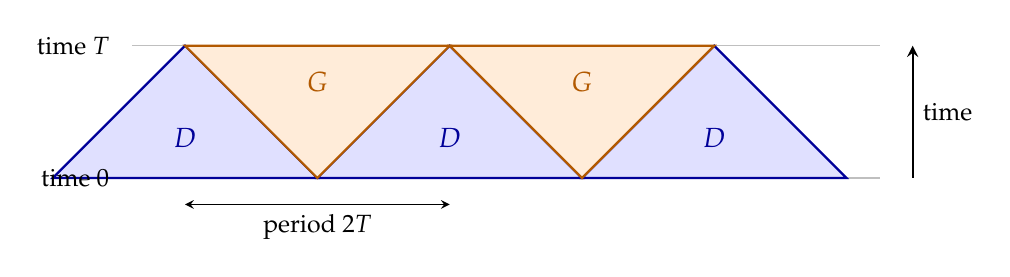
\begin{tikzpicture}[x=0.42cm,y=0.42cm,>=stealth]
\draw[gray!50] (-1.6,0) -- (21,0);
\draw[gray!50] (-1.6,4) -- (21,4);
\foreach \c in {0,8,16}{
  \fill[blue!12] (\c-4,0) -- (\c+4,0) -- (\c,4) -- cycle;
  \draw[blue!60!black,thick] (\c-4,0) -- (\c+4,0) -- (\c,4) -- cycle;
  \node[blue!60!black] at (\c,1.2) {$D$};
}
\foreach \m in {4,12}{
  \fill[orange!15] (\m,0) -- (\m+4,4) -- (\m-4,4) -- cycle;
  \draw[orange!70!black,thick] (\m,0) -- (\m+4,4) -- (\m-4,4) -- cycle;
  \node[orange!70!black] at (\m,2.9) {$G$};
}
\node[left] at (-2.0,0) {\small time $0$};
\node[left] at (-2.0,4) {\small time $T$};
\draw[<->] (0,-0.8) -- (8,-0.8) node[midway,below]{\small period $2T$};
\draw[->,thick] (22,0) -- (22,4) node[midway,right]{\small time};
\end{tikzpicture}
\caption{One slab of height $T$. Shrinking tiles $D_j$ (triangles with base on the initial row) and expanding gaps $G_j$ (triangles with apex on the initial row) partition the slab. A tile is sampled from its initial word; a gap from its initial word and the histories of its two lateral tiles. Different tiles, gaps and slabs use independent seeds.}
\label{fig:tiles}
\end{figure}

\subsection{Clipping a tile sampler to a finite volume}

\begin{lemma}[Clipped sampler]
\label{lem:clip}
Fix a finite space--time region $V$, an exterior history $\tau$, and a row below $V$ from which the forward process in $V$ starts. Sample the sites of $V$ in increasing time with the ordinary transition factors, exterior parents fixed to $\tau$, as follows: within each slab use an original table on every tile or gap wholly contained in $V$, and independent basic local maps, drawn chronologically, on every tile or gap cut by the boundary of $V$; generate the cut shrinking parts before the cut gap parts. This samples the exact forward law in $V$ with exterior $\tau$, and all seeds keep their original independent product law.
\end{lemma}

\begin{proof}
Clipping removes update sites and replaces their values, where needed, by the fixed exterior values; it creates no new dependency. A cut shrinking part depends only on the initial row and its own fresh maps; a complete shrinking table has the correct history law for its supplied initial word by \ref{B1}, and a cut part has the correct law by chronological generation. When a gap is reached, every lateral input has already been generated or is fixed outside $V$, and is independent of the gap's fresh seed; a complete gap table has the correct conditional history law for that record by \ref{B2}, and a cut gap again has the correct law chronologically. The conditional densities multiply to the product of the incoming factors of the sites of $V$, which chronological summation shows to be normalized. The procedure evaluates independent seeds at inputs and never conditions a seed on an imposed output, so the product law of the seeds is unchanged.
\end{proof}

The last sentence is the point. Sampling an unrestricted history and then conditioning its outer shell to equal $\tau$ would in general destroy the independence of the seeds; the lemma constructs the finite law directly. Only finitely many shapes of cut parts occur, so their dependence radii are uniformly bounded. Enlarge $A$ once and for all so that it controls every clipped sampler as well as the unrestricted tables, and so that $A\ge T$.

% =====================================================================
\section{The cap comparison}
\label{sec:cap}
% =====================================================================

This section proves the estimate that removes an arbitrary future boundary. It is stated for a single root site and, in \cref{lem:root} below, for a bounded initial footprint; the second form is used for whole tiles in \cref{sec:wsm}.

\subsection{Coarse cells and bad markers}
\label{sec:cells}

Group $m$ small slabs into a large slab of height $H=mT$. Choose a cell width $B$, a multiple of the period $2T$, with $B\ge(m+2)A$, and take the smallest such; thus $B=O(m)$ as $m$ grows, with $T$ and $A$ fixed. Let $C_k=[kB,(k+1)B-1]\cap\Z$. In large slab $j$ call the \emph{marker} $(j,k)$ \emph{bad} if the terminal word of the large slab on $C_k$, under the unrestricted table flow, is not constant as a function of the input row of that large slab. By \eqref{eq:B4} and a union bound over the $B$ sites of the cell,
\begin{equation}
\Prob\bigl((j,k)\ \text{is bad}\bigr)\;\le\;p_m\;:=\;B\,C_Be^{-d_Bm}.
\label{eq:pm}
\end{equation}
Finite locality supplies an integer $R_0\ge1$, \emph{independent of $m$}, such that the input support and the seed support of the terminal word on $C_k$ lie in the cells $k-R_0,\dots,k+R_0$: the word is a composition of $m$ slab maps of radius at most $A$, which span at most $mA\le B$ sites horizontally. Let $U_{j,k}$ be a deterministic set of seeds containing the whole dependence support of that word, chosen so that the same bound holds for clipped samplers, and so that changing a seed of $U_{j,k}$ can directly affect only terminal cells within $2R_0$ of $k$. Within one large slab, $U_{j,k}$ and $U_{j,k'}$ are disjoint when $|k-k'|>2R_0$; different large slabs use disjoint seeds. Set
\begin{equation}
D=2R_0+1,\qquad R=3R_0,\qquad \Delta=2(2R+1),\qquad \hatD=\Delta+2.
\label{eq:constants}
\end{equation}
The number $D$ is a spacing at which markers of one slab have disjoint seeds; $R$ bounds the horizontal spread of influence from one large slab to the next, counted in cells; $\Delta$ bounds the degree of the graph on markers used in \cref{sec:entropy}; the $+2$ in $\hatD$ allows horizontal edges between consecutive root cells.

\subsection{Expanding volumes and the cap identity}
\label{sec:capidentity}

Consider first the root $v=(0,0)$ and, for $n\ge1$, the region
\begin{equation}
V_n\;=\;\{v\}\cup\bigl\{(x,t):1\le t\le nH,\ |x|\le W+ct\bigr\},
\label{eq:Vn}
\end{equation}
with outward integer rounding, where the buffer $W$ and the speed $c\ge1$ are fixed once $m$ is fixed.

\begin{figure}[t]
\centering
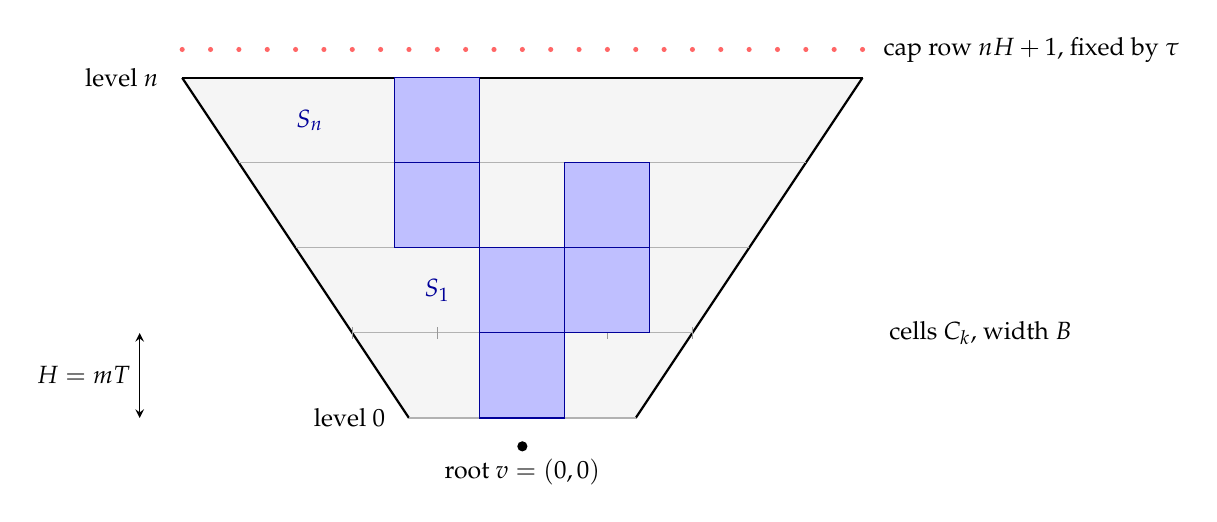
\begin{tikzpicture}[x=0.36cm,y=0.36cm,>=stealth]
% expanding volume
\fill[gray!8] (-4,1) -- (4,1) -- (12,13) -- (-12,13) -- cycle;
\draw[thick] (-4,1) -- (-12,13);
\draw[thick] (4,1) -- (12,13);
\draw[thick] (-4,1) -- (4,1);
% large slab boundaries
\foreach \t in {4,7,10,13}{ \draw[gray!60] ({-4-8*(\t-1)/12},\t) -- ({4+8*(\t-1)/12},\t); }
\draw[thick] (-12,13) -- (12,13);
% root
\fill (0,0) circle (0.18);
\node[below] at (0,-0.1) {\small root $v=(0,0)$};
\draw[gray!60] (-4,1) -- (4,1);
% cap row
\foreach \x in {-12,-11,...,12}{ \fill[red!60] (\x,14) circle (0.09); }
\node[right] at (12.4,14) {\small cap row $nH+1$, fixed by $\tau$};
% cells ticks on slab 4 boundary
\foreach \x in {-6,-3,0,3,6}{ \draw[gray!80] (\x,3.8) -- (\x,4.2); }
\node[right] at (12.6,4) {\small cells $C_k$, width $B$};
% cluster of bad markers
\fill[blue!25] (-1.5,1) rectangle (1.5,4);
\fill[blue!25] (-1.5,4) rectangle (1.5,7);
\fill[blue!25] (1.5,4) rectangle (4.5,7);
\fill[blue!25] (1.5,7) rectangle (4.5,10);
\fill[blue!25] (-4.5,7) rectangle (-1.5,10);
\fill[blue!25] (-4.5,10) rectangle (-1.5,13);
\draw[blue!60!black] (-1.5,1) rectangle (1.5,4);
\draw[blue!60!black] (-1.5,4) rectangle (1.5,7);
\draw[blue!60!black] (1.5,4) rectangle (4.5,7);
\draw[blue!60!black] (1.5,7) rectangle (4.5,10);
\draw[blue!60!black] (-4.5,7) rectangle (-1.5,10);
\draw[blue!60!black] (-4.5,10) rectangle (-1.5,13);
\node[blue!60!black] at (-7.5,11.5) {\small $S_n$};
\node[blue!60!black] at (-3,5.5) {\small $S_1$};
% labels
\node[left] at (-12.5,13) {\small level $n$};
\node[left] at (-4.5,1) {\small level $0$};
\draw[<->] (-13.5,1) -- (-13.5,4) node[midway,left]{\small $H=mT$};
\end{tikzpicture}
\caption{The expanding volume $V_n$ and the cap. The root influences the terminal row only through the reached cluster $S_1,\dots,S_n$ of bad markers (shaded), which starts at the root cell and spreads by at most $R$ cells per large slab. The cap factors (red) tilt the forward law by at most $e^{\beta}$ per changed terminal spin, so the tilt costs at most $e^{b|S_n|}$, while the probability that a candidate cluster is bad is at most $p_m^{M/D}$ with $M$ its total size. In one dimension $M\ge |S_n|H_n/(2R+1)$, and the logarithm wins.}
\label{fig:cap}
\end{figure} The first positive row of $V_n$ contains every child of $v$. We choose $W$ and $c$ large enough that every marker cone used below lies in complete tiles: if the root cells have indices in $[-s_*,s_*]$, every cell reached at level $j$ by the clusters of \cref{sec:splice} has $|k|\le s_*+Rj$, and all its relevant seed footprints, input supports and splice neighbourhoods lie horizontally within $|x|\le(s_*+Rj+4R_0+4)B+4A$ during that large slab. It suffices, for instance, to take integers
\begin{equation}
W\;\ge\;(s_*+R+4R_0+10)B+10A,\qquad c\;\ge\;2+\frac{(R+4R_0+10)B}{H}+\frac{10A}{T}.
\label{eq:Wc}
\end{equation}
At the bottom of large slab $j\ge2$ the half-width $W+c(j-1)H$ already exceeds the displayed support bound; the first large slab reads its arbitrary complete initial row. The margins contain entire tiles, not only their anchors, so only complete interior tiles are ever resampled.

Because the sides of $V_n$ expand at speed at least one, an exterior site at a time $1,\dots,nH$ has no interior parent: its parents are at horizontal distance at most one, hence beyond the half-width of the preceding row. The only exterior children of interior sites are therefore in the \emph{cap}, the row $nH+1$. Fix the exterior $\tau$. For $a\in\A$ let $X^a$ be the forward process in $V_n\setminus\{v\}$ with $\sigma_v=a$, started from the row $0$ that equals $\tau$ off $v$, sampled by \cref{lem:clip}, and let $X^a_{nH}$ be its terminal row. Direct factorization of \eqref{eq:spec} gives the exact identity
\begin{equation}
\gamma^\tau_{V_n}(\sigma_v=a)\;=\;\frac{p(a\mid\tau_{\Ue(v)})\,Z_a}{\sum_b p(b\mid\tau_{\Ue(v)})\,Z_b},\qquad Z_a=\E\,h\bigl(X^a_{nH}\bigr),
\label{eq:capidentity}
\end{equation}
where $h$ is the product of the transition factors of the cap sites, evaluated with their cap values from $\tau$ and their parents in the terminal row. Every $Z_a$ is positive. There is no omitted boundary-dependent normalization in \eqref{eq:capidentity}: the interior incoming factors form a normalized forward law, and $h$ contains all remaining factors touching $V_n$.

Put
\begin{equation}
K=\max_{b,u,u'}\frac{p(b\mid u)}{p(b\mid u')},\qquad\beta=3\log K.
\label{eq:K}
\end{equation}
Each terminal spin is a parent of at most three cap sites, so for terminal rows $z,z'$ agreeing outside the volume,
\begin{equation}
h(z)\;\le\;h(z')\,\exp\bigl\{\beta\,\dH(z,z')\bigr\},
\label{eq:lipschitz}
\end{equation}
with $\dH$ the Hamming distance. This charges for the number of changed terminal spins, not for the width of the cap.

\subsection{The deterministic splice}
\label{sec:splice}

Let $S_0$ be a fixed nonempty interval of root cells; the singleton application has $S_0=\{0\}$, and $|S_0|$ stays bounded by a fixed constant throughout. For a realization $x$ of the seed field define the \emph{reached cluster}
\begin{equation}
S_j(x)\;=\;\bigl\{k:\ \dist(k,S_{j-1}(x))\le R,\ (j,k)\ \text{is bad in }x\bigr\},\qquad 1\le j\le n.
\label{eq:reached}
\end{equation}
Once a level is empty, all later levels are empty. The law of the cluster depends only on the seeds, not on the sampled spins or on the exterior history.

\begin{lemma}[Seed splice]
\label{lem:splice}
Fix $x$ and its reached cluster $S=(S_0,\dots,S_n)$. Replace the seeds in
\[
U(S)=\bigcup_{j=1}^n\bigcup_{k\in S_j}U_{j,k}
\]
arbitrarily, obtaining $y$. Run the forward samplers of \cref{lem:clip} with $x$ and with $y$ from the same initial row and exterior. Their terminal rows at level $j$ differ only in cells within distance $2R_0$ of $S_j$. In particular, with $d=|S_n|$,
\begin{equation}
\dH\bigl(X_{nH}(x),X_{nH}(y)\bigr)\;\le\;B(4R_0+1)\,d.
\label{eq:splicebound}
\end{equation}
With the same seeds $x$, two initial rows that differ only in $S_0$ have identical cap rows whenever $S_n=\varnothing$.
\end{lemma}

\begin{proof}
Induct over large slabs. A terminal word at level $j$ that reads a replaced seed directly has index within $2R_0$ of some cell of $S_j$, by the support bounds. Otherwise its seed cone is unchanged. If its word nevertheless changes, some input cell at level $j-1$ changed; by the inductive hypothesis that input lies within $2R_0$ of $S_{j-1}$, so the terminal cell is within $R_0+2R_0=R$ of $S_{j-1}$ and is a candidate in \eqref{eq:reached}. Its cone lies in complete tiles by \eqref{eq:Wc}. If its marker were good, the whole terminal word would be constant over all input rows, which is incompatible with a changed word under unchanged cone seeds; so the marker is bad and the cell belongs to $S_j$. These two cases prove the induction and \eqref{eq:splicebound}, since each of the $d$ terminal cells of $S_n$ accounts for at most $4R_0+1$ cells of width $B$. For two initial rows supported on $S_0$ there are no seed replacements; the same induction starts with the disagreements in $S_0$, and if $S_n$ is empty there is no terminal disagreement.
\end{proof}

No property of the replacement seeds is asserted. A replacement can change a neighbouring good marker, but all its direct effects are inside the paid $2R_0$ neighbourhood.

\subsection{Resampling at a fixed cluster}
\label{sec:resample}

Fix a deterministic candidate cluster $S=(S_0,\dots,S_n)$ and let $x'$ be an independent copy of the product seed field. Define the hybrid field
\begin{equation}
y_z=\begin{cases}x'_z,& z\in U(S),\\ x_z,& z\notin U(S).\end{cases}
\label{eq:hybrid}
\end{equation}
Let $\mathcal B_S$ be the event that every nonroot marker listed in $S$ is bad in $x$. It depends only on $x|_{U(S)}$. The hybrid $y$ depends only on $x|_{U(S)^c}$ and $x'|_{U(S)}$; it therefore has the original product law and is independent of $\mathcal B_S$. The exact-cluster event $\{S(x)=S\}$ is contained in $\mathcal B_S$ but need not be independent of $y$.

Let $M=\sum_{j=1}^n|S_j|$, $d=|S_n|$ and $b=\beta B(4R_0+1)$. For a fixed root value $a$ the splice bound \eqref{eq:splicebound} together with \eqref{eq:lipschitz} holds for every $x'$ on $\{S(x)=S\}$, so
\begin{equation}
\begin{aligned}
\E_x\bigl[\mathbf 1_{\{S(x)=S\}}\,h(X^a_{nH}(x))\bigr]
&\;\le\;e^{bd}\,\E_{x,x'}\bigl[\mathbf 1_{\{S(x)=S\}}\,h(X^a_{nH}(y))\bigr]\\
&\;\le\;e^{bd}\,\E_{x,x'}\bigl[\mathbf 1_{\mathcal B_S}\,h(X^a_{nH}(y))\bigr]
\;=\;e^{bd}\,\Prob(\mathcal B_S)\,Z_a.
\end{aligned}
\label{eq:resample}
\end{equation}
The last equality uses the original law of $y$ and its independence from $\mathcal B_S$; division by the same $Z_a$ that appears in \eqref{eq:capidentity} is thus justified. Choose a residue class of cell indices modulo $D$ containing at least $M/D$ of the listed nonroot vertices; their seed sets are pairwise disjoint within each slab and different slabs are independent, so $\Prob(\mathcal B_S)\le p_m^{M/D}$ and
\begin{equation}
\frac{\E\bigl[\mathbf 1_{\{S(x)=S\}}\,h(X^a_{nH})\bigr]}{Z_a}\;\le\;e^{bd}\,p_m^{M/D}.
\label{eq:fixedS}
\end{equation}
This calculation is for a fixed candidate. Resampling a random set and asserting independence without the fixed-set calculation would not establish \eqref{eq:fixedS}.

\subsection{Cluster entropy and the harmonic gain}
\label{sec:entropy}

Consider the graph on vertices $(j,k)$ with an edge between $(j,k)$ and $(j+1,k')$ whenever $|k-k'|\le R$; its maximum degree is $\Delta$. Add horizontal edges between consecutive cells of the root interval $S_0$; the degree is then at most $\hatD$, and the root interval together with any reached cluster is connected. A deterministic spanning tree and a depth-first walk starting at the leftmost root cell recover a candidate with $M$ nonroot vertices by a walk of length $2(M+|S_0|-1)$, so the number of candidates with $M$ nonroot vertices is at most
\begin{equation}
C_{\mathrm{root}}\,\hatD^{\,2M},\qquad C_{\mathrm{root}}=\hatD^{\,2(|S_0|-1)}.
\label{eq:count}
\end{equation}
Counting all connected sets overcounts the reached clusters, which is harmless. A uniformly bounded root interval changes only the prefactor.

Now suppose $d=|S_n|>0$. Then there is a vertex at every positive level, so $M\ge n$. For $\ell=0,\dots,n-1$ every terminal vertex has an ancestor at level $n-\ell$, and an ancestor can reach at most $2R\ell+1$ distinct terminal cells, whatever the splitting and merging of paths. Hence
\begin{equation}
|S_{n-\ell}|\;\ge\;\frac{d}{2R\ell+1},\qquad M\;\ge\;d\sum_{\ell=0}^{n-1}\frac1{2R\ell+1}\;\ge\;\frac{d\,H_n}{2R+1},\qquad H_n=\sum_{j=1}^n\frac1j.
\label{eq:harmonic}
\end{equation}
This is the one-dimensional gain: it counts possible terminal endpoints, not paths, and in $d\ge2$ spatial dimensions the corresponding sum $\sum_\ell(2R\ell+1)^{-d}$ would be bounded.

Since $p_m$ decays exponentially in $m$ while $R_0$ and hence $D,\Delta,\hatD$ are fixed, choose $m$ once and for all so that
\begin{equation}
\tau_*\;:=\;e\,\hatD^{\,2}\,p_m^{1/D}\;<\;1.
\label{eq:taustar}
\end{equation}
With that $m$ fixed, take $n_0$ such that $H_{n_0}\ge b(2R+1)$. For $n\ge n_0$ and every candidate with $S_n\neq\varnothing$, \eqref{eq:harmonic} gives $e^{bd}\le e^M$, and summing \eqref{eq:fixedS} over candidates with \eqref{eq:count} and $M\ge n$ gives
\begin{equation}
\frac{\E\bigl[\mathbf 1_{\{S_n\neq\varnothing\}}\,h(X^a_{nH})\bigr]}{Z_a}\;\le\;C_{\mathrm{root}}\sum_{M\ge n}\tau_*^M\;=\;\frac{C_{\mathrm{root}}\,\tau_*^{\,n}}{1-\tau_*}\;=:\;\delta_n.
\label{eq:capbound}
\end{equation}
The reached cluster is thus exponentially unlikely under the actual, cap-tilted law. We have not claimed that the tilted law has independent seeds; the comparison went through the fixed-cluster resampling.

\subsection{Common extinction and the root comparison}
\label{sec:extinction}

On $\{S_n=\varnothing\}$ \cref{lem:splice} makes the cap row identical for every root value, so the common contribution $Z_0=\E[\mathbf 1_{\{S_n=\varnothing\}}h(X^a_{nH})]$ does not depend on $a$. Write $Z_a=Z_0+R_a$ with $R_a\ge0$; \eqref{eq:capbound} says $R_a\le\delta_nZ_a$ for $n\ge n_0$. More generally, let $w$ be any probability mass function on $\A$ and $\bar Z=\sum_aw(a)Z_a$, $\bar R=\sum_aw(a)R_a$. Then
\begin{equation}
\frac{w(a)Z_a}{\bar Z}\;=\;\frac{Z_0}{\bar Z}\,w(a)\;+\;\frac{\bar R}{\bar Z}\cdot\frac{w(a)R_a}{\bar R},\qquad \frac{\bar R}{\bar Z}\le\delta_n,
\label{eq:mixture}
\end{equation}
with the second term omitted when $\bar R=0$: the law $w(\cdot)Z_\cdot/\bar Z$ is a mixture of $w$ and another law with mixing weight at most $\delta_n$, so its total variation distance from $w$ is at most $\delta_n$. This also shows directly why a very small partition function causes no loss.

The argument remains valid when, conditional on $a$, the initial row inside a fixed finite footprint has any normalized law $\pi_a$ and the row outside the footprint is fixed: sample that initial row independently of the future seeds and include its expectation in $Z_a$. For a fixed sampled initial row the splice calculation is unchanged, and averaging preserves \eqref{eq:resample}. On extinction the cap row is the same for every assignment of the footprint, so the law $\pi_a$ integrates to one and the common contribution remains independent of $a$. This is the form used for whole tiles. Absorbing the finitely many $n<n_0$ into a constant, we have proved:

\begin{lemma}[Uniform root comparison]
\label{lem:root}
There are $C_0<\infty$ and $s\in(0,1)$ such that for every $n\ge1$ and every exterior history $\tau$,
\begin{equation}
\dtv\bigl((\gamma^\tau_{V_n})_v,\ p(\,\cdot\mid\tau_{\Ue(v)})\bigr)\;\le\;\min\{1,\,C_0s^n\}.
\label{eq:root}
\end{equation}
The same bound, with constants enlarged uniformly over finitely many footprint types, holds for a root consisting of a uniformly bounded initial footprint carrying any normalized law, in the sense of \eqref{eq:mixture}.
\end{lemma}

% =====================================================================
\section{Every DLR state is the stationary trajectory}
\label{sec:dlr}
% =====================================================================

Let $\nu$ be an arbitrary DLR state. For $v=(x,t)$ let $\mathcal F_v$ be the $\sigma$-field generated by all spins at times strictly below $t$ and by the other spins of row $t$. The translated volume $v+V_n$ of \eqref{eq:Vn} contains only $v$ in row $t$ and only future spins otherwise, so $\mathcal F_v$ is contained in the exterior $\sigma$-field of $v+V_n$. The DLR equation and the tower property give
\[
\nu(\sigma_v=a\mid\mathcal F_v)\;=\;\E_\nu\bigl[\gamma^\sigma_{v+V_n}(\sigma_v=a)\,\big|\,\mathcal F_v\bigr].
\]
The target $p(a\mid\sigma_{\Ue(v)})$ is $\mathcal F_v$-measurable, and \eqref{eq:root} is uniform in the exterior. Letting $n\to\infty$,
\begin{equation}
\nu(\sigma_v=a\mid\mathcal F_v)\;=\;p(a\mid\sigma_{\Ue(v)})\qquad\nu\text{-almost surely}.
\label{eq:onesite}
\end{equation}
No limiting exterior $\sigma$-field needs to be identified.

Let $\mathcal P_t$ be the $\sigma$-field of the strict past of row $t$. For distinct sites $x_1,\dots,x_k$ of row $t$, condition the product of their indicators first on $\mathcal F_{(x_1,t)}$: the other indicators are measurable there, and the first is replaced by its prescribed factor, which is $\mathcal P_t$-measurable. Repeating for each site,
\begin{equation}
\nu\bigl(\sigma_{x_j,t}=a_j,\ 1\le j\le k\,\big|\,\mathcal P_t\bigr)\;=\;\prod_{j=1}^kp\bigl(a_j\,\big|\,\sigma_{\Ue(x_j,t)}\bigr).
\label{eq:row}
\end{equation}
Finite cylinders determine the row law, so under $\nu$ every row is obtained from the preceding one by the PCA kernel: $\nu$ is a two-sided PCA trajectory, at this stage possibly an arbitrary entrance law rather than a stationary one.

Uniform ergodicity identifies the entrance law. Fix a finite space--time cylinder $E$ with earliest time $t_0$, and let $I$ be the finite set of sites of row $t_0$ from which all spins of $E$ are generated, by finite propagation. Under any entrance law the row at time $-N$ is some probability law, and \eqref{eq:uee} makes its marginal at row $t_0$ on $I$ converge to $\mu_I$ uniformly in that earlier law. Applying the same forward kernel from $I$ to $E$ cannot increase total variation, so letting $N\to\infty$ identifies the $E$-marginal of $\nu$ with that of the stationary trajectory. Hence every DLR state equals $\ba$. Existence follows from compactness of $\A^{\Z^2}$ and the continuity of the positive finite-range specification, or directly from \cref{lem:halfspace}. Uniqueness implies invariance under every space--time translation, because translates obey the same specification. This proves the uniqueness assertion of \cref{thm:main}.

% =====================================================================
\section{Weak mixing in arbitrary volumes, and clustering}
\label{sec:wsm}
% =====================================================================

The singleton comparison proves uniqueness, but weak mixing from bare exponential ergodicity needs one more step, because there may be no successful basic-map representation (\cref{rem:berard22}). We therefore compare an entire tile with its forward history law and couple with the independent history tables themselves.

\subsection{Whole-tile roots}

For a tile or gap $Q$ of a small slab, write $I_Q$ for its input record in the sense of \ref{B2}, and $\mathcal G_Q(\cdot\mid I_Q)$ for the law of its complete history under the normalized forward dynamics given that record.

\begin{lemma}[Whole-tile comparison]
\label{lem:tile}
There are $C_1<\infty$ and $s_1\in(0,1)$ such that for every tile or gap $Q$ and every $n\ge1$ there is a finite comparison volume $V_{Q,n}\supset Q$, lying in the slab of $Q$ and the slabs above it, with
\begin{equation}
\dtv\bigl((\gamma^\tau_{V_{Q,n}})_Q,\ \mathcal G_Q(\cdot\mid I_Q(\tau))\bigr)\;\le\;C_1s_1^{\,n}
\label{eq:tile}
\end{equation}
uniformly in the exterior history $\tau$. The diameter of $V_{Q,n}$ and its displacement from $Q$ are at most $a_0+a_1n$ for fixed constants. In the slab of $Q$, $V_{Q,n}$ consists of $Q$ and its two adjacent gaps when $Q$ is a shrinking tile, and of $Q$ alone when $Q$ is a gap.
\end{lemma}

\begin{proof}
Suppose first $Q=D_j$ is a shrinking tile, and put $W_Q=D_j\cup G_{j-1}\cup G_j$ in its slab. The neighbouring shrinking tiles are parent-closed, so no update in them reads $W_Q$; every outgoing arrow from $D_j$ within the slab enters one of the two included gaps; a gap has no outgoing arrow to another tile at a later time of the same slab. Hence every outgoing factor from $W_Q$ lies beyond the slab's terminal row.

Fix a complete history $q$ on $D_j$. Its incoming product is $\mathcal G_Q(q\mid I_Q)$, with $I_Q$ fixed outside the volume. Conditional on $q$, the two gaps carry their normalized forward laws, reading $q$ on one lateral side and the fixed exterior record on the other; this holds for arbitrary exterior records, whether or not they could occur in a sampled trajectory, because the normalization is an algebraic consequence of the stochastic factors. Append above the slab a buffered expanding tail of $n$ large slabs, as in \eqref{eq:Wc}, containing every child of the terminal footprint of $W_Q$ at its first time. The exact finite-volume marginal is
\begin{equation}
(\gamma^\tau_{V_{Q,n}})_Q(q)\;=\;\frac{\mathcal G_Q(q\mid I_Q)\,Z_q}{\sum_{q'}\mathcal G_Q(q'\mid I_Q)\,Z_{q'}},
\label{eq:tileidentity}
\end{equation}
where $Z_q$ averages the final cap likelihood over the normalized gap histories and the normalized tail. At the tail's starting row all dependence on $q$ and on the gap histories is confined to the terminal footprint $W_Q(T)$, which has width at most $4T-1$ by \eqref{eq:tiles} and, since $B\ge T$, is covered by at most five consecutive coarse cells. The footprint form of \cref{lem:root} applies with these cells as $S_0$: the initial law of the footprint may depend on $q$ but is normalized and independent of the future seeds, and on extinction the cap row is identical for every assignment of the footprint, so the weighted common contribution to $Z_q$ is independent of $q$. Equations \eqref{eq:capbound}--\eqref{eq:mixture} with $w(q)=\mathcal G_Q(q\mid I_Q)$ prove \eqref{eq:tile}.

If $Q=G_j$ is a gap, take $W_Q=G_j$. Its entire initial and lateral record is exterior, and no arrow leaves it for a different tile of the slab; \eqref{eq:tileidentity} holds without auxiliary gaps, and the terminal footprint is again bounded. Finitely many tile types and residue classes give common constants; the initial pieces are fixed finite sets and the tails have width and height linear in $n$.
\end{proof}

\subsection{The joint coupling}

\begin{proposition}[Arbitrary-volume convergence]
\label{prop:wsm}
Under \eqref{eq:uee} and $r=1$, there are $C_*,c_*>0$ such that \eqref{eq:conv} and \eqref{eq:wsm} hold.
\end{proposition}

\begin{proof}
Let $\Lam$ be a finite volume and $\tau$ an exterior. Sample $\gamma^\tau_\Lam$ by a chain rule in this order: slabs in increasing time; within each slab, all intersections of $\Lam$ with shrinking tiles, then all intersections with gaps, in any fixed order within each family. These intersections partition the sites of $\Lam$. A cut tile needs no comparison estimate.

For a tile $Q$ wholly contained in $\Lam$, let $K_Q$ be the exact conditional law of its history given the previously exposed spins. If $V_{Q,n}\subset\Lam$, all previously exposed spins lie outside $V_{Q,n}$: for a shrinking tile, the only other sites of its slab in $V_{Q,n}$ are the two adjacent gaps, which have not been exposed; for a gap, $V_{Q,n}$ contains nothing else of its slab; and the rest of $V_{Q,n}$ lies in later slabs. Its input record $I_Q$ is exposed when $Q$ is processed. Specification consistency and the tower property give
\begin{equation}
\dtv\bigl(K_Q,\ \mathcal G_Q(\cdot\mid I^{\mathrm{actual}}_Q)\bigr)\;\le\;C_1s_1^{\,n},
\label{eq:KQ}
\end{equation}
a comparison of complete histories, not only of one-site marginals.

Construct a joint coupling as follows. Draw the history table $\mathcal V_Q$ of $Q$ independently of the whole joint past, evaluate it at $I^{\mathrm{actual}}_Q$ to obtain $Y_Q$, of law $\mathcal G_Q(\cdot\mid I^{\mathrm{actual}}_Q)$, choose a maximal coupling of that law with $K_Q$, and sample the actual Gibbs history of $Q$ from its conditional distribution given $Y_Q$. Averaging over the fresh seed gives exactly $K_Q$, so the Gibbs marginal is correct; the seed is neither altered nor reweighted, so the seeds retain their product law. The construction is conditional on the full joint past, not only on the actual Gibbs history, and its local mismatch probability is bounded by \eqref{eq:KQ}; different mismatches need not be independent.

Use these same tables to evolve a \emph{reference} PCA trajectory from its stationary row law at a time preceding all the finite dependence cones needed, that row drawn independently of all tables; draw further reference tables outside $\Lam$ independently, and at a cut tile keep the fresh reference table while sampling the actual Gibbs part by any exact conditional sampler. Working through a finite dependence hull avoids any sampling order on an infinite row. The reference has law $\ba$, because the tables have the original history laws and the product seed law.

Fix a target $x\in\Lam$ at distance $\delta=\dist(x,\Lam^c)$. Its backward tile-dependence cone through $n$ large slabs contains at most $b_0(n+1)^2$ small tiles, each within distance $b_1+b_2n$ of $x$, and \cref{lem:tile} puts every comparison template $V_{Q,n}$ of such a tile within distance $b_3+b_4n$ of $x$. Choose
\begin{equation}
n(\delta)=\max\Bigl\{0,\Bigl\lfloor\frac{\delta-b_3-1}{b_4}\Bigr\rfloor\Bigr\}.
\label{eq:ndelta}
\end{equation}
For $n(\delta)\ge1$ all these templates lie in $\Lam$ and all these tiles are complete; this uses only the distance to the complement, so it is valid in volumes with holes. By a union bound,
\begin{equation}
\Prob(\text{some mismatch in the cone})\;\le\;C_2\,(n(\delta)+1)^2\,s_1^{\,n(\delta)}.
\label{eq:mismatch}
\end{equation}
If there is no mismatch, the actual target is the unrestricted table-flow output applied to the actual bottom row of the cone, and the reference is the same flow applied to its own bottom row. For a target on a terminal row, \eqref{eq:B4} bounds the failure to coalesce by an exponential in $n(\delta)$; for a target inside the last small slab, its value is a function of a bounded number of sites of the preceding terminal row and of the last slab's tables, and a union bound over those sites gives the same with changed constants. Hence
\begin{equation}
\Prob\bigl(\sigma^{\mathrm{actual}}_x\neq\sigma^{\mathrm{reference}}_x\bigr)\;\le\;C_2(n(\delta)+1)^2s_1^{\,n(\delta)}+C_3e^{-c_3n(\delta)},
\label{eq:target}
\end{equation}
and the trivial bound one when $n(\delta)=0$. The coalescence estimate has not been conditioned on successful local matches: the two failure events are union-bounded under the unaltered product law of the tables. The construction is one joint coupling for all targets, and $n(\delta)$ grows linearly in $\delta$, so the polynomial factor is absorbed into an exponential. A union over $x\in E$ proves \eqref{eq:conv}, and the triangle inequality between two exteriors proves \eqref{eq:wsm}.
\end{proof}

\begin{remark}[A simpler final coupling under a fixed-pair certificate]
\label{rem:simpler}
If \eqref{eq:fixed-pair} is available, the whole-tile step can be replaced by a site-by-site argument after \cref{lem:root}. Sample the Gibbs spins in increasing time with a fixed order inside each row; when $z+V_n\subset\Lam$, every previously exposed spin lies outside $z+V_n$, so the chain-rule conditional $K_z$ satisfies $\dtv(K_z,p(\cdot\mid\text{actual parents}))\le C_0s^n$. Draw a fresh basic map independently of the joint past, evaluate it at the actual parents, couple maximally with $K_z$, and run a stationary reference with the same maps; the Gibbs marginal and the product law of the maps are both preserved. For a target at distance $\delta$, choose $n$ proportional to $\delta$ so that its depth-$nL$ cone and all comparison templates for the $O(n^2)$ updates in it lie in $\Lam$; the local mismatch probability is at most $Cn^2s^n$, and at the bottom of the cone the two exposed input rows are independent of the future maps, so \cref{prop:fixed-pair} bounds the native disagreement of the two outputs by $\alpha^n$. There is no conditioning on successful matches, which is why a fixed-pair certificate suffices here although the cap argument used all-input coalescence of the independent tile flow.
\end{remark}

\subsection{Clustering}

\begin{proposition}[Exponential clustering]
\label{prop:cluster}
Under \eqref{eq:uee} and $r=1$, the bound \eqref{eq:cluster} holds.
\end{proposition}

\begin{proof}
Approximate the stationary trajectory at each target by the tile construction started from a fixed deterministic row a finite number $m'$ of small slabs earlier. At terminal-row sites \eqref{eq:B4} bounds the approximation error by $C_Be^{-d_Bm'}$; at interior-slab sites the preceding-terminal-row argument of \cref{prop:wsm} changes only constants. The approximation at a target is a function of an independent-seed cone of diameter at most $a+bm'$. For finite supports $E,F$ use one common seed field and choose $m'$ with $2(a+bm')<\dist(E,F)$: the seed cones of the two collections are disjoint, so the approximating observables $f^{(m')},g^{(m')}$ are independent. If $\eps_E,\eps_F$ are the probabilities that some spin of the respective support is incorrectly approximated, then $\eps_E\le C|E|e^{-cm'}$, $\eps_F\le C|F|e^{-cm'}$, and since $|f-f^{(m')}|\le2\|f\|_\infty$ on the mismatch event and zero otherwise,
\[
|\Cov(f,g)|\;\le\;4\,\|f\|_\infty\|g\|_\infty\,(\eps_E+\eps_F).
\]
Take $m'$ proportional to the separation and enlarge the constant for the finitely many small separations. The stationary process and all approximations are coupled by starting the reference before the finitely many cones from an independent stationary row; alternatively the exponentially coalescing flow defines them directly from the infinite-past seed field.
\end{proof}

\subsection{Return to arbitrary radius}
\label{sec:blocking}

For a radius-$r$ PCA, group $r$ consecutive sites into one block. The blocked alphabet is $\A^r$ and the blocked radius is one; the single-block transition probability is the product of the $r$ original transition probabilities, strictly positive and normalized, and conditional independence between block updates is preserved. Estimate \eqref{eq:uee} transfers with a factor $r$. The blocked space--time potential is the original one regrouped, not a different interaction, and DLR states correspond under the invertible blocking.

To transfer the arbitrary-volume estimates, let $\Lam$ be an original finite volume and $\hat\Lam$ the blocked volume of its completely included spatial blocks. Condition on the spins of partially included blocks; the conditional law on $\hat\Lam$ is the blocked Gibbs kernel with the induced exterior. Apply its uniform estimate and integrate over the conditioned spins. A site at original distance $\delta$ from $\Lam^c$ has blocked distance at least $\delta/r-1$ from the complement of $\hat\Lam$; sites in partially included blocks have bounded original distance and are covered by enlarging the prefactor. A union bound over the blocks meeting $E$ proves \eqref{eq:conv} in original coordinates, and clustering transfers by the same fixed rescaling.

\begin{proof}[Proof of \cref{thm:main}, forward direction]
Assume \eqref{eq:uee}. Block to radius one by \cref{sec:blocking}. \Cref{sec:dlr} proves that $\ba$ is the only DLR state; \cref{prop:wsm} proves \eqref{eq:conv} and \eqref{eq:wsm}; \cref{prop:cluster} proves \eqref{eq:cluster}. The converse direction is \cref{prop:wsm-to-erg} below.
\end{proof}

% =====================================================================
\section{Converses in every dimension}
\label{sec:converse}
% =====================================================================

In this section the spatial lattice is $\Z^d$ for any $d\ge1$, with a finite alphabet, a finite neighbourhood and a strictly positive table.

\begin{proposition}[Weak mixing implies exponential ergodicity]
\label{prop:wsm-to-erg}
In every spatial dimension, \eqref{eq:wsm} implies \eqref{eq:uee}. For this implication it suffices to assume \eqref{eq:wsm} on rectangular space--time volumes.
\end{proposition}

\begin{proof}
Choose a stationary row law $\mu$ and its two-sided stationary trajectory $\ba$. Fix a finite $I\subset\Z^d$, a deterministic row $\eta$ and $t\ge1$, and put
\[
\Lam_\varrho=[-\varrho,\varrho]^d\times\{1,\dots,2t\},\qquad E=I\times\{t\},\qquad M=\max_{x\in I}\|x\|_\infty.
\]
By \cref{lem:halfspace}, both $(\nu^\eta)_E$ and $\ba_E$ are mixtures of the finite-volume kernels $(\gamma^\tau_{\Lam_\varrho})_E$ over their respective exterior distributions. Integrating \eqref{eq:wsm} against any coupling of these exterior laws, and using convexity of total variation,
\[
\dtv\bigl((P^t\eta)_I,\mu_I\bigr)\;\le\;C\,|I|\,e^{-c\min\{t,\ \varrho-M+1\}}.
\]
Let $\varrho\to\infty$. This is \eqref{eq:uee}, uniformly in $\eta$, and it implies uniqueness of the stationary law.
\end{proof}

\begin{theorem}[Uniqueness implies uniform local convergence]
\label{thm:qualitative}
In every spatial dimension, if the normalized space--time interaction has exactly one DLR state, then for every finite $I\subset\Z^d$,
\begin{equation}
\sup_\eta\ \dtv\bigl((P^t\eta)_I,\mu_I\bigr)\;\longrightarrow\;0\qquad(t\to\infty),
\label{eq:qualitative}
\end{equation}
where $\mu$ is the unique stationary row law. No rate is asserted.
\end{theorem}

\begin{proof}
Start with any stationary row law $\mu$; its trajectory law is DLR by \cref{lem:halfspace}. If \eqref{eq:qualitative} fails, there are a finite $I$, some $\delta>0$, times $t_n\to\infty$ and rows $\eta_n$ with $\dtv((P^{t_n}\eta_n)_I,\mu_I)\ge\delta$. Run the PCA from $\eta_n$ at time $-t_n$, fill the earlier past arbitrarily, and extract a weakly convergent subsequence of these measures on the compact space $\A^{\Z^{d+1}}$, with limit $\nu$. Every fixed finite region eventually lies strictly above the initial row, so \cref{lem:halfspace} gives its DLR identity for all large $n$; for a finite-range positive specification, a finite-volume kernel sends cylinder functions to continuous cylinder functions, so the integrated DLR identities, including multiplication by exterior cylinder functions, pass to the weak limit, and a monotone-class argument extends them to bounded measurable functions. Thus $\nu$ is DLR. Finite-alphabet marginal total variation is continuous under weak convergence, so the row-zero $I$-marginal of $\nu$ is at distance at least $\delta$ from $\mu_I$ and $\nu\neq\ba$, contradicting uniqueness. Uniform local convergence follows, and any other stationary law equals $\mu$ by integrating \eqref{eq:qualitative}.
\end{proof}

\begin{corollary}
\label{cor:nonerg}
In every dimension, a positive PCA that is not ergodic has a normalized space--time specification with more than one DLR state.
\end{corollary}

The second Gibbs state furnished by the compactness argument need not be stationary; the corollary does not produce two stationary row laws from non-ergodicity alone. Whether a non-ergodic positive PCA must have two stationary laws is itself open \cite{CM11}.

% =====================================================================
\section{Every dimension, no rate: the defect bound}
\label{sec:defect}
% =====================================================================

The converses of \cref{sec:converse} hold in every dimension but say nothing about which DLR states can exist beside the stationary trajectory when $d\ge2$. This section proves, in every dimension and with no rate, that the distance of any DLR state from the forward dynamics, measured by relative entropy, is a surface term. Most of the section is a few lines from that bound: the classical identification of translation-invariant Gibbs states with stationary laws, the fact that every \emph{uniformly recurrent} Gibbs state of an ergodic PCA is the stationary trajectory, and the unique ergodicity of the translation action on the simplex of Gibbs states. The only other input is Halawi's Baire-category argument that ergodic positive PCA are uniformly ergodic. The section depends only on \cref{sec:setting}, on the row equation \eqref{eq:row}, and on \cref{thm:qualitative}.

Throughout, the spatial lattice is $\Z^d$ with a finite neighbourhood $N$, and $p_-=\min_{a,u}p(a\mid u)>0$ is the least table entry. Order $\Z^{d+1}$ by time first and lexicographically within a row, and write $w\prec v$ for this translation-invariant order. The \emph{strict past} of $v$ is $H_v=\{w:w\prec v\}$ and $\mathcal P_v$ is the $\sigma$-field generated by $\sigma_{H_v}$, extending the notation $\mathcal P_t$ of \cref{sec:dlr} from rows to sites; the parents $\Ue(v)$ lie in $H_v$. For probability vectors $\alpha,\beta$ on $\A$ with $\beta$ strictly positive, $\mathrm{KL}(\alpha\,\|\,\beta)=\sum_a\alpha(a)\log\bigl(\alpha(a)/\beta(a)\bigr)\ge0$, with equality only when $\alpha=\beta$; the map $\alpha\mapsto\mathrm{KL}(\alpha\,\|\,\beta)$ is convex and continuous.

\subsection{The causal defect and the surface bound}

\begin{definition}[Causal defect]
\label{def:defect}
For a probability measure $\nu$ on $\A^{\Z^{d+1}}$ and a site $v$,
\begin{equation}
\kappa_v(\nu)\;=\;\E_\nu\,\mathrm{KL}\Bigl(\nu\bigl(\sigma_v\in\cdot\,\big|\,\mathcal P_v\bigr)\,\Big\|\,p\bigl(\cdot\,\big|\,\sigma_{\Ue(v)}\bigr)\Bigr)\;\in\;[0,\log(1/p_-)].
\label{eq:defect}
\end{equation}
\end{definition}

The defect measures how far the conditional law of a spin given its whole past is from the transition law read off its parents. It vanishes everywhere exactly for the trajectories of the PCA.

\begin{lemma}[Zero defect means trajectory]
\label{lem:zerodefect}
$\kappa_v(\nu)=0$ for every $v$ if and only if $\nu$ is a two-sided trajectory law of the PCA, that is, \eqref{eq:row} holds for every row.
\end{lemma}

\begin{proof}
$\kappa_v(\nu)=0$ means $\nu(\sigma_v=a\mid\mathcal P_v)=p(a\mid\sigma_{\Ue(v)})$ almost surely. Suppose this holds at every site and let $x_1\prec\dots\prec x_k$ be sites of row $t$. The $\sigma$-field generated by $\mathcal P_t$ and $\sigma_{x_1,t},\dots,\sigma_{x_{j-1},t}$ is contained in $\mathcal P_{(x_j,t)}$, so the tower property replaces the indicator of $\{\sigma_{x_j,t}=a_j\}$ by $p(a_j\mid\sigma_{\Ue(x_j,t)})$, which is $\mathcal P_t$-measurable; doing this for $j=k,k-1,\dots,1$ gives \eqref{eq:row}. Conversely, under a trajectory law \eqref{eq:row} gives, for $v=(x,t)$ and every finite set $F$ of sites of row $t$ preceding $v$, $\nu(\sigma_v=a\mid\mathcal P_t,\sigma_{F})=p(a\mid\sigma_{\Ue(v)})$; letting $F$ increase to all such sites and applying martingale convergence gives the same conditional law given $\mathcal P_v$, so $\kappa_v(\nu)=0$.
\end{proof}

\begin{theorem}[Surface defect bound]
\label{thm:defect}
Let $\nu$ be any DLR state of the normalized space--time interaction of a positive PCA on $\Z^d$, and let $\Lam\subset\Z^{d+1}$ be finite. Write $\partial_+\Lam=\{v\notin\Lam:\Ue(v)\cap\Lam\neq\varnothing\}$ for the exterior children of $\Lam$. Then
\begin{equation}
\sum_{v\in\Lam}\kappa_v(\nu)\;\le\;|\partial_+\Lam|\,\log(1/p_-).
\label{eq:surface}
\end{equation}
No invariance is assumed.
\end{theorem}

\begin{proof}
Fix an exterior configuration $\xi$. The product in \eqref{eq:spec} runs over the sites of $\Lam\cup\partial_+\Lam$, so
\[
\gamma^\xi_\Lam\;=\;\frac{\lambda\,B}{\lambda(B)},\qquad
\lambda(\omega)=\prod_{v\in\Lam}p\bigl((\omega\xi)_v\,\big|\,(\omega\xi)_{\Ue(v)}\bigr),\qquad
B(\omega)=\prod_{v\in\partial_+\Lam}p\bigl(\xi_v\,\big|\,(\omega\xi)_{\Ue(v)}\bigr).
\]
Here $\lambda$ is a probability measure on $\A^\Lam$: summing out the $\prec$-last site of $\Lam$ removes one factor, which sums to one because that site is a parent of no other site of $\Lam$, and induction does the rest. The same telescoping shows that under $\lambda$ the conditional law of $\omega_v$ given the sites of $\Lam$ preceding $v$ is $p(\cdot\mid(\omega\xi)_{\Ue(v)})$. Since $p_-^{|\partial_+\Lam|}\le B\le1$,
\[
\mathrm{KL}(\gamma^\xi_\Lam\,\|\,\lambda)\;=\;\int\log B\,d\gamma^\xi_\Lam-\log\lambda(B)\;\le\;|\partial_+\Lam|\log(1/p_-).
\]
Expand the left side by the chain rule along $\prec$: it is the sum over $v\in\Lam$ of the expected relative entropy of the conditional law of $\omega_v$ given the preceding sites of $\Lam$ under $\gamma^\xi_\Lam$ with respect to the same conditional law under $\lambda$, which is $p(\cdot\mid(\omega\xi)_{\Ue(v)})$. Now let $\xi=\sigma_{\Lam^c}$ be distributed under $\nu$. By the DLR equation $\gamma^{\sigma_{\Lam^c}}_\Lam$ is the conditional law of $\sigma_\Lam$ given $\sigma_{\Lam^c}$, so the $v$-th term of the chain rule, integrated over the exterior, becomes
$\E_\nu\,\mathrm{KL}\bigl(\nu(\sigma_v\in\cdot\mid\mathcal A_v)\,\|\,p(\cdot\mid\sigma_{\Ue(v)})\bigr)$ with $\mathcal A_v$ generated by $\sigma_{\Lam^c}$ and the spins of $\Lam$ preceding $v$. Since $H_v$ is contained in $\Lam^c$ together with the sites of $\Lam$ preceding $v$, we have $\mathcal P_v\subset\mathcal A_v$, and $p(\cdot\mid\sigma_{\Ue(v)})$ is $\mathcal P_v$-measurable. Conditional Jensen for the convex map $\alpha\mapsto\mathrm{KL}(\alpha\,\|\,\beta)$, with $\E[\nu(\sigma_v\in\cdot\mid\mathcal A_v)\mid\mathcal P_v]=\nu(\sigma_v\in\cdot\mid\mathcal P_v)$, bounds the $v$-th term below by $\kappa_v(\nu)$.
\end{proof}

For the box $\Lam_n=[-n,n]^{d+1}$ the exterior children lie within the range of $N$ of its lateral faces or just above its top row, so $|\partial_+\Lam_n|\le C_Nn^d$ while $|\Lam_n|\asymp n^{d+1}$:
\begin{equation}
\sup_{\nu\ \mathrm{DLR}}\ \sup_{w\in\Z^{d+1}}\ \frac1{|\Lam_n|}\sum_{v\in w+\Lam_n}\kappa_v(\nu)\;\le\;\frac{C_N\log(1/p_-)}{n}.
\label{eq:boxavg}
\end{equation}
The defect of a Gibbs state is therefore a boundary effect: it can be large at some sites, but not on a set of positive density.

\subsection{Translation-invariant, periodic and uniformly recurrent states}

Translations $\tau_w$, $w\in\Z^{d+1}$, act on configurations and on measures; since the order $\prec$ is translation invariant, $\kappa_{v+w}(\nu)=\kappa_v(\tau_w\nu)$ with the appropriate sign convention, which plays no role below. The specification is translation invariant, so translations act on the set $\mathcal G$ of DLR states, which is compact and convex in the weak topology.

\begin{corollary}[Periodic states are stationary trajectories]
\label{cor:gklm}
A DLR state invariant under a finite-index subgroup of $\Z^{d+1}$, in particular a translation-invariant one, is a two-sided trajectory law; if it is invariant under the time translation its row law is stationary. In particular the translation-invariant DLR states are exactly the trajectory laws of the translation-invariant stationary row laws, which is the correspondence of \cite{GKLM89}.
\end{corollary}

\begin{proof}
A subgroup of index $L$ contains $L\Z^{d+1}$. If $\nu$ is invariant under $L\Z^{d+1}$ then $v\mapsto\kappa_v(\nu)$ is $L$-periodic, so the averages in \eqref{eq:boxavg} converge to the average over one period cell, which is therefore $0$; as every term is nonnegative, $\kappa_v(\nu)=0$ for all $v$, and \cref{lem:zerodefect} applies. Time invariance of a trajectory law says that its row law is stationary. The converse direction is \cref{lem:halfspace}.
\end{proof}

A measure $\nu\in\mathcal G$ is \emph{uniformly recurrent} if for every weak neighbourhood $W$ of $\nu$ the set $\{w\in\Z^{d+1}:\tau_w\nu\in W\}$ is syndetic, that is, meets every translate of some finite box depending on $W$. Periodic states are uniformly recurrent, and so is every point of a minimal orbit closure; in fact uniform recurrence of $\nu$ is equivalent to minimality of its orbit closure, by the usual argument, and the property is shared by $\nu$ and all its translates.

\begin{lemma}[The defect is lower semicontinuous]
\label{lem:lsc}
On $\mathcal G$ with the weak topology, $\nu\mapsto\kappa_0(\nu)$ is a supremum of continuous functions, hence lower semicontinuous and Borel.
\end{lemma}

\begin{proof}
For $n$ large enough that $\Ue(0)\subset[-n,n]^{d+1}$, let $D_n=H_0\cap[-n,n]^{d+1}$ and $\kappa^{(n)}(\nu)=\E_\nu\mathrm{KL}\bigl(\nu(\sigma_0\in\cdot\mid\sigma_{D_n})\,\|\,p(\cdot\mid\sigma_{\Ue(0)})\bigr)$. Conditional Jensen, as in the proof of \cref{thm:defect}, makes $\kappa^{(n)}$ nondecreasing in $n$, and martingale convergence together with the boundedness and continuity of $\mathrm{KL}(\cdot\,\|\,\beta)$ for $\beta\ge p_-$ gives $\kappa^{(n)}\uparrow\kappa_0$. Finally $\kappa^{(n)}(\nu)=H_\nu(\sigma_{D_n})-H_\nu(\sigma_0,\sigma_{D_n})-\E_\nu\log p(\sigma_0\mid\sigma_{\Ue(0)})$, where $H_\nu$ is the Shannon entropy of a finite marginal: a continuous function of the marginal of $\nu$ on $\{0\}\cup D_n$.
\end{proof}

\begin{theorem}[Uniformly recurrent Gibbs states are trajectories]
\label{thm:recurrent}
Every uniformly recurrent DLR state of a positive PCA on $\Z^d$ is a two-sided trajectory law.
\end{theorem}

\begin{proof}
Suppose $\kappa_0(\nu)>\eps>0$. By \cref{lem:lsc} the set $W=\{\nu'\in\mathcal G:\kappa_0(\nu')>\eps\}$ is open, so the set $S$ of $w$ with $\kappa_w(\nu)>\eps$ is syndetic: it meets every translate of some finite box $Q_0$. A box $\Lam_n$ contains at least $c\,n^{d+1}$ disjoint translates of $Q_0$, so $\sum_{v\in\Lam_n}\kappa_v(\nu)\ge\eps\,c\,n^{d+1}$, which contradicts \eqref{eq:boxavg} for large $n$. Hence $\kappa_0(\nu)=0$. Every translate of $\nu$ is uniformly recurrent, so $\kappa_v(\nu)=0$ for every $v$, and \cref{lem:zerodefect} concludes.
\end{proof}

\subsection{Ergodic PCA}

The PCA is \emph{ergodic} if it has a stationary law $\mu$ with $\nu P^t\to\mu$ weakly for every initial law $\nu$, and \emph{uniformly ergodic} if moreover \eqref{eq:qualitative} holds, that is, the convergence is uniform in the initial row on every finite set of sites. Uniform exponential ergodicity implies uniform ergodicity, which implies ergodicity. For positive rates the last two notions coincide; the following argument is Halawi's \cite[Theorem~4.2.3 and Proposition~4.2.4]{Halawi22}, and we reproduce it because the thesis is not widely available.

\begin{proposition}[Ergodic positive PCA are uniformly ergodic]
\label{prop:halawi}
A strictly positive PCA on $\Z^d$ that is ergodic is uniformly ergodic.
\end{proposition}

\begin{proof}
Fix a finite $I$, a pattern $c\in\A^I$ and $\eps>0$, and for $m\ge1$ let $E_m$ be the set of rows $\eta$ with $|(P^t\eta)_I(c)-\mu_I(c)|\le\eps/2$ for all $t\ge m$. Each $\eta\mapsto(P^t\eta)_I(c)$ depends on finitely many coordinates of $\eta$, so $E_m$ is closed, and ergodicity applied to the deterministic rows says that the $E_m$ cover the compact space $\A^{\Z^d}$. By Baire's theorem some $E_m$ has nonempty interior, hence contains a cylinder $[\zeta_J]=\{\eta:\eta_J=\zeta_J\}$ with $J$ finite. By positivity, from any row the next row lies in $[\zeta_J]$ with probability at least $p_-^{|J|}$, so the first entrance time $T$ of the chain $(X_t)$ into $[\zeta_J]$ satisfies $\Prob(T>s)\le(1-p_-^{|J|})^s$ uniformly in the initial row. Fix $s$ and $t\ge m+s$. By the strong Markov property at the stopping time $T\wedge s$, $(P^t\eta)_I(c)=\E\bigl[(P^{\,t-T\wedge s}X_{T\wedge s})_I(c)\bigr]$. On $\{T\le s\}$ the row $X_T$ lies in $[\zeta_J]\subset E_m$ and $t-T\ge m$, so the integrand is within $\eps/2$ of $\mu_I(c)$; on $\{T>s\}$ it is within $1$. Hence, for every $\eta$,
\[
\bigl|(P^t\eta)_I(c)-\mu_I(c)\bigr|\;\le\;\frac\eps2+\Prob(T>s)\;\le\;\frac\eps2+(1-p_-^{|J|})^s.
\]
Choosing $s$ with $(1-p_-^{|J|})^s\le\eps/2$ and taking the finitely many patterns $c$ gives \eqref{eq:qualitative}.
\end{proof}

\begin{lemma}[Uniform ergodicity is uniqueness of the entrance law]
\label{lem:entrance}
For a positive PCA on $\Z^d$, with $\Delta(I,t)=\sup_{\eta,\zeta}\dtv\bigl((P^t\eta)_I,(P^t\zeta)_I\bigr)$, the following are equivalent:
\begin{enumerate}[label=\textup{(\roman*)}]
\item the PCA is uniformly ergodic;
\item $\Delta(I,t)\to0$ as $t\to\infty$ for every finite $I$;
\item the PCA has exactly one two-sided trajectory law.
\end{enumerate}
\end{lemma}

\begin{proof}
(i)$\Leftrightarrow$(ii) is the triangle inequality in one direction and integration of $\zeta$ against $\mu$ in the other. (ii)$\Rightarrow$(iii): two two-sided trajectory laws have row-$0$ laws of the form $\nu_{-s}P^s$ and $\nu'_{-s}P^s$ for every $s$, so their $I$-marginals at row $0$ are within $\Delta(I,s)\to0$ of each other; the same holds at every row, and a trajectory law is determined by its row laws and the kernel. (iii)$\Rightarrow$(ii): if $\Delta(I,t_n)\ge\delta$ along $t_n\to\infty$, with rows $\eta_n,\zeta_n$, run the PCA from $\eta_n$ and from $\zeta_n$ at time $-t_n$, fill the earlier rows deterministically, and extract weak limits along a common subsequence. Every fixed finite region eventually lies above the initial row, so the identities \eqref{eq:row}, integrated against finitely many past cylinders, hold for all large $n$ and pass to the limit, and a monotone-class argument gives \eqref{eq:row} for both limits: they are two-sided trajectory laws. Their row-$0$ marginals on $I$ are at distance at least $\delta$, contradicting (iii).
\end{proof}

\begin{remark}[Ergodicity of a rational positive PCA is $\Pi^0_2$]
\label{rem:pi2}
$(P^t\eta)_I$ depends on $\eta$ only through the sites within distance $t\max_{y\in N}\|y\|_\infty$ of $I$, and is a polynomial in the table entries, so $\Delta(I,t)$ is computable from a rational table. It is nonincreasing in $t$, because $(P^{t+1}\eta)_I$ is a mixture of the laws $(P^t\zeta)_I$ and total variation is convex. By \cref{lem:entrance}, uniform ergodicity is the statement $\forall I\,\forall k\,\exists t\ \Delta(I,t)<1/k$, and by \cref{prop:halawi} so is ergodicity: a $\Pi^0_2$ property of the table. We have not found this placement stated elsewhere.
\end{remark}

\begin{theorem}[The Gibbs simplex of an ergodic PCA]
\label{thm:simplex}
Let a strictly positive PCA on $\Z^d$ be ergodic, with stationary law $\mu$ and stationary trajectory law $\ba$, and let $\mathcal G$ be the set of DLR states of its normalized space--time interaction. Then:
\begin{enumerate}[label=(\roman*)]
\item\label{it:s1} $\ba$ is the only two-sided trajectory law and the only uniformly recurrent DLR state; in particular it is the only periodic DLR state;
\item\label{it:s2} $\delta_{\ba}$ is the only translation-invariant probability measure on $\mathcal G$; consequently, for every continuous $f$ on $\mathcal G$, $|\Lam_n|^{-1}\sum_{w\in\Lam_n}f(\tau_w\nu)\to f(\ba)$ uniformly in $\nu\in\mathcal G$;
\item\label{it:s3} $\ba$ is an extreme point of $\mathcal G$.
\end{enumerate}
Every DLR state other than $\ba$ therefore fails uniform recurrence: it has a neighbourhood whose return set under translation has arbitrarily large gaps.
\end{theorem}

\begin{proof}
\ref{it:s1} \Cref{prop:halawi} and \cref{lem:entrance} give the uniqueness of the trajectory law, and \cref{thm:recurrent} identifies every uniformly recurrent DLR state with it.

\ref{it:s2} Let $\varrho$ be a translation-invariant Borel probability measure on $\mathcal G$. By \cref{lem:lsc} the integrals below make sense, and invariance gives $\int\kappa_v\,d\varrho=\int\kappa_0\,d\varrho$ for every $v$. Integrating \eqref{eq:boxavg} against $\varrho$ yields $\int\kappa_0\,d\varrho\le C_N\log(1/p_-)/n$ for every $n$, so $\kappa_0=0$ $\varrho$-almost surely, hence $\kappa_v=0$ $\varrho$-almost surely for each of the countably many $v$, and \cref{lem:zerodefect} with \ref{it:s1} shows that $\varrho$-almost every $\nu$ equals $\ba$. Thus $\varrho=\delta_{\ba}$. If the averages of some continuous $f$ failed to converge uniformly, a sequence of empirical measures $|\Lam_{n_k}|^{-1}\sum_{w\in\Lam_{n_k}}\delta_{\tau_w\nu_k}$ would have a weak limit point that is translation invariant and different from $\delta_{\ba}$.

\ref{it:s3} By \cite[Theorem~7.26]{Georgii11} every DLR state has a unique representation $\nu=\int\nu'\,\varrho_\nu(d\nu')$ with $\varrho_\nu$ carried by the extreme points of $\mathcal G$. Translations map extreme points to extreme points and fix $\ba$, so uniqueness of the representation makes $\varrho_{\ba}$ translation invariant, whence $\varrho_{\ba}=\delta_{\ba}$ by \ref{it:s2}, that is, $\ba$ is extreme.
\end{proof}

\begin{corollary}[Finitely many phases]
\label{cor:finitephase}
If a strictly positive PCA on $\Z^d$ is ergodic and $\mathcal G$ has finitely many extreme points, then $\mathcal G=\{\ba\}$.
\end{corollary}

\begin{proof}
Let $K$ be the number of extreme points. By the Krein--Milman theorem $\mathcal G$ is their convex hull, and translations act on $\mathcal G$ by affine homeomorphisms, so they permute the extreme points. The translations in $L\Z^{d+1}$ with $L=\operatorname{lcm}(1,\dots,K)$ fix every extreme point and, being affine, every DLR state. By \cref{cor:gklm} every DLR state is then a trajectory law whose row laws $\nu_t$ satisfy $\nu_{t+1}=\nu_tP$ and $\nu_{t+L}=\nu_t$; ergodicity gives $\nu_t=\lim_k\nu_tP^{kL}=\mu$, so every DLR state is $\ba$.
\end{proof}

\begin{corollary}[All-DLR uniqueness in every dimension]
\label{cor:allDLR}
For a strictly positive PCA on $\Z^d$ the following are equivalent:
\begin{enumerate}[label=(\alph*)]
\item the normalized space--time interaction has exactly one DLR state;
\item the PCA is ergodic and every DLR state is uniformly recurrent.
\end{enumerate}
\end{corollary}

\begin{proof}
(a)$\Rightarrow$(b): \cref{thm:qualitative} gives uniform local convergence, hence ergodicity, and the unique DLR state is $\ba$, which is translation invariant and so uniformly recurrent. (b)$\Rightarrow$(a) is \cref{thm:simplex}\ref{it:s1}.
\end{proof}

\begin{remark}[What the defect bound does not exclude]
\label{rem:notexcluded}
\Cref{cor:allDLR} locates the gap in \cref{prob:higher} precisely: for an ergodic PCA in $d\ge2$, a second DLR state would have to be a boundary-selected state that is not uniformly recurrent, returning to a neighbourhood of itself only along a set of translations with arbitrarily large gaps. Equilibrium statistical mechanics knows such objects: for four-dimensional lattice gauge theories with a finite abelian group at weak coupling, Borgs \cite{Borgs84} proves that the translation-invariant equilibrium state is unique and constructs a second, non-invariant one, carried by a localized magnetic flux tube that starts and ends at infinity. In the opposite direction, Lebowitz and Mazel \cite{LM97} prove that in the Pirogov--Sinai regime uniqueness among translation-periodic Gibbs states implies global uniqueness. The space--time interaction of a positive PCA has zero pressure and no low-temperature structure, so neither the example nor the theorem transfers directly. In $d=1$ under exponential ergodicity such states are excluded by \cref{thm:main}, and in every dimension they are excluded under the hypotheses of \cref{thm:prefix}. For an ergodic PCA that is not exponentially ergodic the question is open: such PCA exist on $\Z^2$ (\cref{thm:critical}), and whether they exist on $\Z$ is part of \cref{prob:rate}.
\end{remark}

% =====================================================================
\section{Examples}
\label{sec:examples}
% =====================================================================

\subsection{Any rule at high noise}
\label{sec:highnoise}

Let $f\colon\A^{[-r,r]}\to\A$ be a deterministic rule and perturb it by uniform noise: with probability $1-\eps$ the update applies $f$, with probability $\eps$ it outputs a uniformly random symbol. The kernel is $p_\eps(a\mid u)=(1-\eps)\mathbf 1\{a=f(u)\}+\eps/|\A|$, strictly positive for $\eps>0$. Represent each update by $f$ with probability $1-\eps$ and by a fresh constant map with probability $\eps$. If the depth-$t$ composite map at the origin is nonconstant, tracing an essential input backwards yields a path of $t$ deterministic updates; there are at most $(2r+1)^t$ such paths, and the updates along a fixed path are independent because their times differ. Hence
\begin{equation}
q_t(\eps)\;\le\;\bigl[(2r+1)(1-\eps)\bigr]^t,
\label{eq:highnoise}
\end{equation}
which decays exponentially for $\eps>1-1/(2r+1)$. By \cref{prop:common-map} and \cref{thm:main}, every noisy rule at that noise has a unique space--time DLR state with exponential weak mixing. At $\eps=1$ every factor is constant and the unique DLR state is i.i.d.\ uniform. The path count behind \eqref{eq:highnoise} is the branching comparison that gives $p_c(N)\ge1/|N|$ for directed site percolation; Marcovici, Sablik and Taati prove uniform ergodicity under the weaker condition $\eps>1-p_c(N)$ \cite[Corollary~3.7]{MSTaati19}.

\subsection{The noisy shift}

Take $f(u)=u_{-1}$, the shift, with uniform noise $\eps>0$. The composite map at the origin depends only on the diagonal chain of $t$ updates, and it is nonconstant exactly when all of them are deterministic: $q_t=\theta_t=(1-\eps)^t$. The certificate $(2L+1)(1-\eps)^L<1$ holds for every $\eps>0$ at a depth $L(\eps)$ that grows as $\eps\downarrow0$. Thus the noisy shift has a unique space--time Gibbs state with exponential weak mixing at every positive noise, with constants that depend on the noise through the certificate depth. The example shows that the depth of a certificate, and the mixing constants, may depend on the table in an unbounded way even on a one-parameter family.

\subsection{The noisy majority rule: exact certificates}
\label{sec:majority}

Let $\A=\{0,1\}$, $r=1$, and $f(u)=\mathrm{maj}(u_{-1},u_0,u_1)$, perturbed by uniform noise $\eps$, so that $p_\eps(a\mid u)=(1-\eps)\mathbf 1\{a=f(u)\}+\eps/2$. The bound \eqref{eq:highnoise} gives uniqueness for $\eps>2/3$. A sharper analytic bound is classical. In spin notation the rule has magnetization $(1-\eps)\,\sgn(\sigma_{-1}+\sigma_0+\sigma_1)=\tfrac{1-\eps}2(\sigma_{-1}+\sigma_0+\sigma_1-\sigma_{-1}\sigma_0\sigma_1)$, so the quantity $\delta_1$ of the high-noise Condition~1 of Lebowitz, Maes and Speer equals $2(1-\eps)$, and for $\eps\ge1/2$ their Lemma~1 gives $c_1(P^t\sigma_0)\le\delta_1^t$ \cite[(4.1), (4.10), (4.13)]{LMS90}, where $c_1(F)$ is the sum of the absolute values of the coefficients of the non-constant monomials in the expansion of $F$ in products of spins. Since $q_t=\tfrac12\bigl(P^t\sigma_0(\mathbf 1)-P^t\sigma_0(\mathbf 0)\bigr)$ by \cref{prop:monotone}, which is the sum of the coefficients of the monomials of odd degree in $P^t\sigma_0$, we get $q_t\le c_1(P^t\sigma_0)\le(2(1-\eps))^t$, and a certificate exists at some depth for every $\eps>1/2$; for ergodicity this range is already noted in \cite[Example~1.1]{LMS90}, whose noise parameter is half of ours. Maes and Shlosman applied their criterion to this rule at depth two and obtained a bound equivalent to $\eps>0.634$ \cite[Section~5]{MS91}. The exact computations below matter at and below $\eps=1/2$. Majority and the constants are monotone, so by \cref{prop:monotone} $\theta_L=q_L=\Prob(F_L(\mathbf 1)(0)=1)-\Prob(F_L(\mathbf 0)(0)=1)$, and the depth-$L$ coefficient is a polynomial in $\eps$ of degree $L^2$ with rational coefficients. The reproducibility package computes it in two independent ways: by enumerating the $3^{L^2}$ innovation configurations of the cone for $L\le3$, which gives the polynomials
\begin{align*}
q_1&=1-\eps,\\
q_2&=(1-\eps)^2\,\bigl(1+\eps-\tfrac12\eps^2\bigr),\\
q_3&=\tfrac18(1-\eps)^3\,\bigl(8+16\eps+4\eps^2-20\eps^3+15\eps^4-6\eps^5+\eps^6\bigr),
\end{align*}
and by an exact row-by-row transfer over the cone for $L\le7$, which agrees with the enumeration at $\eps=2/3$ for $L\le3$ exactly, as rational numbers. \Cref{tab:majority} lists, for each depth, the first noise level on the grid $\eps=k/1000$ at which $(2L+1)q_L<1$ holds, verified at that point in exact rational arithmetic, together with the value of $(2L+1)q_L$ at $\eps=3/5$ and $\eps=1/2$. At depth seven the certificate holds at $\eps=1/2$, with $(2L+1)q_7(1/2)=0.8333$: the noisy majority rule at noise one half has a unique space--time Gibbs state.

\begin{table}[t]
\centering\small
\begin{tabular}{@{}ccccc@{}}
\toprule
depth $L$ & certified noise $\eps_L$ & $(2L+1)q_L(\eps_L)$ & $(2L+1)q_L(3/5)$ & $(2L+1)q_L(1/2)$\\
\midrule
1 & $667/1000$ & $0.9990$ & $1.2000$ & $1.5000$\\
2 & $627/1000$ & $0.9951$ & $1.1360$ & $1.7188$\\
3 & $587/1000$ & $0.9942$ & $0.9097$ & $1.6697$\\
4 & $277/500$ & $0.9950$ & $0.6693$ & $1.4910$\\
5 & $527/1000$ & $0.9944$ & $0.4682$ & $1.2660$\\
6 & $63/125$ & $0.9974$ & $0.3167$ & $1.0395$\\
\MAJSEVEN
\bottomrule
\end{tabular}
\caption{Exact certificates for the noisy majority rule. At each depth, $\eps_L$ is the first grid point $k/1000$ at which the common-map certificate $(2L+1)q_L<1$ holds, verified in rational arithmetic; the elementary bound \eqref{eq:highnoise} certifies $\eps>2/3$, and the analytic bound from \cite{LMS90} recalled above certifies every $\eps>1/2$. The two right columns show the certificate at fixed noise as the depth grows. Values are rounded; the exact rationals are in the recorded output.}
\label{tab:majority}
\end{table}

\begin{corollary}[Noisy majority]
\label{cor:majority}
The space--time specification of the noisy majority rule has a unique DLR state with exponential weak mixing and exponential clustering at every $\eps>1/2$, and at $\eps=1/2$ and $\eps=97/200=0.485$ by the depth-seven certificates of \cref{tab:majority}.
\end{corollary}

Each listed point is a separate certificate; monotonicity of $q_L$ in $\eps$ is observed on the grid but is not used, and no statement is made about the noise levels between the listed points other than those covered by the analytic bound above and by \cref{prop:open}. Ergodicity of this rule at every positive noise is attributed to Gray: Lebowitz, Maes and Speer cite a private communication for a unique invariant measure at every noise \cite[Example~1.1]{LMS90}, Maes and Shlosman state that Gray proved ergodicity at every noise \cite[Section~5]{MS91}, and Marcovici, Sablik and Taati describe Gray's published argument as an outline for small symmetric noise and list the general small-noise question as open \cite[Section~6, Problem~7]{MSTaati19}. We have not found a complete published proof. This computation does not touch that question; the table records how far finite certificates reach, not where ergodicity stops.

\subsection{Two further sources of the hypothesis}
\label{sec:other}

Two families of positive PCA satisfy \eqref{eq:uee} for structural reasons, and \cref{thm:main} applies to each of them in one dimension.

\paragraph{Noisy nilpotent rules.} Suppose the deterministic rule $f$ is nilpotent: for some $T$, $f^{T}$ maps every row to one constant row. Perturb it by uniform noise $\eps$ as in \cref{sec:highnoise}. The depth-$T$ composite map is constant whenever no update of its cone is noisy, so with $M_T=T+rT(T-1)$ updates in the cone,
\[
q_T\;\le\;1-(1-\eps)^{M_T}\;\le\;\eps\,M_T,
\]
and \cref{prop:common-map} applies as soon as $\eps\,(2rT+1)\,M_T<1$. The threshold deteriorates with $T$; Marcovici, Sablik and Taati prove small-noise ergodicity of noisy nilpotent automata in general, with an automaton-dependent threshold \cite[Theorem~3.9]{MSTaati19}. Failure of the displayed inequality is not evidence of non-ergodicity.

\paragraph{Product stationary laws.} The following gives an explicit exponential envelope in every dimension; the qualitative statement that positive-rate PCA with a stationary Bernoulli law are rapidly forgetful is Marcovici and Taati's \cite{MT26}.

\begin{proposition}[Product stationary law]
\label{prop:product}
Let a finite-range PCA on $\Z^d$ have minimum rate $c=\min_{a,u}p(a\mid u)>0$ and a stationary product law $\lambda=\pi^{\otimes\Z^d}$. Put $\theta=c/2$ and let $N^{(t)}$ be the $t$-fold sum of the neighbourhood, $N^{(0)}=\{0\}$. For every initial law $\nu$ and finite $J$,
\[
D\bigl((\nu P^t)_J\,\big\|\,\lambda_J\bigr)\;\le\;(1-\theta)^t\,\bigl|J+N^{(t)}\bigr|\,\log(1/c),
\]
where $D$ is relative entropy. In particular \eqref{eq:uee} holds, with a polynomial prefactor absorbed into the exponential.
\end{proposition}

\begin{proof}
Stationarity gives $\pi_a=\sum_u\lambda(\sigma_N=u)\,p(a\mid u)\ge c$. Factor the update as $P=Q\Theta$, where $\Theta$ independently resets each site to $\pi$ with probability $\theta$ and $Q(a\mid u)=(p(a\mid u)-\theta\pi_a)/(1-\theta)$, a stochastic nonnegative rule because $p(a\mid u)\ge c>\theta\pi_a$. On every finite marginal $\Theta$ is invertible, its one-site eigenvalues being $1$ and $1-\theta$, and $\lambda Q\Theta=\lambda=\lambda\Theta$ gives $\lambda Q=\lambda$.

For a law $\rho$ on $\A^J$, $\rho\Theta_J$ is the mixture over random subsets $S\subset J$, each site retained independently with probability $1-\theta$, of $\rho_S\otimes\pi^{\otimes(J\setminus S)}$. Convexity of relative entropy in its first argument gives $D(\rho\Theta_J\|\pi^{\otimes J})\le\E_SD(\rho_S\|\pi^{\otimes S})$. Writing $D(\rho_S\|\pi^{\otimes S})=-H(X_S)+\sum_{i\in S}\E[-\log\pi_{X_i}]$ under $X\sim\rho$: the cross-entropy term scales exactly by the retention probability, while the entropy chain rule and the fact that conditioning reduces entropy give $H(X_S)=\sum_{i\in S}H(X_i\mid X_{S\cap\{<i\}})\ge\sum_{i\in S}H(X_i\mid X_{<i})$ for any ordering, so $\E_SH(X_S)\ge(1-\theta)H(X_J)$. Hence $D(\rho\Theta_J\|\pi^{\otimes J})\le(1-\theta)D(\rho\|\pi^{\otimes J})$, also when some coordinates of $\rho$ have zero mass. Data processing for the local kernel $Q$, whose $J$-marginal output depends on the $(J+N)$-marginal input, gives $D((\nu Q)_J\|\lambda_J)\le D(\nu_{J+N}\|\lambda_{J+N})$. Iterating the two steps $t$ times and using $D(\nu_K\|\pi^{\otimes K})\le|K|\log(1/c)$ proves the inequality. Pinsker's inequality turns it into a total variation bound, uniform in $\nu$; the factor $|J+N^{(t)}|$ is polynomial in $t$ and is absorbed into the exponential at a smaller rate, and the dependence on $|J|$ is at most linear.
\end{proof}

\subsection{A fixed reentrant family: the Marsan--Sablik--T\"orm\"a automaton}
\label{sec:mst}

Marsan, Sablik and T\"orm\"a \cite{MST26} construct one fixed radius-one cellular automaton $T$ on a finite alphabet $\A$ whose uniform-noise perturbations
\begin{equation}
p_\eps(a\mid u)=(1-\eps)\mathbf 1\{a=T(u)\}+\frac{\eps}{|\A|},\qquad0<\eps\le1,
\label{eq:mst}
\end{equation}
are ergodic at sufficiently small positive noise, non-ergodic at an intermediate noise, and ergodic at high noise \cite[Theorem~3.1]{MST26}. Their low-noise proof is a finite-state exploration argument, and it supplies a quantitative corollary once combined with the following elementary estimate.

\begin{lemma}[Exponential lower tails for a finite-state additive chain]
\label{lem:additive}
Let $(S_n,J_n)$ be a Markov-additive chain with $S_0=0$, finite irreducible phase chain $J_n$, bounded additive increments and positive stationary drift $v=\sum_i\pi_i\sum_{j,k}k\,p_{ij}(k)$, where $p_{ij}(k)=\Prob(J_{n+1}=j,S_{n+1}-S_n=k\mid J_n=i)$ and $\pi$ is the stationary phase law. There are $z>0$, $\lambda\in(0,1)$ and $D<\infty$ such that for every real $A$ and every initial phase, $\Prob_i(S_n\le A)\le e^{zA}D\lambda^n$. The phase chain need not be aperiodic.
\end{lemma}

\begin{proof}
Let $K(z)_{ij}=\sum_kp_{ij}(k)e^{-zk}$. Bounded increments make its entries analytic in $z$, and for real $z$ its irreducibility pattern is that of the phase chain. At $z=0$ its Perron eigenvalue is $1$ and is algebraically simple, even for a periodic chain, with left eigenvector $\pi$ and right eigenvector $\mathbf 1$; so $\lambda'(0)=\pi K'(0)\mathbf 1=-v<0$ for the Perron eigenvalue $\lambda(z)$ near zero. Choose $z>0$ small with $\lambda=\lambda(z)<1$ and a positive right eigenvector $h$. Then $\E_ie^{-zS_n}=(K(z)^n\mathbf 1)_i\le\lambda^n\max h/\min h$, and Markov's inequality gives the claim with $D=\max h/\min h$.
\end{proof}

We now state the structural inputs that we read from the low-noise proof of \cite[Section~5]{MST26}; the numbering refers to that paper.

\begin{enumerate}[label=(M\arabic*)]
\item\label{M1} For each fixed sufficiently small $\eps>0$, the basic innovation field has two \emph{full-state dependence borders} $l_t,r_t$ and two inward Markov-additive walks $S^+_n,S^-_n$ with finite irreducible phase spaces, bounded spatial increments and positive stationary drifts (Lemmas~5.4--5.5, Propositions~5.8 and~5.11).
\item\label{M2} There are deterministic constants $b,h<\infty$ and increasing integer clocks $\tau^\pm_n$, $\tau^\pm_0=0$, with $1\le\tau^\pm_{n+1}-\tau^\pm_n\le h$ (Corollaries~5.10 and~5.12).
\item\label{M3} $l_{\tau^+_n+b}\ge S^+_n-b$ and $r_{\tau^-_n+b}\le-S^-_n+b$, and the borders obey the finite-speed interpolation $l_{t+s}\ge l_t-s$, $r_{t+s}\le r_t+s$.
\end{enumerate}
The bound $h$ is for fixed positive noise and need not be uniform as $\eps\downarrow0$. The borders are defined as follows: $l_t$ is the least starting-row coordinate that is an \emph{essential input} for some output of the nonnegative half-row at depth $t$, and $r_t$ the greatest essential input for some output of the nonpositive half-row, with $\pm\infty$ when none exists; an input is essential for an output if changing it alone changes that output for at least one assignment of the other inputs. If the origin output is nonconstant, telescoping changes of its finitely many inputs exhibit an essential one, which belongs to both half-row dependence sets, so
\begin{equation}
\{\text{origin map nonconstant at depth }t\}\;\subset\;\{l_t\le r_t\}\;\subset\;\{l_t\le0\}\cup\{r_t\ge0\}.
\label{eq:borders}
\end{equation}
This concerns every coordinate of the full alphabet and every starting row, not a selected observed coordinate.

\begin{proposition}[Bounded exploration clocks preserve exponential decay]
\label{prop:clocks}
Under \ref{M1}--\ref{M3}, $q_t\le C_\eps e^{-c_\eps t}$ for some $C_\eps,c_\eps>0$. Neither the two walks nor their clocks need be independent of each other.
\end{proposition}

\begin{proof}
For $t\ge b$ let $N^\pm=N^\pm(t)$ be defined by $\tau^\pm_{N^\pm}+b\le t<\tau^\pm_{N^\pm+1}+b$. Since clock increments are at most $h$, $N^\pm\ge n_*(t):=\max\{0,\lfloor(t-b)/h\rfloor-1\}$, and the gap from $t$ to the last clock time is less than $h$. Finite-speed interpolation in \ref{M3} gives $l_t\ge S^+_{N^+}-b-h$ and $r_t\le-S^-_{N^-}+b+h$. The random indices may depend on the whole innovation field, so instead of substituting them into a fixed-time estimate, take the union over all possible indices: by \eqref{eq:borders},
\[
q_t\;\le\;\sum_{n\ge n_*(t)}\Prob\bigl(S^+_n\le b+h\bigr)+\sum_{n\ge n_*(t)}\Prob\bigl(S^-_n\le b+h\bigr)\;\le\;\frac{D_+\lambda_+^{\,n_*(t)}}{1-\lambda_+}+\frac{D_-\lambda_-^{\,n_*(t)}}{1-\lambda_-},
\]
by \cref{lem:additive} at the fixed threshold $b+h$. Since $n_*(t)$ grows linearly in $t$ this is the claim, after enlarging the constant for $t<b$. No optional stopping is used and no fixed-time estimate is conditioned on an exploration clock.
\end{proof}

\begin{corollary}[Low-noise all-DLR mixing for the fixed automaton]
\label{cor:mst-low}
Under \ref{M1}--\ref{M3} there is $\eps_0>0$ such that for each fixed $0<\eps<\eps_0$ the PCA \eqref{eq:mst} satisfies \eqref{eq:uee}, and its normalized space--time interaction has one DLR state, exponential weak spatial mixing and exponential clustering. Its alphabet and its interaction support $\{(-1,0),(0,0),(1,0),(0,1)\}$ are fixed throughout, and all weights are positive and rational whenever $\eps$ is positive and rational.
\end{corollary}

\begin{proof}
\Cref{prop:clocks} gives a finite $L$ with $(2L+1)q_L<1$, and \cref{prop:common-map} and \cref{thm:main} give the conclusions. Alternatively, couple every deterministic starting row and a stationary starting row with the same innovations; on the event that all $|I|$ terminal maps are constant their output words agree, so $\sup_\eta\dtv((P^t_\eps\eta)_I,\mu_{\eps,I})\le|I|C_\eps e^{-c_\eps t}$ directly.
\end{proof}

\begin{corollary}[A reentrant all-DLR family]
\label{cor:reentrant}
Under \ref{M1}--\ref{M3}, the family \eqref{eq:mst} has all-DLR uniqueness and exponential weak mixing for every sufficiently small positive noise and for every $2/3<\eps\le1$; at some intermediate real parameter $\eps_{\mathrm{mid}}$ it has more than one DLR state. The family has one fixed finite alphabet and one fixed finite interaction support.
\end{corollary}

\begin{proof}
The small-noise statement is \cref{cor:mst-low}; the high-noise statement is \eqref{eq:highnoise} with $r=1$. The intermediate PCA is non-ergodic by \cite[Theorem~3.1]{MST26}, so \cref{cor:nonerg} gives all-DLR non-uniqueness. Shrink $\eps_0$ if necessary so that $\eps_0<\eps_{\mathrm{mid}}$.
\end{proof}

The intermediate parameter is not asserted to be rational, nor is its additional Gibbs state asserted to be translation invariant. ``Reentrant'' describes a one-parameter family of positive interaction weights; the noise parameter has not been identified with an inverse temperature, and the endpoint $\eps=0$ is excluded from the positive-potential result. The rate upgrade in \cref{prop:clocks} is a corollary of the published finite-state, strict-drift, bounded-clock and pathwise-comparison statements, and not a fresh verification of every exploration formula of \cite{MST26}; indexing conventions in that source should be resolved before its exploration rules are treated as an executable specification. None of this qualification concerns the independent cap argument of \cref{sec:cap}, which applies to any PCA already known to satisfy \eqref{eq:uee}.

\subsection{An ergodic PCA on \texorpdfstring{$\Z^2$}{Z\^{}2} that is not exponentially ergodic}
\label{sec:critical}

Ergodicity without an exponential rate is a classical phenomenon of attractive dynamics at a critical point. Holley studied the possible rates of convergence of attractive spin systems \cite{Holley85}; for attractive binary PCA on $\Z^d$, the criterion of Maes and Shlosman shows that a difference $o(t^{-d})$ between the single-site probabilities started from the all-plus and the all-minus rows already forces exponential convergence \cite[Corollary~2]{MS93}; and Lubetzky and Sly prove that critical Glauber dynamics of the Ising model mixes in polynomial time in finite boxes \cite{LS12}. The synchronous heat-bath dynamics of the Ising model, which is a PCA, has been studied by Kozlov and Vasilyev \cite{KV80}, by Dai Pra, Louis and R\oe lly \cite{DLR02} and by Cirillo, Nardi and Polosa \cite{CNP01}. We record an explicit witness, with a rational table and an explicit lower bound, because \cref{prob:rate} asks whether an intermediate rate can occur at all for positive PCA. It is an explicit witness of a classical phenomenon, and we claim no priority for the phenomenon. The proof is conditional on two classical exact formulas for the Ising model, \ref{I1} and \ref{I2} below; everything else is proved here.

\paragraph{The Ising inputs.} For couplings $J=(J_h,J_v)$ with $J_h,J_v>0$, the nearest-neighbour Ising model on $\Z^2$ is the specification on $\{-1,+1\}^{\Z^2}$ with Boltzmann weights $\exp\sum_x\bigl(J_h\sigma_x\sigma_{x+e_1}+J_v\sigma_x\sigma_{x+e_2}\bigr)$, the inverse temperature being absorbed into the couplings. Let $\mu^+_{L,J}$ be its Gibbs measure on $\Lam_L=\{-L,\dots,L\}^2$ with every spin outside $\Lam_L$ equal to $+1$, and write $\langle\sigma_A\rangle^+_{L,J}$ for the expectation of $\sigma_A=\prod_{x\in A}\sigma_x$, $A$ finite. By Griffiths' inequalities \cite{Gri67,KS68}, applied with the plus boundary condition written as positive fields on the boundary sites of $\Lam_L$, $\langle\sigma_A\rangle^+_{L,J}$ is nonnegative, nondecreasing in $J_h$ and in $J_v$, and nonincreasing in $L$. The limits $\nu^+_J(\sigma_A)=\lim_L\langle\sigma_A\rangle^+_{L,J}=\inf_L\langle\sigma_A\rangle^+_{L,J}$ therefore exist and define the \emph{plus state} $\nu^+_J$, a Gibbs measure of the model. Put $k(J)=(\sinh2J_h\,\sinh2J_v)^{-1}$; the model is critical when $k(J)=1$. We use two exact formulas for the low-temperature phase $k(J)<1$.
\begin{enumerate}[label=(I\arabic*)]
\item\label{I1} \emph{Spontaneous magnetization.} If $k(J)<1$, then $\nu^+_J(\sigma_0)=\bigl(1-k(J)^2\bigr)^{1/8}$.
\item\label{I2} \emph{Diagonal correlations.} If $0<k=k(J)<1$, then for every $N\ge1$
\[
\nu^+_J\bigl(\sigma_{(0,0)}\sigma_{(N,N)}\bigr)=\det\bigl[a_{i-j}(k)\bigr]_{0\le i,j<N},\qquad a_n(k)=\frac1{2\pi}\int_0^{2\pi}e^{-in\theta}\Bigl[\frac{1-ke^{-i\theta}}{1-ke^{i\theta}}\Bigr]^{1/2}d\theta,
\]
where the square root is the branch that is continuous in $\theta$ and equal to $1$ at $\theta=0$. Explicitly it is $\bar w/|w|$ with $w=1-ke^{i\theta}$, which has positive real part.
\end{enumerate}
Formula \ref{I1} was announced by Onsager and proved by Yang \cite{Yang52} for equal couplings and by Chang \cite{Chang52} for the rectangular lattice; its identification with the magnetization of the plus state is due to Benettin, Gallavotti, Jona-Lasinio and Stella \cite{BGJS73} and to Abraham and Martin-L\"of \cite{AML73}, and Baxter \cite{Baxter11} gives a modern account. Toeplitz representations of the correlations go back to Montroll, Potts and Ward \cite{MPW63}, and McCoy and Wu's book \cite{MW73} is the standard account of the Toeplitz representations of the row and diagonal correlations; Wu developed the Toeplitz asymptotic method for row correlations \cite{Wu66}. An accessible statement of the displayed formula \ref{I2} is equations~(8)--(12) of Lyberg and McCoy \cite{LyM07} with, in their notation, $\alpha_1=0$, $\alpha_2=k$ and $z=e^{i\theta}$: below the critical temperature the diagonal correlation is the $N\times N$ Toeplitz determinant of the symbol $\bigl((1-kz^{-1})/(1-kz)\bigr)^{1/2}$, which depends on the couplings only through $k$. The critical product \eqref{eq:Cn} is derived from \ref{I2} in \cref{lem:ising}; we claim no priority for it. Replacing $\theta$ by $-\theta$ transposes the matrix and leaves the determinant unchanged, so the orientation of the formula is immaterial. The observable in \ref{I2} is even, so it has the same expectation under the plus and minus states and under their mixtures. For equal couplings, every Gibbs state of the two-dimensional ferromagnetic Ising model is such a mixture, by Aizenman \cite{Aiz80} and Higuchi \cite{Hig81}. We use only the plus-state formula explicitly stated in \ref{I2}; no classification of all anisotropic Gibbs states is needed below.

\begin{lemma}[Critical consequences]
\label{lem:ising}
Let $J_c=(\frac12\log3,\frac12\log2)$, so that $e^{2J_h}=3$, $e^{2J_v}=2$ and $\sinh2J_h\,\sinh2J_v=\frac43\cdot\frac34=1$, and write $\nu^+_c=\nu^+_{J_c}$.
\begin{enumerate}[label=(\alph*)]
\item\label{it:i1} Granting \ref{I1}, $\nu^+_c(\sigma_0)=0$.
\item\label{it:i2} Granting \ref{I2}, for every $n\ge1$,
\begin{equation}
\nu^+_c\bigl(\sigma_{(0,0)}\sigma_{(n,n)}\bigr)\;=\;C_n\;:=\;\Bigl(\frac2\pi\Bigr)^n\prod_{j=1}^{n-1}\Bigl(1-\frac1{4j^2}\Bigr)^{j-n}.
\label{eq:Cn}
\end{equation}
\item\label{it:i3} $C_n\ge e^{-1}n^{-1/4}$ for every $n\ge1$.
\end{enumerate}
\end{lemma}

\begin{proof}
For $s>1$ put $k(s)=k(sJ_c)$. Since $\sinh$ is increasing and continuous, $k(s)<1$ for $s>1$, and $k(s)\uparrow1$ as $s\downarrow1$.

\ref{it:i1} By Griffiths' inequalities, $0\le\langle\sigma_0\rangle^+_{L,J_c}\le\langle\sigma_0\rangle^+_{L,sJ_c}$ for every $L$ and $s>1$. Letting $L\to\infty$ and using \ref{I1}, $0\le\nu^+_c(\sigma_0)\le\nu^+_{sJ_c}(\sigma_0)=(1-k(s)^2)^{1/8}$, which tends to $0$ as $s\downarrow1$.

\ref{it:i2} Fix $n$ and $A=\{(0,0),(n,n)\}$, and put $f_L(s)=\langle\sigma_A\rangle^+_{L,sJ_c}$ and $f(s)=\nu^+_{sJ_c}(\sigma_A)=\inf_Lf_L(s)$ for $s\ge1$. Each $f_L$ is a ratio of finite sums of exponentials, hence continuous, and it is nondecreasing in $s$ by Griffiths' inequalities; so $f$ is nondecreasing. It is also right-continuous at $s=1$: given $\eps>0$, choose $L$ with $f_L(1)<f(1)+\eps$; then $f(1)\le f(s)\le f_L(s)<f(1)+\eps$ for all $s>1$ close enough to $1$. For $s>1$, \ref{I2} gives $f(s)=\det[a_{i-j}(k(s))]_{0\le i,j<n}$. For $0<\theta<2\pi$, $w=1-k(s)e^{i\theta}$ tends to $1-e^{i\theta}=2\sin(\theta/2)\,e^{i(\theta-\pi)/2}$ with $\sin(\theta/2)>0$, so $\bar w/|w|\to e^{-i(\theta-\pi)/2}=ie^{-i\theta/2}$. The integrands have modulus one, and dominated convergence gives, for every integer $m$,
\[
a_m(k(s))\;\longrightarrow\;\frac1{2\pi}\int_0^{2\pi}ie^{-i(m+\frac12)\theta}\,d\theta\;=\;\frac{1}{\pi(m+\frac12)}\qquad(s\downarrow1).
\]
Hence, with $x_i=i+\frac12$ and $y_j=j$,
\[
\nu^+_c(\sigma_A)=f(1)=\lim_{s\downarrow1}f(s)=\det\Bigl[\frac1{\pi(i-j+\frac12)}\Bigr]_{0\le i,j<n}=\pi^{-n}\det\Bigl[\frac1{x_i-y_j}\Bigr]_{0\le i,j<n}.
\]
Cauchy's identity $\det[1/(x_i-y_j)]=\prod_{i<j}(x_j-x_i)(y_i-y_j)/\prod_{i,j}(x_i-y_j)$ applies. In the numerator each factor is $-(j-i)^2$; in the denominator the factors with $i<j$ are negative and the others positive, so the $n(n-1)/2$ signs cancel, and
\[
\det\Bigl[\frac1{x_i-y_j}\Bigr]=\frac{\prod_{m=1}^{n-1}m^{2(n-m)}}{2^{-n}\prod_{m=1}^{n-1}\bigl((m+\frac12)(m-\frac12)\bigr)^{n-m}}=2^n\prod_{m=1}^{n-1}\Bigl(\frac{m^2}{m^2-\frac14}\Bigr)^{n-m},
\]
where the $2^{-n}$ comes from the $n$ diagonal factors $x_i-y_i=\frac12$. This equals $\pi^nC_n$.

\ref{it:i3} For $0\le u\le\frac14$, $-\log(1-u)=u+u^2\sum_{k\ge2}u^{k-2}/k\le u+u^2/(2(1-u))\le u+\frac23u^2$, so $L_j=\log(1-\frac1{4j^2})\ge-\frac1{4j^2}-\frac1{24j^4}$. Wallis' product $\prod_{j\ge1}(1-\frac1{4j^2})=\frac2\pi$ turns \eqref{eq:Cn} into
\[
\log C_n\;=\;n\sum_{j\ge n}L_j\;+\;\sum_{j=1}^{n-1}j\,L_j.
\]
Let $n\ge2$. From $\sum_{j\ge n}j^{-2}\le\frac1{n-1}$ and $\sum_{j\ge n}j^{-4}\le\frac1{3(n-1)^3}$, together with $n/(n-1)\le2$ and $n/(n-1)^3\le2$, the first term is at least $-\frac14\cdot2-\frac1{72}\cdot2=-\frac12-\frac1{36}$. From $\sum_{j<n}j^{-1}\le1+\log n$ and $\sum_{j\ge1}j^{-3}\le\frac32$, the second term is at least $-\frac14\log n-\frac14-\frac1{16}$. Since $\frac12+\frac1{36}+\frac14+\frac1{16}<1$, $C_n\ge e^{-1}n^{-1/4}$. Finally $C_1=2/\pi>e^{-1}$.
\end{proof}

\begin{theorem}[A critical heat-bath PCA]
\label{thm:critical}
Let $p_c$ be the PCA on $\Z^2$ with alphabet $\{-1,+1\}$, neighbourhood $N=\{0,\pm e_1,\pm e_2\}$ and
\[
p_c(+1\mid u)=\frac{3^{s_h}2^{s_v}}{1+3^{s_h}2^{s_v}},\qquad s_h=u_{e_1}+u_{-e_1},\quad s_v=u_{e_2}+u_{-e_2}.
\]
It is the heat-bath rule of the Ising model at $J_c$: $p_c(+1\mid u)$ is the conditional probability under that model that a site carries $+1$ given its four neighbours $u_{\pm e_1},u_{\pm e_2}$. The values of $p_c(+1\mid u)$ are the nine rationals $\frac1{37},\frac1{10},\frac15,\frac4{13},\frac12,\frac9{13},\frac45,\frac9{10},\frac{36}{37}$, a set closed under $p\mapsto1-p$, so every entry of the table is one of them and the table is strictly positive; it is attractive and symmetric under the global spin flip. Let $\mathbf+,\mathbf-$ be the constant rows, $P_c$ the row kernel, $m_t=(P_c^t\mathbf+)(\sigma_0=+1)-(P_c^t\mathbf-)(\sigma_0=+1)$, and let $\Z^2_{\mathrm{even}}$ and $\Z^2_{\mathrm{odd}}$ be the sets of sites with even and odd coordinate sum.
\begin{enumerate}[label=(\roman*)]
\item\label{it:c1} Granting \ref{I1}, $p_c$ is uniformly ergodic in the sense of \eqref{eq:qualitative}, and its stationary law is $\mu_c=\nu^+_c|_{\mathrm{even}}\otimes\nu^+_c|_{\mathrm{odd}}$, the product of the restrictions of $\nu^+_c$ to $\Z^2_{\mathrm{even}}$ and $\Z^2_{\mathrm{odd}}$.
\item\label{it:c2} Granting \ref{I2}, for every $t\ge0$,
\begin{equation}
\sup_{\eta,\zeta}\dtv\bigl((P_c^t\eta)_{\{0\}},(P_c^t\zeta)_{\{0\}}\bigr)\;=\;m_t\;\ge\;\tfrac12(2t+1)^{-1/8}\;\ge\;\tfrac14(t+1)^{-1/8}.
\label{eq:critbound}
\end{equation}
In particular $p_c$ is not uniformly exponentially ergodic.
\end{enumerate}
Granting both, $\sup_\eta\dtv\bigl((P_c^t\eta)_{\{0\}},(\mu_c)_{\{0\}}\bigr)=m_t/2$ for every $t$.
\end{theorem}

\begin{proof}
For $s_h,s_v\in\{-2,0,2\}$ the number $3^{s_h}2^{s_v}$ is one of $\frac1{36},\frac19,\frac14,\frac49,1,\frac94,4,9,36$, which gives the nine values. Under the Ising specification at $J_c$ the conditional law of $\sigma_x$ given all other spins is $e^{\sigma_xh}/(e^h+e^{-h})$ with $h=J_hs_h+J_vs_v$ read off the four neighbours, and $e^{2h}=3^{s_h}2^{s_v}$; this is $p_c$. Attractivity and flip symmetry are visible from the formula.

Use the threshold representation: $\sigma_{t+1}(x)=+1$ if and only if $U_{x,t+1}\le p_c(+1\mid\sigma_t(x+N))$, with independent uniform variables $U_{x,t}$, and let $F_t(\eta)$ be the row at time $t$ from the row $\eta$. By attractivity $F_t(\mathbf-)\le F_t(\eta)\le F_t(\mathbf+)$ for every $\eta$. By translation invariance and flip symmetry $\E F_t(\mathbf+)(x)=2(P_c^t\mathbf+)(\sigma_0=+1)-1=m_t$ and $\E F_t(\mathbf-)(x)=-m_t$ for every $x$, and $m_t\ge0$. Consequently
\begin{equation}
-m_t\;\le\;\E F_t(\eta)(x)\;\le\;m_t\qquad\text{for every row }\eta\text{ and every site }x,
\label{eq:sandwich}
\end{equation}
and the one-site diameter in \eqref{eq:critbound} equals $m_t$, attained by $\mathbf+$ and $\mathbf-$.

\emph{Stationary product laws.} Let $\nu$ be a Gibbs measure of the Ising model at $J_c$. The even sites are pairwise non-adjacent and all their neighbours are odd, so under $\nu$, given the odd spins, the even spins are independent with the laws $p_c(\cdot\mid\text{neighbours})$, and symmetrically. One step of $p_c$ computes the new even spins from the old odd spins and fresh uniforms, and the new odd spins from the old even spins and other fresh uniforms. If the old row has the law $\nu|_{\mathrm{even}}\otimes\nu|_{\mathrm{odd}}$, the new even spins therefore have the law $\nu|_{\mathrm{even}}$, the new odd spins the law $\nu|_{\mathrm{odd}}$, and the two are independent because they are built from independent inputs: $\nu|_{\mathrm{even}}\otimes\nu|_{\mathrm{odd}}$ is stationary. The same argument applies in the box $\Lam_L$ with the spins outside fixed to $+1$, to the measure $\mu^+_{L,J_c}$ and to the chain $Y^L$ on $\{-1,+1\}^{\Lam_L}$ that updates the sites of $\Lam_L$ by $p_c$ and reads $+1$ outside $\Lam_L$.

\ref{it:c1} Run $Y^L$ from all $+1$, with the uniform variables of the full-space dynamics at the sites of $\Lam_L$. Outside $\Lam_L$ the box reads $+1$, so induction over time and attractivity give $F_t(\mathbf+)(x)\le Y^L_t(x)$ for $x\in\Lam_L$. The chain $Y^L$ is a finite Markov chain whose transition probabilities are all positive, so it converges in law to its unique stationary law, which is $\mu^+_{L,J_c}|_{\mathrm{even}}\otimes\mu^+_{L,J_c}|_{\mathrm{odd}}$ by the previous paragraph. Hence, for every $L$,
\[
\limsup_{t\to\infty}m_t\;=\;\limsup_{t\to\infty}\E F_t(\mathbf+)(0)\;\le\;\lim_{t\to\infty}\E Y^L_t(0)\;=\;\langle\sigma_0\rangle^+_{L,J_c},
\]
and as $L\to\infty$ the right side tends to $\nu^+_c(\sigma_0)=0$, by \cref{lem:ising}\ref{it:i1}. So $m_t\to0$. The law $\mu_c$ is stationary by the previous paragraph. Let $\xi$ have law $\mu_c$, independent of the uniform variables, so that $F_t(\xi)$ has law $\mu_c$. For every row $\eta$ and finite $I$, the ordering gives
\[
\dtv\bigl((P_c^t\eta)_I,(\mu_c)_I\bigr)\;\le\;\sum_{x\in I}\Prob\bigl(F_t(\mathbf+)(x)\neq F_t(\mathbf-)(x)\bigr)\;=\;|I|\,m_t\;\longrightarrow\;0,
\]
uniformly in $\eta$. This is uniform ergodicity, and it shows that $\mu_c$ is the only stationary law.

\ref{it:c2} Fix $t\ge0$, put $n=2t+1$ and $y=(n,n)$. The spin $F_t(\eta)(0)$ depends only on $\eta$ and on the variables $U_{z,s}$ with $1\le s\le t$ and $\|z\|_1\le t-s$, and $F_t(\eta)(y)$ only on $\eta$ and the variables with $\|z-y\|_1\le t-s$. These two sets of variables are disjoint because $\|y\|_1=2n>2t$, so, given the initial row, the two spins are independent. Start from a row $\xi$ of law $\nu^+_c|_{\mathrm{even}}\otimes\nu^+_c|_{\mathrm{odd}}$, independent of the uniform variables; this law is stationary by the product-law paragraph, which does not use \ref{I1}. The sites $0$ and $y$ are both even, so their joint law under this product is their joint law under $\nu^+_c$. With \eqref{eq:sandwich},
\[
\nu^+_c\bigl(\sigma_0\sigma_y\bigr)\;=\;\E\bigl[F_t(\xi)(0)\,F_t(\xi)(y)\bigr]\;=\;\E\Bigl[\E\bigl[F_t(\xi)(0)\,\big|\,\xi\bigr]\;\E\bigl[F_t(\xi)(y)\,\big|\,\xi\bigr]\Bigr]\;\le\;m_t^2.
\]
By \cref{lem:ising}\ref{it:i2} and \ref{it:i3}, $m_t^2\ge C_{2t+1}\ge e^{-1}(2t+1)^{-1/4}$, so $m_t\ge e^{-1/2}(2t+1)^{-1/8}\ge\frac12(2t+1)^{-1/8}$; and $(2t+1)^{-1/8}\ge2^{-1/8}(t+1)^{-1/8}$ with $\frac12\cdot2^{-1/8}>\frac14$. If \eqref{eq:uee} held, \eqref{eq:uee} with $I=\{0\}$ and the rows $\mathbf\pm$ would give $m_t\le2Ce^{-ct}$, which is impossible.

Granting both inputs, $(\mu_c)_{\{0\}}$ gives probability $\frac12(1+\nu^+_c(\sigma_0))=\frac12$ to $+1$, while by \eqref{eq:sandwich} the probability of $+1$ at time $t$ from any row lies between $\frac12(1-m_t)$ and $\frac12(1+m_t)$, with both ends attained.
\end{proof}

\begin{remark}[Consequences and scope]
\label{rem:critical}
(a) By \cref{prop:wsm-to-erg}, the space--time specification of $p_c$ on $\Z^3$ does not have exponential weak spatial mixing; by \cref{thm:simplex}, its stationary trajectory law is its only uniformly recurrent DLR state. Whether it is its only DLR state is open (\cref{prob:rate}). (b) The same rule acting separately on the planes $\Z^2\times\{w\}$ of $\Z^d$, $d\ge3$, that is with the neighbourhood $\{0,\pm e_1,\pm e_2\}\subset\Z^d$, is uniformly ergodic by the same coupling and has the same one-site diameter $m_t$; so intermediate rates occur for positive PCA in every dimension $d\ge2$. (c) The bound is consistent with the criterion of Maes and Shlosman \cite[Corollary~2]{MS93}, since $m_t$ is not $o(t^{-2})$. Its monotone threshold representation has $q_t=m_t$, as in \cref{prop:monotone}, so \cref{cor:attractive} below does not apply to it. (d) The exponent $-1/8$ comes only from the static exponent $-1/4$ of $C_n$, and it is not claimed to be the true rate of decay of $m_t$. A Monte Carlo test with a control, described in \cref{app:repro}, found $m_t$ far above the bound up to $t=400$; it is not part of the proof.
\end{remark}

% =====================================================================
\section{Consequences in equilibrium language}
\label{sec:equilibrium}
% =====================================================================

\Cref{thm:main} places the space--time models of exponentially ergodic PCA inside the classical theory of uniqueness. We record what that theory then gives, with the attributions.

Let $\gamma$ be a translation-invariant finite-state finite-range specification on $\Z^2$ with positive local weights, and for a finite block $\mathsf B$ let $J\subset\mathsf B^c$ contain all exterior coordinates on which $\gamma_{\mathsf B}$ depends. Define
\begin{equation}
c_j=\max_{\eta=\eta'\text{ off }j}W_{\mathrm{Ham}}\bigl(\gamma^\eta_{\mathsf B},\gamma^{\eta'}_{\mathsf B}\bigr),\qquad C_{\mathsf B}=\sum_{j\in J}c_j,
\label{eq:ds}
\end{equation}
where $W_{\mathrm{Ham}}$ is optimal transport with the number of disagreements inside $\mathsf B$ as cost. The condition $C_{\mathsf B}<|\mathsf B|$ is the Dobrushin--Shlosman constructive uniqueness criterion \cite{DS85}, in the block-coupling presentation of Weitz \cite{Weitz05}: it implies a unique Gibbs measure among all DLR states, exponential convergence of finite-volume laws in the distance to the boundary uniformly in the boundary, and exponential clustering; the strict condition is open in the positive local weight tables; and for rational tables it has a finite exact rational certificate, since each $c_j$ is the optimum of a finite rational linear program whose feasible points are dense.

\begin{theorem}[Equilibrium consequences]
\label{thm:equilibrium}
Let $p$ be a uniformly exponentially ergodic positive PCA on $\Z$. Then its normalized space--time specification satisfies the Dobrushin--Shlosman block condition $C_{\mathsf B}<|\mathsf B|$ for some finite block $\mathsf B$, has strong mixing on squares, and lies in an open region of all-DLR uniqueness among arbitrary sufficiently small perturbations of its positive weights on the fixed supports, including perturbations that are not PCA-normalized.
\end{theorem}

\begin{proof}
By \cref{thm:main} the specification has arbitrary-volume exponential weak mixing. In two dimensions, Martinelli, Olivieri and Schonmann \cite[Theorems~1.1 and~3.2]{MOS94} prove that uniform weak mixing on arbitrary volumes is equivalent to strong mixing on squares and to the existence of a strict Dobrushin--Shlosman block certificate, under their finite-range spin-system hypotheses, which the normalized interaction satisfies. Openness of the strict certificate in the positive weights gives the last assertion.
\end{proof}

The last assertion must not be obtained by normalization. Replacing arbitrary positive factors $w(a,u)$ by $p(a\mid u)=w(a,u)/\sum_bw(b,u)$ inserts a parent-dependent factor at every update, and those factors change the space--time interaction; the full positive-weight conclusion comes through the block criterion. No large numerical block certificate was computed for the examples of \cref{sec:examples}; existence of a certificate from a theorem is different from producing a useful-sized explicit one.

\begin{proposition}[A past-only certificate in one dimension]
\label{prop:past-certificate}
Let $p$ be a finite-alphabet, finite-radius, strictly positive PCA on $\Z$ satisfying \eqref{eq:uee}. For every $\bar\gamma>0$ there are $N$, a fundamental cell $R$, an admissible covering of the strip of height~$N$ with fundamental cell~$R$, and couplings and coefficients satisfying \cite[eq.~(3-3)]{MS91} for the discrete metric on~$\A$, whose dependence matrix has $\gamma<\bar\gamma$, in the notation of \cite[Section~3]{MS91}. In particular, $C_{N,R}$ holds for some $N,R$.
\end{proposition}

\begin{proof}
We first take radius one and use the discrete metric on the alphabet. By \cite[Lemma~8]{Berard23}, applied with $M=0$, for all large $N$ there are numbers $\varepsilon_N\le\exp(-N^{1+o(1)})$ such that an upward triangle of height $N$ (B\'erard's upward trapezoid with top length $M=0$, an expanding gap in the language of \cref{fig:tiles}), with a single initial site, admits a coupling of its complete histories for all values of that site. For every fixed lateral boundary the probability that its terminal row is not constant over the initial values is at most $\varepsilon_N$, uniformly over the lateral boundary. Thus $(2N+1)\varepsilon_N\to0$.

Fix two deterministic initial rows that differ only at $y$. Let
\[
 D_y=\{(i,t):0\le t\le N,\ |i-y|\le t\}
\]
be its forward cone. No update outside $D_y$ has a parent in $D_y$. Generate all spins outside $D_y$ once, using the common initial values there and the usual product updates. Their law is the same for both initial rows and does not depend on the value at $y$. Conditional on this exterior history, the dynamics in $D_y$ have precisely the upward triangle law with its now fixed lateral boundary: in a finite restriction this follows by factoring the product of transition probabilities into the exterior factors and the cone factors. The former contain no cone spins. Only finitely many exterior spins enter the cone factors, so the same statement holds on the infinite strip.

Use the coupling from Lemma~8 in the cone, conditional on this common exterior history. Couplings of whole histories are part of the definition in \cite[Section~3.2.2]{Berard23}; equivalently, a terminal coupling is extended inside the cone by the corresponding conditional history laws. For every site $(i,t)$ with $1\le t\le N$, the resulting pair of histories satisfies
\[
 \Prob(X_t(i)\ne X'_t(i))\le h_{t,i;y},\qquad
 h_{t,i;y}=
 \begin{cases}
  0,&|i-y|>t,\\
  1,&1\le t<N,\ |i-y|\le t,\\
  \varepsilon_N,&t=N,\ |i-y|\le N.
 \end{cases}
\]
Indeed the terminal disagreement event at any one cone site is contained in the failure of terminal coalescence for the sampled boundary, and the bound for that failure is uniform over the boundary. The histories outside the cone are equal by construction.

Choose an integer $\ell>2N$, put $R=\{0,\ldots,\ell-1\}$, and let the large trapezoid have time-$t$ section
\[
 \Lambda_t=\{t,\ldots,\ell-1-t\},\qquad 0\le t\le N.
\]
Its translates by $\ell\Z$ have disjoint interiors. Add the unit trapezoid at every positive-time site not in one of these interiors. This is an admissible covering in the sense of \cite[Definitions~1--2]{MS91}.

For base configurations differing only at $y\in R$, extend them identically outside $R$, apply the preceding cone construction on the full strip, and restrict to $\Lambda$. Each marginal is the required trapezoid law: all parents of every positive-time site of $\Lambda$ belong to $\Lambda$, and its law depends only on its base. This also handles cones meeting an edge of $\Lambda$; the coupling is constructed on the full cone before restriction, rather than on a truncated triangle.

For general base configurations $\eta,\zeta$, change their differing sites one at a time. Glue the consecutive whole-history couplings along their common intermediate marginals. Explicitly, on the finite history space, disintegrate each consecutive pair coupling over its first coordinate and sample a chain of histories with those transition kernels. Its consecutive pair laws are the prescribed couplings, and its endpoint marginals are the laws with bases $\eta$ and $\zeta$. The endpoint disagreement indicator at any coordinate is at most the sum of the consecutive disagreement indicators. Consequently the single endpoint coupling satisfies, simultaneously for all $x=(i,t)\in I(\Lambda)$,
\[
 \Prob(X_x\ne X'_x)
 \le\sum_{y\in R}k^\Lambda_{x,y}
             \mathbf1\{\eta_y\ne\zeta_y\},
 \qquad k^\Lambda_{(i,t),y}=h_{t,i;y}.
\]
This is \cite[eq.~(3-3)]{MS91}. On each unit trapezoid use an identical draw when the two parent configurations agree, and any coupling otherwise. Its coefficients may be taken as one at each of its three parents, and zero elsewhere.

It remains to bound the path matrix of this covering. For a site at time $t<N$ in a large trapezoid, its outgoing arrows go directly to time zero and have total weight at most $2t+1\le3^t$. For a unit trapezoid the outgoing arrows go to at most three sites at time $t-1$. Induction therefore bounds by $3^t$ the total weight of all paths from any time-$t$ site to time zero. At a terminal site in a large trapezoid the sharper bound is $(2N+1)\varepsilon_N$, because all its arrows go directly to its base. There are $\ell-2N$ such sites per cell and $2N$ other terminal sites. Hence
\[
 \gamma\le
 \frac{\ell-2N}{\ell}(2N+1)\varepsilon_N
       +\frac{2N}{\ell}3^N
 \le(2N+1)\varepsilon_N+\frac{2N3^N}{\ell}.
\]
First choose $N$ so that the first term is less than $\bar\gamma/2$, and then $\ell$ so that the second term is less than $\bar\gamma/2$.

For radius $r\ge1$, group $r$ consecutive sites into a block. The blocked PCA has radius at most one, a finite alphabet, strictly positive rates, and \eqref{eq:uee} with changed constants. Apply the cone construction to this blocked PCA, obtaining the same bounds $h_{t,i;j}$ in block coordinates. We construct the covering and coefficients directly in the original spin coordinates as follows; no invariance of $C_{N,R}$ under blocking is needed.

Take a cell of $\ell$ blocks, hence $r\ell$ original sites, and let the large trapezoid at time $t$ consist of the complete blocks numbered $t,\ldots,\ell-1-t$. Fill its complement by original single-site unit trapezoids. The parent-closure condition holds since an update reaches at most one neighbouring block. For an original interior site $x$ in block $i$ and an original base site $y$ in block $j$, set $k^\Lambda_{x,y}=h_{t,i;j}$. A single original-site change is a change in just one initial block, so the blocked cone coupling and the same gluing argument prove \cite[eq.~(3-3)]{MS91} for these coefficients. For original unit trapezoids use coefficient one on each of the at most $2r+1$ parents.

A nonterminal site in a large trapezoid now has outgoing weight at most $r(2t+1)\le(3r)^t$ for $t\ge1$. Induction at the unit trapezoids, using $2r+1\le3r$, bounds all time-$t$ path row sums by $(3r)^t$. A terminal site of a large trapezoid has row sum at most $r(2N+1)\varepsilon_N$. The fraction of terminal sites outside the large trapezoids is still $2N/\ell$. Thus, in the original coordinates,
\[
 \gamma\le r(2N+1)\varepsilon_N
                 +\frac{2N(3r)^N}{\ell}.
\]
Choosing $N$ and then $\ell$ as before proves the claim.
\end{proof}

\begin{corollary}[Dynamical and equilibrium criteria agree in one dimension]
\label{cor:ds-ms}
For a positive PCA on $\Z$, the Dobrushin--Shlosman condition $C_{\mathsf B}<|\mathsf B|$ of \eqref{eq:ds} holds for the normalized space--time specification for some finite block $\mathsf B\subset\Z^2$ if and only if the Maes--Shlosman condition $C_{N,R}$ of \cite[Section~3]{MS91} holds for some $N$ and $R$.
\end{corollary}

\begin{proof}
If $C_{N,R}$ holds, \cite[Main Theorem]{MS91} together with $\sum_x\delta_x(P^bf)\le(2r+1)^b\sum_x\delta_xf$ gives \eqref{eq:uee}, hence weak mixing (\cref{thm:main}) and a block with $C_{\mathsf B}<|\mathsf B|$ (\cref{thm:equilibrium}). Conversely, such a block gives weak mixing in every finite volume \cite{DS85} (in this form, \cite[Theorem~3.1]{MOS94}), hence \eqref{eq:uee} (\cref{prop:wsm-to-erg}). Proposition~\ref{prop:past-certificate} then gives $C_{N,R}$ for some $N$ and $R$.
\end{proof}

Thus in one dimension the past-only conditions $C_{N,R}$ and the strict equilibrium block conditions $C_{\mathsf B}<|\mathsf B|$ in Problem~4 of \cite[Section~6.6]{LMS90} hold in the same region of positive PCA tables. Their common region is the region of uniform exponential ergodicity, equivalently of all-DLR uniqueness with exponential weak mixing; bare uniqueness without a rate remains the question of \cref{prob:rate}.

% =====================================================================
\section{Higher dimensions under coalescence}
\label{sec:higher}
% =====================================================================

The forward proof of \cref{thm:main} uses one dimension twice: in B\'erard's coupling and in the harmonic sum \eqref{eq:harmonic}, which pays for the cap through the total size of the cluster of bad markers. This section removes the second use. The cap is charged not at the last level but at an intermediate level~$j$: the future above level~$j$ is integrated into a likelihood that changes by a bounded factor per changed spin, whatever the time still to come, and $j$ is chosen where the size that the cluster has accumulated dominates its current width. A growth argument shows that such a level exists in every dimension. The probabilistic input is then a coalescing local flow, \cref{def:flow}, whose badness probability is small enough for the condition \eqref{eq:taud}. In $d=1$ B\'erard's theorem supplies one for every uniformly exponentially ergodic PCA (\cref{prop:berard,rem:flowhyp}); in $d\ge2$ we assume it. A basic random-map representation that coalesces exponentially for all inputs at once supplies one (\cref{cor:basic}), and so does every attractive binary PCA that is uniformly exponentially ergodic (\cref{cor:attractive}). Whether every uniformly exponentially ergodic PCA on $\Z^d$, $d\ge2$, has such a flow is open; constructing one is a sufficient route to the all-DLR uniqueness part of \cref{prob:higher}.

Throughout this section the spatial lattice is $\Z^d$, $d\ge1$, with a finite alphabet, a finite neighbourhood $N\ni0$ and a strictly positive table. Put $r=\max\{1,\max_{y\in N}\|y\|_\infty\}$, let $K=\max_{b,u,u'}p(b\mid u)/p(b\mid u')$ as in \eqref{eq:K}, now with $u,u'\in\A^N$, and put $\zeta=|N|\log K$.

\subsection{Local flows}

Fix integers $H,B\ge1$, $W\ge0$ and $c\ge r$. For $j\ge1$ the \emph{$j$-th slab} consists of the rows $(j-1)H+1,\dots,jH$; its initial row is $(j-1)H$, and its terminal row $jH$ is called \emph{level~$j$}. The \emph{cells} are the cubes $C_k=Bk+\{0,\dots,B-1\}^d$, $k\in\Z^d$, and distances between cell indices are sup-norm distances. For the root $v=(0,0)$ and $n\ge1$ put
\begin{equation}
V_n=\{v\}\cup\bigl\{(x,t):1\le t\le nH,\ \|x\|_\infty\le W+ct\bigr\}.
\label{eq:Vnd}
\end{equation}
Because $c\ge r$, every child of $v$ lies in row~$1$ of $V_n$, and a site $(x,t)\notin V_n$ with $1\le t\le nH$ has no parent in $V_n$: for $t\ge2$ its parents have sup-norm larger than $W+ct-r\ge W+c(t-1)$, and for $t=1$ they differ from $v$ because $\|x\|_\infty>W+c\ge r$. The exterior children of $V_n$ therefore all lie in the \emph{cap}, the row $nH+1$, and the factorization of \eqref{eq:spec} gives the cap identity \eqref{eq:capidentity} verbatim. In detail, for an exterior configuration $\tau$ and $a\in\A$, let $X^a$ be the forward process in $V_n\setminus\{v\}$ with $\sigma_v=a$, row~$0$ equal to $\tau$ off~$v$ and exterior parents fixed by~$\tau$, and $X^a_t$ its row~$t$; let $h$ be the product of the transition factors of the cap sites, evaluated at their values in~$\tau$, and $Z_a=\E\,h(X^a_{nH})$. Then $\gamma^\tau_{V_n}(\sigma_v=a)=p(a\mid\tau_{\Ue(v)})Z_a/\sum_bp(b\mid\tau_{\Ue(v)})Z_b$. For another root $v'$, the volume $v'+V_n$, the slabs and the cells are translated by~$v'$.

\begin{definition}[Coalescing local flow]
\label{def:flow}
A \emph{coalescing local flow} for $p$ at the scales $H,B,W,c$ consists of independent random variables, the \emph{seeds}, each assigned to one slab, and of the maps and samplers below, such that \ref{F1}--\ref{F6} hold with constants $p_*\in(0,1]$, an integer $R_0\ge1$, $c_0,C_F<\infty$ and $c_F>0$ that depend neither on $n$, nor on the exterior configuration, nor on the position of the root. A realization of the seeds is denoted by $x$, and $X^a(x)$ is the output of the sampler of \ref{F2} driven by~$x$.
\begin{enumerate}[label=(F\arabic*)]
\item\label{F1} \emph{Unrestricted flow.} For every slab~$j$, a measurable map $\Psi_j$ that takes a row $\eta\in\A^{\Z^d}$ at time $(j-1)H$ and the seeds of slab~$j$ and returns a history of the rows of slab~$j$; for every fixed $\eta$ this history has the law of the PCA run for $H$ steps from~$\eta$.
\item\label{F2} \emph{Clipped samplers, slab by slab.} For every $n\ge1$, exterior configuration $\tau$ and root value $a$, a sampler of $X^a$ from the seeds of slabs $1,\dots,n$ with the \emph{slab Markov property}: the part of $X^a$ in slab~$j$ is a function of $X^a_{(j-1)H}$ (for $j=1$, of~$a$), of $\tau$ and of the seeds of slab~$j$ only, and for every fixed value of $X^a_{(j-1)H}$ it has the forward law of the PCA in that part of $V_n$, with exterior parents fixed by~$\tau$.
\item\label{F3} \emph{Markers.} The \emph{marker} $(j,k)$, $j\ge1$, $k\in\Z^d$, is \emph{bad} if the word of $\Psi_j$ on $C_k$ at level~$j$ is not constant as a function of the initial row~$\eta$. Badness of $(j,k)$ depends only on the seeds in a deterministic finite set $U_{j,k}$ of seeds of slab~$j$; $\Prob((j,k)\text{ is bad})\le p_*$; and $U_{j,k}\cap U_{j,k'}=\varnothing$ whenever $\|k-k'\|_\infty>2R_0$.
\item\label{F4} \emph{Splice.} Put $R=3R_0$, let $k_0$ be the index of the cell containing the root, and define the \emph{reached cluster} of $x$ by $S_0=\{k_0\}$ and
\[
S_j(x)=\bigl\{k:\ \dist(k,S_{j-1}(x))\le R,\ (j,k)\text{ is bad in }x\bigr\},\qquad1\le j\le n.
\]
For every $x$, every $1\le j\le n$, every root value $a$ and every $y$ that agrees with $x$ outside $U_{\le j}(x)=\bigcup_{i=1}^j\bigcup_{k\in S_i(x)}U_{i,k}$, the rows $X^a_{jH}(x)$ and $X^a_{jH}(y)$ differ in at most $c_0\,|S_j(x)|$ sites.
\item\label{F5} \emph{Common extinction.} For every $x$, every $1\le j\le n$ and all root values $a,b$: if $S_j(x)=\varnothing$, then $X^a_{jH}(x)=X^b_{jH}(x)$.
\item\label{F6} \emph{Exponential coalescence.} For every $m\ge1$ and every site $z\in\Z^d$, the composition $\Psi_{[1,m]}$ of the maps of slabs $1,\dots,m$ satisfies $\Prob\bigl(\eta\mapsto\Psi_{[1,m]}(\eta)(z,mH)\ \text{is not constant}\bigr)\le C_Fe^{-c_Fm}$.
\end{enumerate}
\end{definition}

\begin{remark}[On the hypotheses]
\label{rem:flowhyp}
The hypotheses \ref{F1}, \ref{F2}, \ref{F4}, \ref{F5} and \ref{F6} are the forms in $d$ dimensions of \ref{B1}--\ref{B4}, \cref{lem:clip} and \cref{lem:splice}. Three of them carry more weight than their statement suggests. The slab Markov property in \ref{F2} makes the history above a level a function of that level's row and of fresh seeds; it would fail if a tile of the flow straddled a slab boundary. The uniformity of the constants over the position of the root is used by the DLR step and by the weak-mixing coupling, which apply the root comparison to translated volumes; it holds automatically when the samplers for $v'+V_n$ are the translates of those for $V_n$, which is always possible because the PCA is translation invariant, and it includes the finitely many residue classes of a periodic flow. Finally, in applications the splice \ref{F4} and the extinction \ref{F5} are proved by the induction of \cref{lem:splice}, which needs the speed $c\ge r$ and a buffer $W$ large enough that the marker cones and splice neighbourhoods of every cell the cluster can reach lie where the clipped sampler coincides with the unrestricted flow; in one dimension this is the role of \eqref{eq:Wc}. For B\'erard's flow in $d=1$, with large slabs of $m$ small slabs and the choices of \cref{sec:cells,sec:capidentity}, \ref{F1}--\ref{F6} hold by \ref{B1}--\ref{B4} and \cref{lem:clip,lem:splice}, and \eqref{eq:taud} holds for $m$ large; \cref{thm:prefix} then reproves the uniqueness part of \cref{thm:main} without \eqref{eq:harmonic}.
\end{remark}

\begin{theorem}[Prefix-cap theorem]
\label{thm:prefix}
Let $p$ be a finite-alphabet, finite-range, strictly positive PCA on $\Z^d$, $d\ge1$, with a coalescing local flow whose constants satisfy
\begin{equation}
D=(2R_0+1)^d,\qquad\Delta_d=2(2R+1)^d,\qquad\tau_*=e\,\Delta_d^{\,2}\,p_*^{1/D}<1.
\label{eq:taud}
\end{equation}
Then:
\begin{enumerate}[label=(\roman*)]
\item\label{it:p1} the PCA is uniformly exponentially ergodic;
\item\label{it:p2} there are $C_0<\infty$ and $s\in(0,1)$ such that, for every root $v'\in\Z^{d+1}$, every $n\ge1$ and every exterior configuration $\tau$,
\begin{equation}
\dtv\bigl((\gamma^\tau_{v'+V_n})_{v'},\ p(\,\cdot\mid\tau_{\Ue(v')})\bigr)\;\le\;\min\{1,\,C_0s^n\};
\label{eq:rootd}
\end{equation}
\item\label{it:p3} the space--time specification has exactly one DLR state, the two-sided stationary trajectory law $\ba$.
\end{enumerate}
\end{theorem}

In \ref{it:p3} the identification of the unique DLR state with $\ba$ uses \ref{it:p1}, which comes from the exponential coalescence \ref{F6}; no ergodicity is assumed separately. The flow enters only through \ref{F1}--\ref{F6} and the smallness condition \eqref{eq:taud}.

\subsection{Likelihood messages}

Fix the root $v=(0,0)$, $n\ge1$ and $\tau$. For $1\le j\le n$ and a configuration $z$ of row $jH$ of $V_n$, let $g_j(z)$ be the expectation of $h$ under the forward law of the PCA in the rows $jH+1,\dots,nH$ of $V_n$ started from $z$, with exterior parents fixed by $\tau$; thus $g_n=h$. Given the seeds of slabs $1,\dots,j$, the history above level~$j$ is produced slab by slab from $X^a_{jH}$ with the seeds of the later slabs, which are independent of the given ones, so by \ref{F2} it has the forward law from $X^a_{jH}$:
\begin{equation}
\E\bigl[h(X^a_{nH})\,\big|\,\text{seeds of slabs }1,\dots,j\bigr]\;=\;g_j(X^a_{jH}).
\label{eq:message}
\end{equation}

\begin{lemma}[Messages with a duration-free constant]
\label{lem:message}
If $z$ and $z'$ are configurations of row $jH$ of $V_n$ that differ in $k$ sites, then $g_j(z)\le e^{\zeta k}g_j(z')$. The bound does not depend on $n-j$.
\end{lemma}

\begin{proof}
For $j=n$, each changed spin is a parent of at most $|N|$ cap sites, and each factor ratio is at most~$K$. For $j<n$, write $g_j(z)$ as a sum over complete histories $w$ of the rows $jH+1,\dots,nH$ of $V_n$ of the product of their incoming transition factors, read with parents in $w$, $z$ or $\tau$, times $h(w_{nH})$. Replacing $z$ by $z'$ in a fixed term changes only the factors of the sites of row $jH+1$ that have a changed parent; there are at most $|N|k$ of them, and each ratio is at most~$K$. The later factors and the cap factors are evaluated on the same $w$ and do not change. Summing over $w$ proves the claim. No coupling of future seeds and no independence of terminal outputs is used.
\end{proof}

For $j=n$ this is \eqref{eq:lipschitz}, with $\zeta$ in place of $\beta$.

\subsection{The fixed-prefix bound}

A \emph{prefix} of height $j$ is a sequence $S=(S_0,S_1,\dots,S_j)$ of finite sets of cell indices with $S_0=\{k_0\}$. Its event is $E_S=\{x:S_i(x)=S_i,\ 1\le i\le j\}$, its \emph{mass} is $M(S)=\sum_{i=1}^j|S_i|$, and its \emph{width} is $|S_j|$. Put $b=\zeta c_0$.

\begin{lemma}[Fixed-prefix bound]
\label{lem:prefix}
For every prefix $S$ of height $j\le n$ and every root value $a$,
\begin{equation}
\E\bigl[\mathbf 1_{E_S}\,h(X^a_{nH})\bigr]\;\le\;e^{b|S_j|}\,p_*^{M(S)/D}\,Z_a.
\label{eq:prefixbound}
\end{equation}
\end{lemma}

\begin{proof}
The event $E_S$ depends only on badness at levels $1,\dots,j$, hence, by \ref{F3}, only on seeds of slabs $1,\dots,j$, and by \eqref{eq:message} the left side of \eqref{eq:prefixbound} equals $\E[\mathbf 1_{E_S}\,g_j(X^a_{jH}(x))]$. Let $U(S)=\bigcup_{i=1}^j\bigcup_{k\in S_i}U_{i,k}$, let $x'$ be an independent copy of the seeds of slabs $1,\dots,j$, and define the hybrid $y$ by $y=x'$ on $U(S)$ and $y=x$ elsewhere, as in \eqref{eq:hybrid}. On $E_S$ we have $U_{\le j}(x)=U(S)$, so \ref{F4} and \cref{lem:message} give, for every value of $x'$,
\[
g_j\bigl(X^a_{jH}(x)\bigr)\;\le\;e^{b|S_j|}\,g_j\bigl(X^a_{jH}(y)\bigr)\qquad\text{on }E_S.
\]
Let $\mathcal B_S$ be the event that every \emph{nonroot} marker listed in $S$, that is every $(i,k)$ with $1\le i\le j$ and $k\in S_i$, is bad in~$x$. On $E_S$ each such marker belongs to the reached cluster and is therefore bad, so $E_S\subset\mathcal B_S$, and since $g_j\ge0$,
\[
\E\bigl[\mathbf 1_{E_S}\,g_j(X^a_{jH}(x))\bigr]\;\le\;e^{b|S_j|}\,\E\bigl[\mathbf 1_{\mathcal B_S}\,g_j(X^a_{jH}(y))\bigr].
\]
The event $\mathcal B_S$ is a function of $x$ restricted to $U(S)$, while $y$ is a function of $x$ off $U(S)$ and of $x'$; so $y$ has the product law of the seeds and is independent of $\mathcal B_S$, and the right side equals $e^{b|S_j|}\,\Prob(\mathcal B_S)\,\E\,g_j(X^a_{jH})=e^{b|S_j|}\,\Prob(\mathcal B_S)\,Z_a$, by \eqref{eq:message}. Finally, colour each cell index by its residue modulo $2R_0+1$ in every coordinate; there are $D$ colours, and two distinct indices of one colour are at distance at least $2R_0+1$. Some colour contains at least $M(S)/D$ of the listed nonroot markers. Within one slab their seed sets are pairwise disjoint by \ref{F3}, and different slabs have independent seeds, so their badness events are independent and $\Prob(\mathcal B_S)\le p_*^{M(S)/D}$.
\end{proof}

As in \cref{sec:resample}, the resampled set is fixed before the seeds are drawn; no independence is asserted for a random set. The exact-prefix event is enlarged to $\mathcal B_S$ only after the splice has been applied on $E_S$, and no event depending on seeds above level~$j$ is kept after the future is integrated into~$g_j$.

\subsection{A late cut}

\begin{lemma}[A late cut]
\label{lem:latecut}
Let $L>1$. There is $n_0$, depending only on $d$, $R$ and $L$, such that for every $n\ge n_0$ and every realization $x$ with $S_n(x)\neq\varnothing$ there is a level $j$ with $\lceil n/2\rceil\le j\le n$ and
\[
M_j(x)\;:=\;\sum_{i=1}^j|S_i(x)|\;\ge\;L\,|S_j(x)|.
\]
Moreover $M_j(x)\ge j\ge n/2$.
\end{lemma}

\begin{proof}
Write $a_i=|S_i(x)|$ and $M_i=M_i(x)$. A level that is empty stays empty, so survival to level~$n$ gives $a_i\ge1$ for $1\le i\le n$, and $M_j\ge j$. Every index in $S_i(x)$ is within distance $Ri$ of $k_0$, so $a_i\le(2Ri+1)^d\le(2R+1)^d(i+1)^d$ and $M_n\le(2R+1)^d(n+1)^{d+1}$. Suppose that $M_j<La_j$ for every $j$ with $\lceil n/2\rceil\le j\le n$. For each of the $\lfloor n/2\rfloor$ values $\lceil n/2\rceil<j\le n$ we have $a_j=M_j-M_{j-1}$, hence $M_j<L(M_j-M_{j-1})$, that is, $M_j>\frac{L}{L-1}M_{j-1}$. Since $M_{\lceil n/2\rceil}\ge1$, this gives $M_n>(L/(L-1))^{\lfloor n/2\rfloor}$, which exceeds $(2R+1)^d(n+1)^{d+1}$ for all $n\ge n_0(d,R,L)$, a contradiction.
\end{proof}

In one dimension \eqref{eq:harmonic} shows that the last level is already a good cut. In $d\ge2$ a cluster can stay thin for a long time and fan out at the end, so that its final width is comparable to its total mass and the charge at the cap cannot be paid; the lemma then finds an earlier level at which the mass dominates the width, using only the polynomial growth of the cluster, and \cref{lem:message} makes the charge at that level independent of the time still to come.

\subsection{Proof of the prefix-cap theorem}

\begin{proof}[Proof of \cref{thm:prefix}]
\ref{it:p1} The PCA is time-homogeneous, so \ref{F1} and \ref{F6} hold for slabs that start at any time. Let $\mu$ be a stationary law, $\eta$ a deterministic row, $I\subset\Z^d$ finite, and $t=t_0+mH$ with $0\le t_0<H$ and $m\ge1$. Run the PCA for $t_0$ steps from $\eta$, draw an independent row of law $\mu$, and apply to both rows the maps of $m$ slabs with common seeds, independent of everything else. The two rows at time $t$ have the laws $P^t\eta$ and $\mu$, and they agree at every site of $I$ at which the composite map is constant; by \ref{F6} and a union bound, $\dtv((P^t\eta)_I,\mu_I)\le|I|\,C_Fe^{-c_Fm}\le|I|\,C_Fe^{c_F}e^{-c_Ft/H}$. For $t<H$ the trivial bound $1$ suffices after the constant is enlarged. This is \eqref{eq:uee}.

\ref{it:p2} By the uniformity in \cref{def:flow} it suffices to take $v'=v$. Fix $L=\max\{2,b\}$ and $n\ge n_0(d,R,L)$, and let $\mathcal S_n$ be the set of prefixes $S$ of height $j\in[\lceil n/2\rceil,n]$ with every $S_i$ nonempty, every index of $S_i$ within distance $R$ of $S_{i-1}$, and $M(S)\ge L|S_j|$. By \cref{lem:latecut}, every $x$ with $S_n(x)\neq\varnothing$ lies in $E_S$ for some $S=(S_0,S_1(x),\dots,S_j(x))\in\mathcal S_n$. For $S\in\mathcal S_n$, $b|S_j|\le L|S_j|\le M(S)$, so \cref{lem:prefix} gives $\E[\mathbf 1_{E_S}h(X^a_{nH})]\le(e\,p_*^{1/D})^{M(S)}Z_a$. The vertex set $\{(i,k):0\le i\le j,\ k\in S_i\}$ determines $S$, its height being its top level; it contains $(0,k_0)$ and is connected in the graph on $\{0,1,2,\dots\}\times\Z^d$ with an edge between $(i,k)$ and $(i+1,k')$ whenever $\|k-k'\|_\infty\le R$, whose maximum degree is at most $\Delta_d$. A deterministic spanning tree and a depth-first walk, as for \eqref{eq:count}, show that at most $\Delta_d^{2M}$ prefixes in $\mathcal S_n$ have mass $M$, jointly over all heights, so no factor $n$ enters. Every $S\in\mathcal S_n$ has $M(S)\ge\lceil n/2\rceil$. A union bound over $\mathcal S_n$, in which overlaps between the events $E_S$ are harmless, gives
\[
\E\bigl[\mathbf 1_{\{S_n\neq\varnothing\}}\,h(X^a_{nH})\bigr]\;\le\;Z_a\sum_{M\ge\lceil n/2\rceil}\tau_*^M\;=\;\frac{\tau_*^{\lceil n/2\rceil}}{1-\tau_*}\,Z_a\;=:\;\delta_n\,Z_a.
\]
The cluster depends only on the seeds, so $\{S_n=\varnothing\}$ is one event for every root value, and on it the cap row is the same for every root value by \ref{F5}; hence $Z_0=\E[\mathbf 1_{\{S_n=\varnothing\}}h(X^a_{nH})]$ does not depend on~$a$. The mixture argument \eqref{eq:mixture}, with $w=p(\cdot\mid\tau_{\Ue(v)})$, and the cap identity give \eqref{eq:rootd} with the bound $\delta_n$ for $n\ge n_0$; smaller $n$ are absorbed into $C_0$, with $s=\tau_*^{1/2}$.

\ref{it:p3} The argument of \cref{sec:dlr} uses only the root comparison for the translated future-only volumes, the DLR equations and the entrance-law identification, and it applies verbatim on $\Z^{d+1}$: \eqref{eq:rootd} gives \eqref{eq:onesite} and \eqref{eq:row}, so every DLR state is a two-sided trajectory law of the PCA, and \ref{it:p1} identifies its entrance law with the stationary one, so every DLR state equals~$\ba$. Existence follows from \cref{lem:halfspace}.
\end{proof}

\subsection{Basic flows}

\begin{corollary}[All-input coalescence of a basic representation]
\label{cor:basic}
Let $p$ be a finite-alphabet, finite-range, strictly positive PCA on $\Z^d$, $d\ge1$, with a local-map representation whose common-map coefficient \eqref{eq:q}, with the composite maps taken over $\Z^d$, satisfies $q_t\le Ce^{-\alpha t}$ for all $t\ge0$ and some $C,\alpha>0$. Then the space--time specification has exactly one DLR state, $\ba$, and there are $C_*,c_*>0$ such that \eqref{eq:conv} and the weak-mixing bound \eqref{eq:wsm} hold for every finite $\Lam\subset\Z^{d+1}$, every $E\subset\Lam$ and all exterior configurations $\tau,\tau'$.
\end{corollary}

\begin{proof}
\emph{The flow.} Take the maps themselves as seeds: the seeds of slab $j$ are the maps at the updates of its rows. Given $H$, put $B=rH$, $W=5B$ and $c=3r$. Here $c$ is the lateral speed of \cref{def:flow}; the coalescence rate of the hypothesis $q_t\le Ce^{-\alpha t}$ is denoted $\alpha$, and the two numbers need not agree. The unrestricted map $\Psi_j$ applies the maps chronologically. The clipped sampler applies them chronologically at the sites of $V_n\setminus\{v\}$, reading parents in $V_n$ from the values already produced and all other parents from $a$ at the root and from $\tau$. Both have the exact forward law, because the maps at the sites of a row are independent of each other and of the past, and the clipped sampler is computed slab by slab; so \ref{F1} and \ref{F2} hold. The word of $\Psi_j$ on $C_k$ at level~$j$ depends on the initial row only within sup-distance $rH=B$ of $C_k$, that is, on the cells within distance $1$ of $k$, and on the maps of slab~$j$ in the backward cone
\[
U_{j,k}=\bigl\{(y,s):(j-1)H<s\le jH,\ \dist(y,C_k)\le r(jH-s)\bigr\},
\]
which lies over the same cells. Cones of cells at distance more than $2$ are disjoint, so \ref{F3} holds with $R_0=1$, hence $R=3$, $D=3^d$ and $\Delta_d=2\cdot7^d$, and with $p_*=\bar p_H:=(rH)^dCe^{-\alpha H}$, which is positive and, by a union bound over the sites of~$C_k$, bounds the badness probability $B^dq_H$; we take $H$ so large that $\bar p_H\le1$. \Ref{F6} holds because the composite of $m$ slabs at a site is the depth-$mH$ composite map, whose failure to be constant has probability $q_{mH}\le Ce^{-\alpha Hm}$. The family of maps is invariant under space--time translations, so the constants do not depend on the position of the root.

\emph{The buffer.} A cell within distance $3j$ of $k_0$ lies within sup-distance $(3j+1)B$ of the root, and its backward cone in slab~$j$ within $(3j+2)B$, while the half-width of $V_n$ in slab~$j$ is at least $W+c(j-1)H=(3j+2)B$. So for every cell within distance $Rj=3j$ of $k_0$, the clipped word at level~$j$ is the word of $\Psi_j$ applied to the clipped row at level $j-1$, extended arbitrarily outside $V_n$; for $j=1$ the input is the row equal to $a$ at the root and to $\tau$ elsewhere.

\emph{Splice.} Let $y$ agree with $x$ outside $U_{\le j}(x)$. We show by induction on $i\le j$ that the clipped rows at level~$i$ differ only in cells within distance $2$ of $S_i(x)$. At level $0$ they agree. Suppose that the word on $C_k$ at level~$i$ differs. Whatever the buffer, it depends only on the input cells within distance $1$ of $k$ and on maps in $U_{i,k}$. If it reads a replaced map, that map lies in some $U_{i,k'}$ with $k'\in S_i(x)$, and then $\|k-k'\|_\infty\le2$. Otherwise all its maps are unchanged and some input cell differs at level $i-1$; by induction that cell is within distance $2$ of $S_{i-1}(x)$, so $\dist(k,S_{i-1}(x))\le3=R$. Then $k$ is within distance $3i$ of $k_0$, the two clipped words are words of $\Psi_i$ with the same maps at two inputs, and since they differ, the marker $(i,k)$ is bad in~$x$; so $k\in S_i(x)$. The cells within distance $2$ of $S_i(x)$ contain at most $(5B)^d|S_i(x)|$ sites, which is \ref{F4} with $c_0=(5B)^d$.

\emph{Extinction.} With the same seeds and two root values, the rows at level $0$ differ only at the root, in the cell $C_{k_0}$. The same induction, now without replaced maps, shows that the rows at level~$i$ differ only in cells of $S_i(x)$: a differing word on $C_k$ has an input cell in $S_{i-1}(x)$ within distance $1$ of $k$, so its marker is a candidate and, by the buffer, bad. If $S_j(x)=\varnothing$ the rows agree, which is \ref{F5}.

\emph{Choice of $H$.} The numbers $R_0$, $D$ and $\Delta_d$ do not depend on $H$, and $\bar p_H\to0$; choose $H$ with $\bar p_H\le1$ and $\tau_*=e\,\Delta_d^{\,2}\,\bar p_H^{1/D}<1$. \Cref{thm:prefix} applies: the PCA is uniformly exponentially ergodic, $\ba$ is the only DLR state, and \eqref{eq:rootd} holds.

\emph{Weak mixing.} Let $\Lam$ be finite, $\tau$ an exterior configuration and $E\subset\Lam$, and put $\ell_n=W+cnH$, so that $w+V_n$ lies within sup-distance $\ell_n$ of $w$. Sample $\gamma^\tau_\Lam$ by the chain rule in increasing time, with a fixed order inside each row. If $w+V_n\subset\Lam$, every previously exposed spin lies outside $w+V_n$, which contains only $w$ in its row and later rows otherwise, and the parents of $w$ are exposed or exterior; so, by consistency of the specification and the tower property, the chain-rule conditional law $K_w$ of $\sigma_w$ satisfies $\dtv(K_w,p(\cdot\mid\text{actual parents}))\le C_0s^n$, by \eqref{eq:rootd}. At each $w\in\Lam$ draw a fresh map $M_w$ independently of the joint past, evaluate it at the actual parents, couple this value maximally with $K_w$, and sample the actual spin from its conditional law given the value. The Gibbs chain rule is then exact, and the maps $M_w$ keep their i.i.d.\ law. Let $\mathcal H$ be the finite union of the backward light cones of the points of $E$, cut off at a time $T_0$ below all the cones $\Gamma$ used below. Draw a reference row of law $\mu$ on the base of $\mathcal H$ at time $T_0$, independently of all maps, and evolve a reference trajectory on $\mathcal H$ with the maps $M_w$ at sites of $\Lam$ and fresh independent maps elsewhere. The set $\mathcal H$ is closed under taking parents, so the reference has the law of $\ba$ there.

Fix $z=(x_z,t_z)\in E$ with $\delta=\dist(z,\Lam^c)$, put $\kappa=\lfloor(\delta-1)/(2r)\rfloor$, and let $n$ be the largest integer with $\ell_n\le(\delta-1)/2$, or $n=0$ if there is none. Let $\Gamma$ be the backward cone of $z$ of depth $\kappa$: the sites $(y,s)$ with $t_z-\kappa<s\le t_z$ and $\|y-x_z\|_\infty\le r(t_z-s)$. Every $w\in\Gamma$ is within sup-distance $r\kappa\le(\delta-1)/2$ of $z$, so $\Gamma\subset\Lam$ and, if $n\ge1$, $w+V_n\subset\Lam$. If no $w\in\Gamma$ has a mismatch $\sigma_w\neq M_w(\text{actual parents})$, the actual spin at $z$ is the depth-$\kappa$ composite of the maps of $\Gamma$ applied to the actual row at time $t_z-\kappa$, and the reference spin is the same composite applied to the reference row; they agree unless that composite is not constant, an event of probability $q_\kappa$ that depends only on the maps of $\Gamma$. No conditioning on the absence of mismatches is used. Hence, when $n\ge1$,
\[
\Prob\bigl(\sigma^{\mathrm{actual}}_z\neq\sigma^{\mathrm{ref}}_z\bigr)\;\le\;\kappa\,(2r\kappa+1)^d\,C_0s^{n}+Ce^{-\alpha\kappa},
\]
and the trivial bound $1$ holds otherwise. Both $\kappa$ and $n$ grow linearly in $\delta$, so the right side is at most $C_*e^{-c_*\delta}$ after the polynomial factor is absorbed and the constants are enlarged for small $\delta$. The construction is one joint coupling for all targets; a union bound over $z\in E$ gives \eqref{eq:conv}, and the triangle inequality between two exteriors gives \eqref{eq:wsm}. Only the distance to $\Lam^c$ is used, so $\Lam$ need not be connected.
\end{proof}

Exponential clustering of $\ba$, in the form \eqref{eq:cluster}, also follows from $q_t\le Ce^{-\alpha t}$, by the argument of \cref{prop:cluster} with the composite basic maps in place of the tile flow.

\subsection{Attractive binary PCA}

\begin{corollary}[Attractive binary PCA in every dimension]
\label{cor:attractive}
Let $p$ be a finite-range, strictly positive PCA on $\Z^d$, $d\ge1$, with alphabet $\{-1,+1\}$, that is \emph{attractive}: $p(+1\mid u)\le p(+1\mid u')$ whenever $u\le u'$ coordinatewise. Let $\mathbf+$ and $\mathbf-$ be the constant rows and
\[
m_t\;=\;(P^t\mathbf+)(\sigma_0=+1)-(P^t\mathbf-)(\sigma_0=+1).
\]
The following are equivalent:
\begin{enumerate}[label=(\alph*)]
\item the PCA is uniformly exponentially ergodic;
\item $m_t\le Ce^{-ct}$ for some $C,c>0$;
\item the space--time specification has arbitrary-volume exponential weak spatial mixing.
\end{enumerate}
Under these conditions the specification has exactly one DLR state, $\ba$.
\end{corollary}

\begin{proof}
Use the monotone threshold representation: $M(u)=+1$ if $U\le p(+1\mid u)$ and $M(u)=-1$ otherwise, with $U$ uniform on $[0,1]$. It has the law $p$, and every map in its support is nondecreasing. Composites of nondecreasing maps are nondecreasing, and $\eta\mapsto F_t(\eta)(0)$ depends on finitely many coordinates of $\eta$, so it is nonconstant exactly when $F_t(\mathbf-)(0)=-1$ and $F_t(\mathbf+)(0)=+1$. Since $F_t(\mathbf-)(0)\le F_t(\mathbf+)(0)$, this gives
\[
q_t\;=\;\Prob\bigl(F_t(\mathbf+)(0)=+1\bigr)-\Prob\bigl(F_t(\mathbf-)(0)=+1\bigr)\;=\;m_t,
\]
which is the argument of \cref{prop:monotone}; it does not use the dimension. (a)$\Rightarrow$(b): \eqref{eq:uee} with $I=\{0\}$ bounds the distance of each of $(P^t\mathbf+)_{\{0\}}$ and $(P^t\mathbf-)_{\{0\}}$ from $\mu_{\{0\}}$ by $Ce^{-ct}$, and on two symbols that distance is the difference of the probabilities of $+1$; so $m_t\le2Ce^{-ct}$. (b)$\Rightarrow$(c): $q_t=m_t$, and \cref{cor:basic} applies; it also gives the uniqueness of the DLR state. (c)$\Rightarrow$(a) is \cref{prop:wsm-to-erg}.
\end{proof}

Thus, for attractive binary PCA, the equivalence of \cref{thm:main} holds in every dimension. By the criterion of Maes and Shlosman recalled in \cref{prob:rate} \cite[Corollary~2, eq.~(4.10)]{MS93}, an $o(t^{-d})$ bound on $m_t$ already forces exponential convergence, and hence~(b). The critical heat-bath PCA of \cref{thm:critical} is attractive and binary with $m_t\ge\frac14(t+1)^{-1/8}$, and it satisfies none of (a)--(c).

\subsection{Scope}

\begin{remark}[What is classical, and what is added]
\label{rem:higher-credit}
Several parts of these conclusions are classical, and we claim none of them. For an ergodic PCA in any dimension, the translation-invariant DLR states are the trajectory laws of translation-invariant stationary laws \cite{GKLM89} (\cref{cor:gklm}), so $\ba$ is the only translation-invariant DLR state; when $\ba$ is a finitary factor of an i.i.d.\ process, as coupling from the past \cite{PW96} at every space--time target makes it for a coalescing basic flow, this also follows from \cite[Theorem~2.1]{vdBS99}. Uniqueness among all DLR states, with exponential weak mixing, holds in every dimension wherever the space--time specification satisfies Dobrushin's condition \cite{Dob68} or a Dobrushin--Shlosman block condition \cite{DS85,Weitz05}, in particular at high noise, and disagreement percolation \cite{vdBM94} is another coupling criterion for uniqueness. In $d=1$, \cref{thm:main} covers every PCA to which this section applies, since \ref{F6} implies uniform exponential ergodicity. What this section adds is a hypothesis of a different kind, all-input coalescence of a local flow whose badness probability satisfies the smallness condition \eqref{eq:taud}, which does not ask the table to be close to a product kernel, and conclusions about all DLR states of a strictly positive PCA, with no invariance assumed, together with exponential weak mixing in arbitrary volumes for basic flows. The sources we checked contain no uniqueness statement for all DLR states, and no arbitrary-volume weak mixing statement, for the space--time specification of a positive PCA in $d\ge2$ outside the Dobrushin and Dobrushin--Shlosman regimes, and no argument of the late-cut type of \cref{lem:message,lem:latecut}.
\end{remark}

\begin{remark}[Weak mixing for general flows]
\label{rem:tilegeneral}
For a general flow satisfying \eqref{eq:taud}, \cref{thm:prefix} gives uniqueness of the DLR state but not weak mixing. \Cref{cor:basic} obtains weak mixing from a site-by-site coupling, which needs a basic representation, and in $d=1$ \cref{sec:wsm} obtains it from whole-tile roots. We expect the whole-tile argument to extend to flows on $\Z^d$ that have the tile-root sampling structure of \cref{sec:wsm}, but we have not checked this, and we state it only as a conjecture.
\end{remark}

% =====================================================================
\section{Discussion and open problems}
\label{sec:discussion}
% =====================================================================

The assumptions of \cref{thm:main} are each used. Positivity makes the cap likelihood ratios \eqref{eq:K} finite. Finite alphabet and finite radius give compactness, finite tables and deterministic finite propagation. Uniform exponential convergence is a full-state statement over every initial row; a rate for one logical coordinate, or for one chosen stationary law, does not supply it. The converse from all-DLR uniqueness yields no rate.

\begin{problem}[Higher dimensions]
\label{prob:higher}
Does uniform exponential ergodicity of a positive finite-range PCA on $\Z^d$, $d\ge2$, imply exponential weak spatial mixing of its space--time specification on $\Z^{d+1}$, and hence all-DLR uniqueness? The converse holds (\cref{prop:wsm-to-erg}). The cap cost is no longer the obstruction: the ancestor sum \eqref{eq:harmonic} is bounded in $d\ge2$, but \cref{thm:prefix} charges the cap at a late level instead and removes it in every dimension once a coalescing local flow satisfying \eqref{eq:taud} is available, and \cref{cor:basic,cor:attractive} give the full conclusion when a basic representation coalesces exponentially for all inputs and for attractive binary tables. One sufficient route to the all-DLR uniqueness part is to construct, from uniform exponential ergodicity, a flow satisfying \ref{F1}--\ref{F6} and \eqref{eq:taud}. For general flows, exponential weak mixing remains an additional question, as discussed in \cref{rem:tilegeneral}. In $d=1$, B\'erard's coupling supplies such a flow (\cref{prop:berard,rem:flowhyp}). A given basic representation is not enough in general: B\'erard's PCA \cite{Berard22} is uniformly exponentially ergodic \cite[Proposition~1]{Berard22} and yet, for $p_{\mathrm B}$ close to $1$, has no successful basic i.i.d.\ nearest-neighbour coupling \cite[Theorem~1]{Berard22} (\cref{rem:berard22}); so uniform exponential ergodicity does not by itself yield a coalescing basic representation, and in $d\ge2$, as in $d=1$, a flow would have to be built from the table rather than from a given representation. \Cref{cor:allDLR} narrows the question: for an ergodic PCA in any dimension, a second DLR state must fail uniform recurrence, so the all-DLR uniqueness part of the problem is exactly whether an exponentially ergodic PCA on $\Z^d$, $d\ge2$, can have a boundary-selected space--time Gibbs state of that kind (\cref{rem:notexcluded}). Such an object would be striking; an equivalence in all dimensions would be a clean theorem in the tradition of \cite{DS85,MOS94}.
\end{problem}

\begin{problem}[Rates]
\label{prob:rate}
Does uniqueness of the DLR state of the space--time specification imply \emph{exponential} ergodicity? \Cref{thm:qualitative} gives uniform local convergence without a rate. For attractive binary PCA on $\Z^d$, an $o(n^{-d})$ difference between the single-site probabilities started from the all-plus and all-minus rows already forces exponential convergence \cite[Corollary~2, eq.~(4.10)]{MS93}. Intermediate rates do occur for positive finite-range PCA in every dimension $d\ge2$: the critical heat-bath PCA of \cref{thm:critical} is uniformly ergodic, and its one-site distance at time $t$ is at least $\frac14(t+1)^{-1/8}$ (\cref{rem:critical}). Two questions remain. In $d=1$: is every ergodic positive PCA on $\Z$ exponentially ergodic? If so, then by \cref{thm:qualitative,thm:main} all-DLR uniqueness, ergodicity and exponential weak mixing coincide on $\Z$. In $d\ge2$: does the space--time specification of the critical PCA on $\Z^3$ have a DLR state that is not uniformly recurrent? By \cref{cor:allDLR} it has exactly one DLR state unless it has such a state, and if it has none, uniqueness does not imply exponential ergodicity.
\end{problem}

\begin{problem}[Certificate depth]
\label{prob:depth}
For a uniformly exponentially ergodic positive table, \cref{prop:fixed-pair} is sufficient, but it does not bound the depth in terms of the constants in \eqref{eq:uee}, or establish that a certificate appears for a specified basic representation (\cref{rem:berard22}). Finite criteria allowing arbitrary couplings are available: the conditions $C_{N,R}$ of \cite{MS91} are necessary in one dimension by \cref{prop:past-certificate}, and B\'erard's finite-size criterion \cite[eq.~(5)]{Berard23} is another characterization. The proof of \cref{prop:past-certificate} constructs a certificate from B\'erard's triangular couplings, but supplies no numerical depth bound in the constants of \eqref{eq:uee} alone. Can such a bound be obtained? The variational converse stated in \cite[Theorem~2]{MS91} has the coupling qualification described in \cref{sec:prior}; its printed construction therefore does not by itself supply a general explicit bound.
\end{problem}

\begin{problem}[Uniformity in the noise]
\label{prob:mst}
For the family \eqref{eq:mst}, \cref{cor:mst-low} is pointwise in the noise: the constants $C_\eps,c_\eps$ and the threshold $\eps_0$ are not computed, and $h$ in \ref{M2} need not be uniform as $\eps\downarrow0$. A computed $\eps_0$, or an explicit coalescence certificate for one small rational noise, would make the reentrant family of \cref{cor:reentrant} fully effective.
\end{problem}

Two remarks on scope. First, the result is about the normalized interaction of the dynamics, with the future as a genuine boundary; it says nothing about the spatial Gibbs measure that a reversible dynamics samples, to which Maes and Shlosman apply their criterion \cite[Section~4, Example~3]{MS91}. Second, the one-dimensional forward proof never uses that a basic representation coalesces, and this is not a technicality: the PCA of \cite{Berard22} is uniformly exponentially ergodic \cite[Proposition~1]{Berard22}, yet for $p_{\mathrm B}$ close to $1$ none of its basic i.i.d.\ nearest-neighbour representations coalesces \cite[Theorem~1]{Berard22}, so the coefficient $q_t$ of every such representation does not tend to zero; \cref{thm:main} applies to it through the whole-history tiles (\cref{rem:berard22}). The higher-dimensional corollaries of \cref{sec:higher} do use coalescence of a given representation (\cref{cor:basic,cor:attractive}); \cref{thm:prefix} replaces it by a general flow satisfying \eqref{eq:taud}.

% =====================================================================
\section*{Credit}
\addcontentsline{toc}{section}{Credit}
% =====================================================================

The translation-invariant correspondence between stationary PCA laws and space--time Gibbs measures is Goldstein, Kuik, Lebowitz and Maes' \cite{GKLM89}, and its statistical-mechanical development is Lebowitz, Maes and Speer's \cite{LMS90}. The constructive ergodicity criteria and the contraction argument behind \cref{prop:fixed-pair} are Maes and Shlosman's \cite{MS91,MS93}; \cref{prop:fixed-pair} is an elementary finite-alphabet instance of their method. They also state a variational converse \cite[Theorem~2]{MS91}. The past-only conditions that, through \cref{thm:main}, characterize in one dimension the region of all-DLR uniqueness with exponential mixing (Problem~4 of \cite{LMS90}) are theirs; \cref{prop:past-certificate} establishes their necessity for positive one-dimensional PCA using B\'erard's triangular coupling \cite[Lemma~8]{Berard23}. The observation that the Dobrushin--Shlosman condition for the space--time interaction gives a unique invariant measure is also Maes and Shlosman's \cite[p.~235]{MS91}. The local coupling from the past, the couplings of complete histories on triangular tiles, and the exponential coalescence of their composition are B\'erard's \cite{Berard23}; the example showing that uniform exponential ergodicity does not imply a successful basic coupling is also his \cite[Proposition~1 and Theorem~1]{Berard22}. The block criterion and its coupling proof are Dobrushin and Shlosman's \cite{DS85} and Weitz's \cite{Weitz05}; the upgrade from weak to strong mixing in two dimensions is Martinelli, Olivieri and Schonmann's \cite{MOS94}. The reentrant automaton and its low-noise exploration are Marsan, Sablik and T\"orm\"a's \cite{MST26}. The finite-volume adapter, the cap comparison, the identification of all DLR states, the whole-tile chain-rule coupling, the converses of \cref{sec:converse}, the monotone identity, and the computations are proved here. In \cref{sec:defect}, the proof that ergodic positive PCA are uniformly ergodic is Halawi's \cite{Halawi22}; the surface defect bound and its consequences are proved here. The comparison of the specification with the forward kernel by relative entropy is elementary and may well appear elsewhere; we have not found it, and we have not checked the full texts of \cite{KV80,Toom90} for it. Its key estimate, that the finite-volume partition function of the normalized interaction lies between $p_-^{|\partial_+\Lam|}$ and $1$ for every boundary condition, is the observation of Lebowitz, Maes and Speer \cite[Section~1.3]{LMS90} that the free energy is of the order of the boundary for any boundary condition. The present results have been compared with the full texts of \cite{MS91,MS93,LMS90}.

For \cref{sec:higher}: the translation-invariant part of its conclusions is classical \cite{GKLM89,LMS90}, and also follows from van den Berg and Steif's theorem \cite[Theorem~2.1]{vdBS99} under a finitary space--time coding, which coupling from the past \cite{PW96} at every space--time target supplies for a coalescing basic flow; for monotone exponentially ergodic PCA they construct a finitary coding of the stationary row law \cite[Theorem~3.4]{vdBS99}; all-DLR uniqueness and exponential weak mixing under the conditions of Dobrushin and of Dobrushin and Shlosman are theirs \cite{Dob68,DS85}, with Weitz's coupling form \cite{Weitz05}, and disagreement percolation is van den Berg and Maes's \cite{vdBM94}. The flow hypotheses of \cref{def:flow}, the duration-free messages, the fixed-prefix bound, the late cut, and the corollaries for basic flows and attractive binary PCA are proved here; they build on the cap comparison of \cref{sec:cap}. For \cref{sec:critical}: the exact formulas \ref{I1} and \ref{I2} are classical \cite{Yang52,Chang52,BGJS73,AML73,Baxter11,MPW63,MW73}, with the accessible statement of \ref{I2} in \cite{LyM07}; the Toeplitz asymptotic method for row correlations is Wu's \cite{Wu66}; Griffiths' inequalities \cite{Gri67,KS68}, the theorem of Aizenman and Higuchi for equal couplings \cite{Aiz80,Hig81} and Cauchy's determinant identity are classical; the phenomenon of slow relaxation at a critical point is classical \cite{Holley85,MS93,LS12}, and the synchronous heat-bath dynamics has been studied in \cite{KV80,DLR02,CNP01}. The reduction of the dynamics to \ref{I1} and \ref{I2} and the explicit constant are proved here. In the material added in version~1.2.0 the following citations were recalled or checked at the level of their abstracts, and the statements attributed to them are still to be verified against their full texts: \cite{GKLM89,DS85,Weitz05,Dob68,vdBM94,PW96,BMM13,HS00,Spinka20,Holley85,LS12,KV80,DLR02,CNP01,Yang52,Chang52,BGJS73,AML73,Baxter11,MPW63,MW73,Wu66,Gri67,KS68,Aiz80,Hig81}. The theorem numbers cited from \cite{vdBS99} were read in its preprint version.

% =====================================================================
\section*{How this work was done}
\addcontentsline{toc}{section}{How this work was done}
% =====================================================================

The authors chose the question, directed the work and judged every result. AI models from more than one developer explored the problem, derived and drafted the arguments, and wrote and ran the computations, building on and challenging each other's results. The cap comparison went through several versions; the fixed-cluster resampling of \cref{sec:resample} replaced an earlier argument that resampled a random cluster and asserted its independence. Model reviewers checked the arguments outside \cref{sec:defect}, refutation-first and then step by step, and the findings were fixed and re-checked. The exact computations of \cref{sec:majority} were implemented by two different algorithms, enumeration of the innovation field and a row transfer, which agree at every tested point, and a separate program, sharing no code, re-derives every entry of \cref{tab:majority}. \Cref{sec:defect} was derived separately and checked refutation-first by a separate model reviewer; its surface bound was also tested numerically on every subset of small space--time windows.

Version~1.2.0 adds \cref{sec:critical,sec:higher}. The prefix-cap theorem and its corollary for basic flows were derived by a run of OpenAI's GPT-6.1~Sol, with audits inside the run, and the critical example was derived by a separate run of the same model. Anthropic's Claude Opus~5.5, a model of the other developer, checked both refutation-first; for the prefix-cap theorem a separate run of the same model also attacked the load-bearing steps without seeing the first check. Claude Opus~5.5 also ran exact computations on the algebraic ingredients (the cap identity with all exterior-child factors and the message bound of \cref{lem:message}, on small examples in $d=1$ and $d=2$; the table of \cref{thm:critical}, the Cauchy determinant, the Fourier coefficients, the low-temperature Toeplitz limits and the constants of \cref{lem:ising}), made a registered Monte Carlo refutation attempt on the lower bound of \cref{thm:critical} with a control, and ran a priority sweep. These checks found no false step. They led to the statement-level changes made here: the explicit hypotheses of \cref{def:flow}, including the slab Markov property, the uniformity over root positions and the speed and buffer; the identification of the unique DLR state through the exponential coalescence; the display of \ref{I2} and the primary citations; and the credit in \cref{rem:higher-credit,sec:critical}. Claude Opus~5.5 wrote this version. \Cref{cor:attractive}, the clustering sentence after \cref{cor:basic}, the application of \cref{thm:prefix} to B\'erard's flow in \cref{rem:flowhyp}, \cref{rem:critical}(b), and two simplifications in \cref{sec:critical} (the right-continuity step in \cref{lem:ising}\ref{it:i2}, and the use of the magnetization alone, without uniqueness of the critical Gibbs state, in \cref{thm:critical}\ref{it:c1}) were written for this version and were at first checked only by their author. These six additions, with the rest of the written version, then received an independent cross-family check by a separate run of OpenAI's GPT-6.1~Sol, refutation-first, with independently written computations that reproduced the shipped outputs. It confirmed the mathematical arguments of the six additions and found one scope gap: the introductory summaries of the general-flow result omitted the smallness condition \eqref{eq:taud} of \cref{thm:prefix}, which this version restores wherever that result is summarized. It also led to local corrections, made here: the coalescence rate is separated from the lateral speed, and a positive badness bound is used, in the proof of \cref{cor:basic}; the all-DLR uniqueness part of \cref{prob:higher} is separated from its weak-mixing part; a sentence on general boundary conditions for the anisotropic Ising model is restricted to equal couplings and is not used; $R_0$ is stated to be an integer in \cref{def:flow}; and citation pinpoints and scopes are made precise. Models are not listed as authors; the authors take responsibility for every claim.

% =====================================================================
\section*{Verification status}
\addcontentsline{toc}{section}{Verification status}
% =====================================================================

\begin{itemize}
\item \textbf{Proved in the text.} \Cref{lem:halfspace}, \cref{thm:main} with \cref{lem:clip,lem:splice,lem:root,lem:tile}, \cref{prop:wsm,prop:cluster}, \cref{prop:fixed-pair,prop:common-map,prop:computable,prop:monotone,prop:open}, \cref{prop:wsm-to-erg}, \cref{thm:qualitative}, \cref{cor:nonerg}, \cref{thm:defect} with \cref{lem:zerodefect,lem:lsc}, \cref{cor:gklm}, \cref{thm:recurrent}, \cref{prop:halawi}, \cref{lem:entrance}, \cref{thm:simplex}, \cref{cor:finitephase,cor:allDLR}, \cref{lem:additive}, \cref{prop:clocks}, the bounds of \cref{sec:highnoise,sec:other} with \cref{prop:product}, and \cref{thm:equilibrium}, \cref{prop:past-certificate} and \cref{cor:ds-ms} given their cited inputs. \Cref{thm:simplex}\ref{it:s3} uses the uniqueness of the extremal decomposition of DLR states \cite[Theorem~7.26]{Georgii11}. Added in version~1.2.0: \cref{thm:prefix} with \cref{lem:message,lem:prefix,lem:latecut}, for any flow satisfying \cref{def:flow} and \eqref{eq:taud}; \cref{cor:basic,cor:attractive}; and \cref{lem:ising}, \cref{thm:critical} and \cref{rem:critical}, given \ref{I1} and \ref{I2}.
\item \textbf{Imported with stated scope.} B\'erard's construction, as \cref{prop:berard}, and his boundary-uniform upward-triangle coupling \cite[Lemma~8]{Berard23} used in \cref{prop:past-certificate}; the structural inputs \ref{M1}--\ref{M3} of Marsan, Sablik and T\"orm\"a's low-noise proof, which are not re-derived here, so that \cref{cor:mst-low,cor:reentrant} and Theorem~E are conditional on them; the Dobrushin--Shlosman criterion, the Martinelli--Olivieri--Schonmann theorem, and the Main Theorem of \cite{MS91}, used in \cref{cor:ds-ms}. The exact Ising formulas \ref{I1} and \ref{I2}, with Griffiths' inequalities and Wallis' product; \cref{lem:ising}, \cref{thm:critical} and Theorem~G are conditional on \ref{I1} and \ref{I2}. \Cref{thm:prefix} assumes a coalescing local flow satisfying \eqref{eq:taud}; in $d\ge2$ such a flow is constructed here only from an exponentially coalescing basic representation (\cref{cor:basic}).
\item \textbf{Checked by machine.} The polynomials and all numbers of \cref{tab:majority}, in exact rational arithmetic, by two different algorithms; recorded outputs and their checksum are in the reproducibility package. No floating-point value enters a stated certificate. For version~1.2.0, exact computations of the cap identity, with all exterior-child factors, and of the message bound of \cref{lem:message} on small examples in $d=1$ and $d=2$; the table of \cref{thm:critical}, Cauchy's identity in exact rational arithmetic for $n\le14$, and numerical checks of the Fourier coefficients, of the low-temperature Toeplitz determinants and of the constants of \cref{lem:ising}; and a Monte Carlo test of \eqref{eq:critbound} with a control. The cross-family check of the written version reran these version~1.2.0 programs, whose outputs matched the recorded ones, and checked the same ingredients with independently written programs. These support the proofs and are not part of them.
\item \textbf{Not formalized.} Nothing is verified in Lean.
\item \textbf{Internal only.} Every audit is internal, including the cross-family check of the written version described in ``How this work was done''; none of it is journal peer review.
\end{itemize}

% =====================================================================
\appendix
\section{Reproducibility}
\label{app:repro}
% =====================================================================

The \texttt{verification/} directory of the accompanying repository contains:
\begin{itemize}
\item \texttt{code/majority\_certificates.py}: computes $q_L$ and $\theta_L$ for the noisy majority rule. Part~1 enumerates the $3^{L^2}$ innovation configurations of the depth-$L$ cone for $L\le3$, records integer counts grouped by the number of noisy updates, forms the exact polynomials, evaluates them at rational points, and finds the maximizing input pair for $\theta_L$ by exhaustive comparison. Part~2 computes $\Prob(F_L(\mathbf 1)(0)=1)-\Prob(F_L(\mathbf 0)(0)=1)$ by an exact row transfer for $L\le7$, cross-checks against Part~1 at $\eps=2/3$, locates the first passing grid point in floating point, and certifies it in rational arithmetic.
\item \texttt{code/majority\_certificates\_output.txt} and \texttt{.json}: the recorded outputs. The script prints the SHA-256 digest of the text output; \texttt{code/SHA256SUMS} records the digests of the script and of both outputs.
\item \texttt{independent/table2\_check.py}: a separate program, sharing no code with the first, that re-derives every entry of \cref{tab:majority} by an exact integer transfer over the backward light cone, checks that each $\eps_L$ is the first passing grid point, and compares the results with the recorded outputs; it runs in seconds.
\end{itemize}
Running \texttt{python3 majority\_certificates.py 7} reproduces every number in \cref{tab:majority}; depth six takes about half a minute and depth seven about twenty minutes on a laptop, almost all of it in the exact rational evaluation.

The subdirectory \texttt{verification/v1.2/}, added in version~1.2.0, contains three further programs, their recorded outputs and resource receipts, and a guide \texttt{VERIFY.md}:
\begin{itemize}
\item \texttt{check\_cap\_identity\_and\_messages.py}: for binary PCA with random strictly positive tables and a random exterior, on the minimal expanding volumes above one root in $d=1$ and $d=2$, it computes the root marginal of the finite-volume specification by brute force from the full product \eqref{eq:spec} and compares it with the cap identity evaluated by a forward transfer; checks that every exterior child lies in the cap row; and checks the bound of \cref{lem:message} for all pairs of rows at Hamming distance one, at every intermediate level. Four cases with three seeds each; in one case, of longer duration, only the transfer side and the message bound are computed. A few seconds in all.
\item \texttt{check\_algebra.py}: the nine values and the criticality of the table of \cref{thm:critical}; Cauchy's identity for $\det[1/(j-i+\frac12)]$ in exact rational arithmetic for $n\le14$; the Fourier coefficients $a_m(1)$ by quadrature; the low-temperature Toeplitz determinants of \ref{I2} at $k=0.5,0.9,0.999$ for $N\le8$, which at $k=0.5$ approach $(1-k^2)^{1/4}$, the square of the magnetization in \ref{I1}, and near $k=1$ approach the critical product; and the constants of \cref{lem:ising}\ref{it:i3}, including $\min_{n\le2\cdot10^5}\bigl(\log C_n+\frac14\log n+1\bigr)>0$. About a second.
\item \texttt{check\_critical\_mc.py}: a Monte Carlo refutation attempt on \eqref{eq:critbound}, registered in the program's header before it was run. It runs the synchronous dynamics of \cref{thm:critical} on a $1024\times1024$ torus from all~$+1$, two seeds, up to $t=400$, and a control with both couplings multiplied by $0.9$. At the critical couplings the estimated $m_t$ stays far above the bound ($m_{400}\approx0.683$ against $0.217$) and decays slowly; the control falls below the bound by $t=200$, so the test can detect fast decay. About a minute.
\end{itemize}
The paper builds from \texttt{paper/main.tex} with \texttt{pdflatex}, by \texttt{python -B build.py} in \texttt{paper/}; no computation is used in any proof.

% =====================================================================
\begin{thebibliography}{99}
\addcontentsline{toc}{section}{References}
\small

\bibitem{AML73} D.~B.~Abraham and A.~Martin-L\"of. The transfer matrix for a pure phase in the two-dimensional Ising model. \emph{Comm.\ Math.\ Phys.} 32 (1973), 245--268.

\bibitem{Aiz80} M.~Aizenman. Translation invariance and instability of phase coexistence in the two dimensional Ising system. \emph{Comm.\ Math.\ Phys.} 73 (1980), 83--94.

\bibitem{Baxter11} R.~J.~Baxter. Onsager and Kaufman's calculation of the spontaneous magnetization of the Ising model. \emph{J.\ Stat.\ Phys.} 145 (2011), 518--548. arXiv:1103.3347.

\bibitem{BGJS73} G.~Benettin, G.~Gallavotti, G.~Jona-Lasinio and A.~L.~Stella. On the Onsager--Yang value of the spontaneous magnetization. \emph{Comm.\ Math.\ Phys.} 30 (1973), 45--54.

\bibitem{Berard22} J.~B\'erard. A probabilistic cellular automaton that admits no successful basic i.i.d.\ coupling. Preprint, arXiv:2207.14569 (2022). Theorem~1, and Section~4.1, Proposition~1.

\bibitem{Berard23} J.~B\'erard. Coupling from the past for exponentially ergodic one-dimensional probabilistic cellular automata. \emph{Electron.\ J.\ Probab.} 28 (2023), 17 pp. \href{https://doi.org/10.1214/23-EJP1013}{doi:10.1214/23-EJP1013}; arXiv:2106.07219v2. Theorem~1, Section~3.2, Lemmas~8 and~9, and the proof of Theorem~1.

\bibitem{Borgs84} C.~Borgs. Translation symmetry breaking in four dimensional lattice gauge theories. \emph{Comm.\ Math.\ Phys.} 96 (1984), 251--284.

\bibitem{BMM13} A.~Bu\v{s}i\'c, J.~Mairesse and I.~Marcovici. Probabilistic cellular automata, invariant measures, and perfect sampling. \emph{Adv.\ Appl.\ Probab.} 45 (2013), 960--980. arXiv:1010.3133.

\bibitem{Chang52} C.~H.~Chang. The spontaneous magnetization of a two-dimensional rectangular Ising model. \emph{Phys.\ Rev.} 88 (1952), 1422.

\bibitem{CM11} P.~Chassaing and J.~Mairesse. A non-ergodic probabilistic cellular automaton with a unique invariant measure. \emph{Stochastic Process.\ Appl.} 121 (2011), 2474--2487.

\bibitem{CRU25} J.-R.~Chazottes, F.~Redig and E.~Ugalde. Gaussian concentration bounds for probabilistic cellular automata. \emph{J.\ Stat.\ Phys.} 192 (2025), 169. \href{https://doi.org/10.1007/s10955-025-03552-4}{doi:10.1007/s10955-025-03552-4}.

\bibitem{CNP01} E.~N.~M.~Cirillo, F.~R.~Nardi and A.~D.~Polosa. Magnetic order in the Ising model with parallel dynamics. \emph{Phys.\ Rev.\ E} 64 (2001), 057103. arXiv:cond-mat/0104529.

\bibitem{DK84} E.~Domany and W.~Kinzel. Equivalence of cellular automata to Ising models and directed percolation. \emph{Phys.\ Rev.\ Lett.} 53 (1984), 311--314.

\bibitem{DLR02} P.~Dai Pra, P.-Y.~Louis and S.~R\oe lly. Stationary measures and phase transition for a class of probabilistic cellular automata. \emph{ESAIM Probab.\ Stat.} 6 (2002), 89--104.

\bibitem{Dob68} R.~L.~Dobrushin. The description of a random field by means of conditional probabilities and conditions of its regularity. \emph{Theory Probab.\ Appl.} 13 (1968), 197--224.

\bibitem{DS85} R.~L.~Dobrushin and S.~B.~Shlosman. Constructive criterion for the uniqueness of Gibbs field. In \emph{Statistical Physics and Dynamical Systems}, Progress in Physics 10, Birkh\"auser (1985), 347--370.

\bibitem{GKLM89} S.~Goldstein, R.~Kuik, J.~L.~Lebowitz and C.~Maes. From PCA's to equilibrium systems and back. \emph{Comm.\ Math.\ Phys.} 125 (1989), 71--79.

\bibitem{Georgii11} H.-O.~Georgii. \emph{Gibbs Measures and Phase Transitions}, 2nd ed. De Gruyter Studies in Mathematics 9, de Gruyter, Berlin (2011). Theorem~7.26.

\bibitem{Gri67} R.~B.~Griffiths. Correlations in Ising ferromagnets.~I. \emph{J.\ Math.\ Phys.} 8 (1967), 478--483.

\bibitem{Halawi22} A.~Halawi. \emph{Asymptotic behaviour of probabilistic cellular automata}. MS thesis, American University of Beirut (2022). \url{https://scholarworks.aub.edu.lb/handle/10938/23549}. Theorem~4.2.3 and Proposition~4.2.4.

\bibitem{HS00} O.~H\"aggstr\"om and J.~E.~Steif. Propp--Wilson algorithms and finitary codings for high noise Markov random fields. \emph{Combin.\ Probab.\ Comput.} 9 (2000), 425--439.

\bibitem{Hig81} Y.~Higuchi. On the absence of non-translation invariant Gibbs states for the two-dimensional Ising model. In \emph{Random Fields (Esztergom, 1979)}, J.~Fritz, J.~L.~Lebowitz and D.~Sz\'asz (eds.), Colloq.\ Math.\ Soc.\ J\'anos Bolyai 27, North-Holland, Amsterdam (1981), 517--534.

\bibitem{Holley85} R.~Holley. Possible rates of convergence in finite range, attractive spin systems. In \emph{Particle Systems, Random Media and Large Deviations}, Contemp.\ Math.\ 41, Amer.\ Math.\ Soc., Providence (1985), 215--234.

\bibitem{KS68} D.~G.~Kelly and S.~Sherman. General Griffiths' inequalities on correlations in Ising ferromagnets. \emph{J.\ Math.\ Phys.} 9 (1968), 466--484.

\bibitem{Kunsch84} H.~K\"unsch. Time reversal and stationary Gibbs measures. \emph{Stochastic Process.\ Appl.} 17 (1984), 159--166.

\bibitem{KV80} O.~Kozlov and N.~Vasilyev. Reversible Markov chains with local interaction. In \emph{Multicomponent Random Systems}, R.~L.~Dobrushin and Ya.~G.~Sinai (eds.), Adv.\ Probab.\ Related Topics 6, Dekker, New York (1980), 451--469.

\bibitem{LM97} J.~L.~Lebowitz and A.~E.~Mazel. On the uniqueness of Gibbs states in the Pirogov--Sinai theory. \emph{Comm.\ Math.\ Phys.} 189 (1997), 311--321.

\bibitem{LMS90} J.~L.~Lebowitz, C.~Maes and E.~R.~Speer. Statistical mechanics of probabilistic cellular automata. \emph{J.\ Stat.\ Phys.} 59 (1990), 117--170.

\bibitem{Louis04} P.-Y.~Louis. Ergodicity of PCA: equivalence between spatial and temporal mixing conditions. \emph{Electron.\ Comm.\ Probab.} 9 (2004), 119--131.

\bibitem{LS12} E.~Lubetzky and A.~Sly. Critical Ising on the square lattice mixes in polynomial time. \emph{Comm.\ Math.\ Phys.} 313 (2012), 815--836. arXiv:1001.1613.

\bibitem{LyM07} I.~Lyberg and B.~M.~McCoy. Form factor expansion of the row and diagonal correlation functions of the two-dimensional Ising model. \emph{J.\ Phys.\ A: Math.\ Theor.} 40 (2007), 3329--3346. arXiv:math-ph/0612051; equations~(8)--(12), numbered as in the arXiv version.

\bibitem{MS91} C.~Maes and S.~B.~Shlosman. Ergodicity of probabilistic cellular automata: a constructive criterion. \emph{Comm.\ Math.\ Phys.} 135 (1991), 233--251.

\bibitem{MS93} C.~Maes and S.~B.~Shlosman. When is an interacting particle system ergodic? \emph{Comm.\ Math.\ Phys.} 151 (1993), 447--466. Section~4, Theorem~C; Corollary~2, eq.~(4.10).

\bibitem{MSTaati19} I.~Marcovici, M.~Sablik and S.~Taati. Ergodicity of some classes of cellular automata subject to noise. \emph{Electron.\ J.\ Probab.} 24 (2019), paper no.~41, 1--44.

\bibitem{MT25} J.~Mi\k{e}kisz and S.~Taati. Quasicrystalline Gibbs states in 4-dimensional lattice-gas models with finite-range interactions. Preprint, arXiv:2512.24436v2 (2026).

\bibitem{MT26} I.~Marcovici and S.~Taati. Positive-rate PCA and IPS with stationary Bernoulli measures are rapidly forgetful. Preprint, arXiv:2605.16904 (2026).

\bibitem{MST26} H.~Marsan, M.~Sablik and I.~T\"orm\"a. A perturbed cellular automaton with two phase transitions for the ergodicity. \emph{J.\ Stat.\ Phys.} 193 (2026), 6. \href{https://doi.org/10.1007/s10955-025-03564-0}{doi:10.1007/s10955-025-03564-0}; arXiv:2507.03485. Theorem~3.1 and Section~5.

\bibitem{MOS94} F.~Martinelli, E.~Olivieri and R.~H.~Schonmann. For 2-D lattice spin systems weak mixing implies strong mixing. \emph{Comm.\ Math.\ Phys.} 165 (1994), 33--47.

\bibitem{MPW63} E.~W.~Montroll, R.~B.~Potts and J.~C.~Ward. Correlations and spontaneous magnetization of the two-dimensional Ising model. \emph{J.\ Math.\ Phys.} 4 (1963), 308--322.

\bibitem{MW73} B.~M.~McCoy and T.~T.~Wu. \emph{The Two-Dimensional Ising Model}. Harvard University Press, Cambridge, MA (1973).

\bibitem{PW96} J.~G.~Propp and D.~B.~Wilson. Exact sampling with coupled Markov chains and applications to statistical mechanics. \emph{Random Structures Algorithms} 9 (1996), 223--252.

\bibitem{Spinka20} Y.~Spinka. Finitary codings for spatial mixing Markov random fields. \emph{Ann.\ Probab.} 48 (2020), 1557--1591. arXiv:1803.10578.

\bibitem{vdBM94} J.~van den Berg and C.~Maes. Disagreement percolation in the study of Markov fields. \emph{Ann.\ Probab.} 22 (1994), 749--763.

\bibitem{vdBS99} J.~van den Berg and J.~E.~Steif. On the existence and nonexistence of finitary codings for a class of random fields. \emph{Ann.\ Probab.} 27 (1999), 1501--1522. Theorems~2.1 and~3.4, numbered as in the preprint version.

\bibitem{Weitz05} D.~Weitz. Combinatorial criteria for uniqueness of Gibbs measures. \emph{Random Structures Algorithms} 27 (2005), 445--475.

\bibitem{Wu66} T.~T.~Wu. Theory of Toeplitz determinants and the spin correlations of the two-dimensional Ising model.~I. \emph{Phys.\ Rev.} 149 (1966), 380--401.

\bibitem{Yang52} C.~N.~Yang. The spontaneous magnetization of a two-dimensional Ising model. \emph{Phys.\ Rev.} 85 (1952), 808--816.

\bibitem{Toom90} A.~L.~Toom, N.~B.~Vasilyev, O.~N.~Stavskaya, L.~G.~Mityushin, G.~L.~Kurdyumov and S.~A.~Pirogov. Discrete local Markov systems. In \emph{Stochastic Cellular Systems: Ergodicity, Memory, Morphogenesis}, R.~L.~Dobrushin, V.~I.~Kryukov and A.~L.~Toom (eds.), Manchester University Press (1990), 1--182.

\end{thebibliography}

\end{document}
